\subsection{Corrections for Missing Transverse Energy} \label{sec:WBoson_Analysis_WBoson_Analysis_Corrections}

We use the Particle Flow Missing Transverse Energy (PF MET) as defined in \sect{sec:WBoson_Analysis_MET}. In \fig{fig:METtypeCheck} we show the comparison of the MET distribution in data with the fitted template obtained from MC (with the normalisation as the only free parameter), for Z boson selected events. The plots show the results for the full pseudorapidity range (top) and for an specific pseudorapidity bin (bottom). The left plots are for the reconstructed PF MET without any corrections (labelled as PF MET RAW) and the right ones are for the PF MET after applying the Jet-Energy Corrections (JEC) defined for \pPb (\url{https://twiki.cern.ch/twiki/bin/view/CMS/HiJECs2016#Offline_Foresting_JECs}) (labelled as PF MET Type1). The bottom panels show the ratio of data and MC. As we can see the PF MET RAW in MC describes better the corresponding data distribution, both integrated and differential in pseudorapidity.

\begin{figure}[h!]
\begin{center}
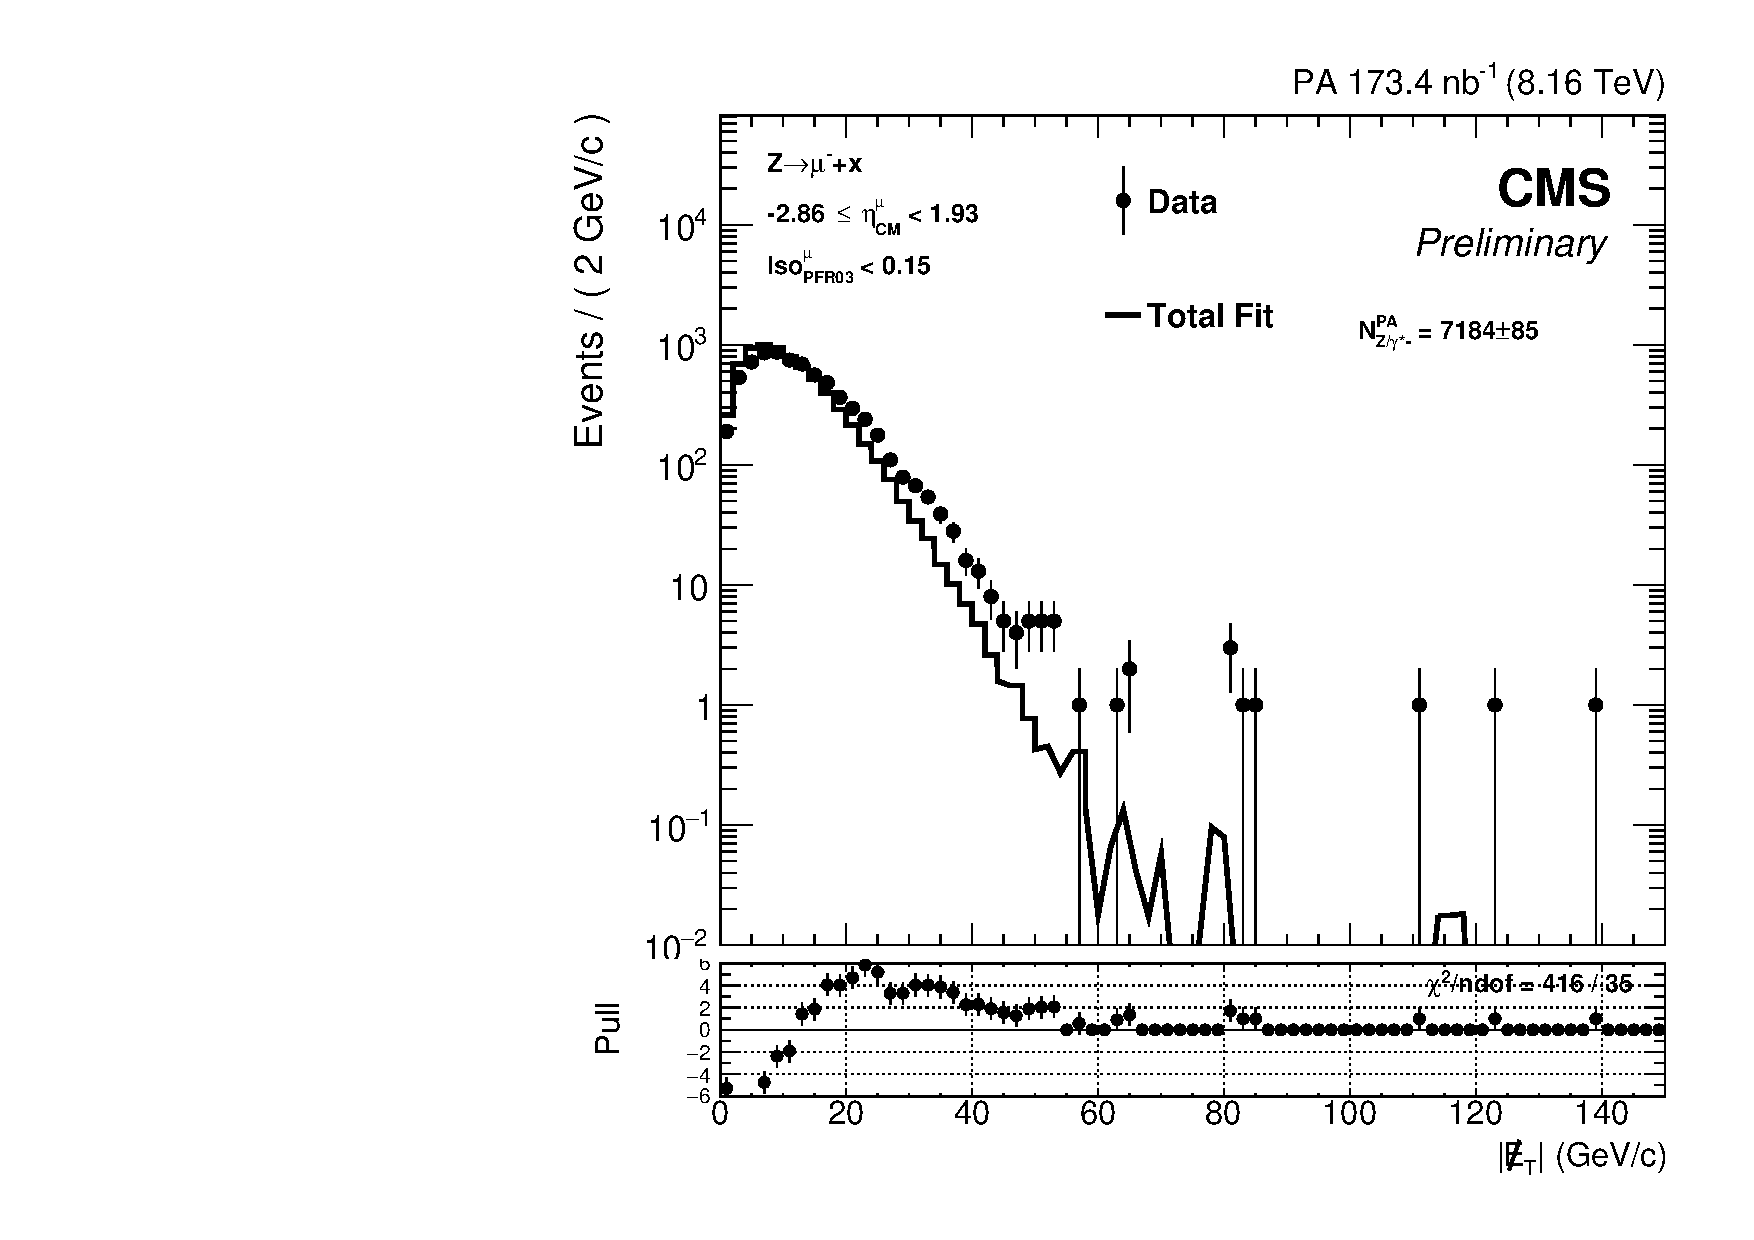
\includegraphics[width=0.4\textwidth]{Figures/WBoson/Analysis/Correction/Recoil/CheckFits/Z/METPF_RAW/PLOT_MET_DATA_ZToMuMi_PA_Model_TEMP_DY_MuEtaCM_m286_193_MuIso_0_15.pdf}
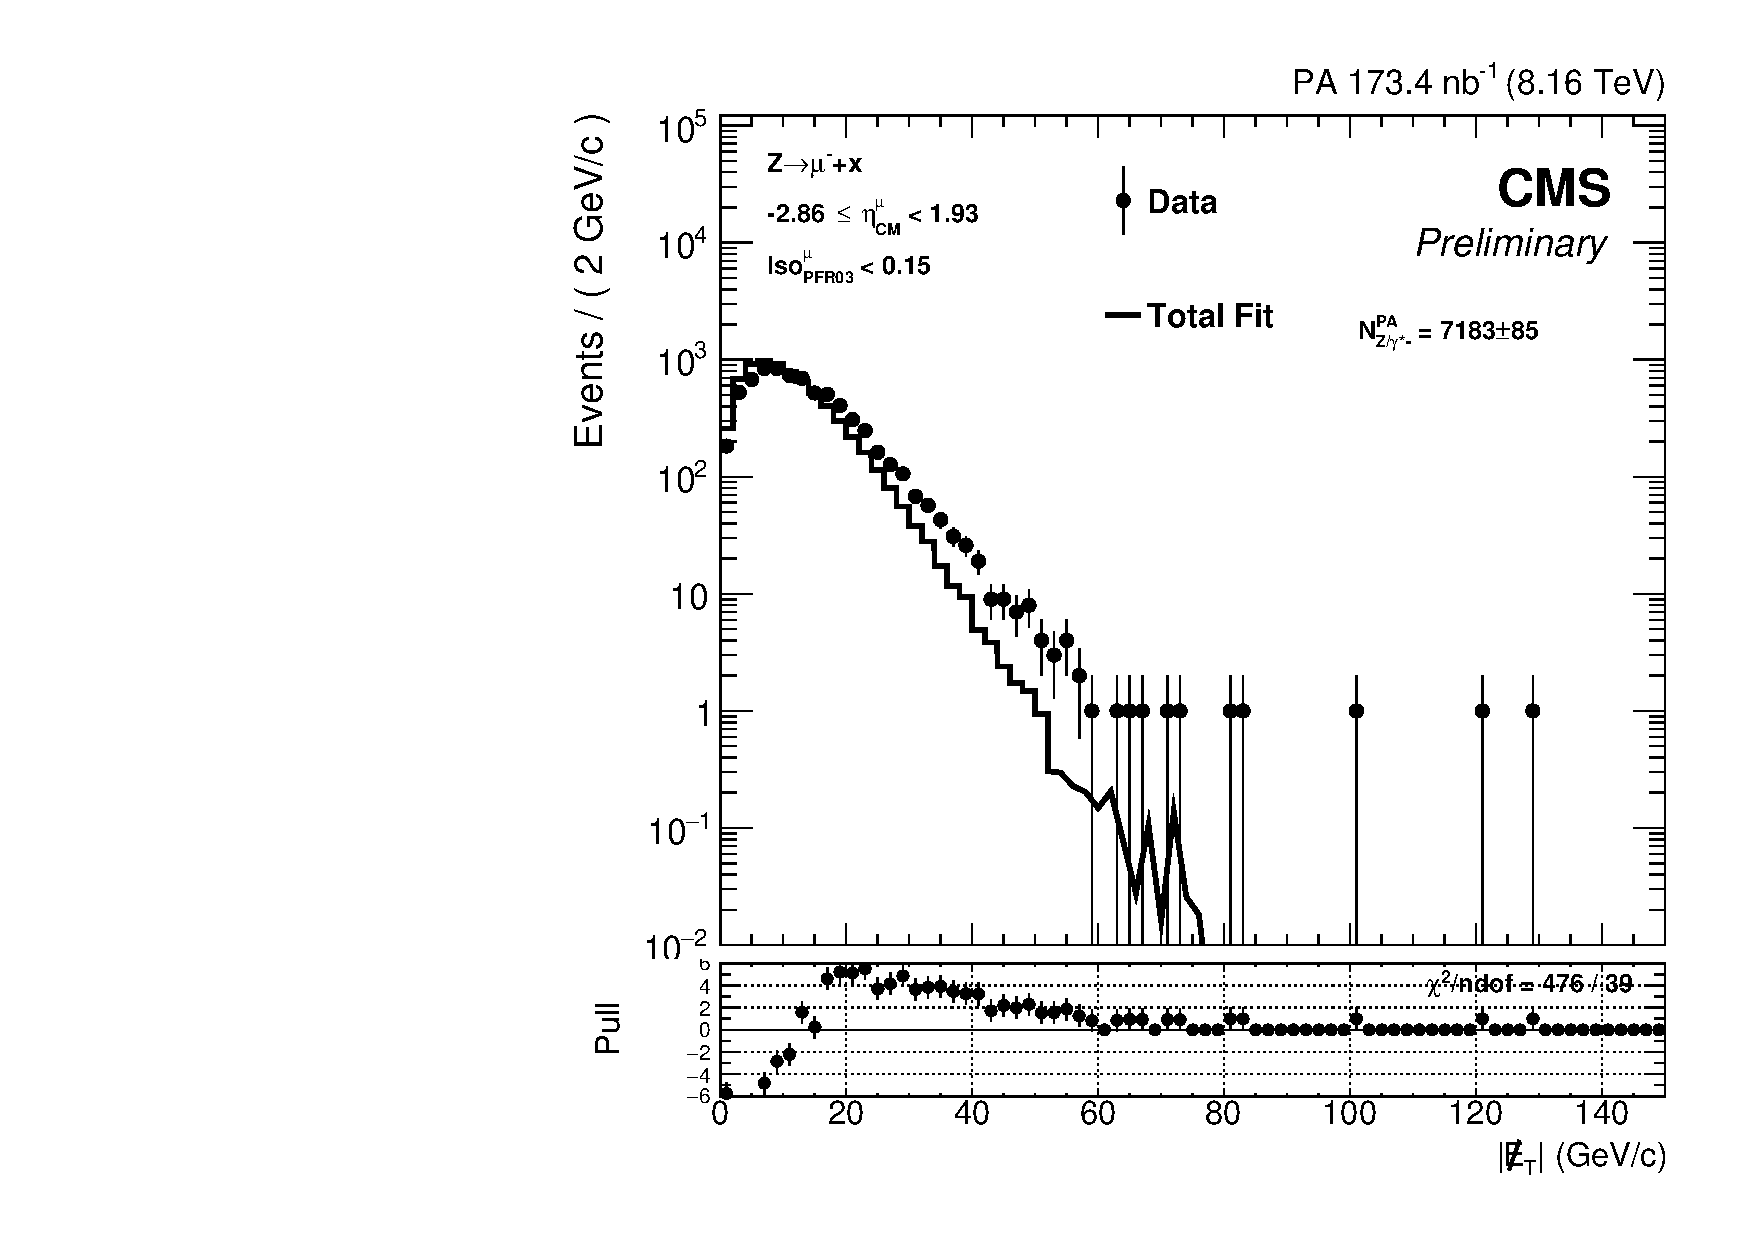
\includegraphics[width=0.4\textwidth]{Figures/WBoson/Analysis/Correction/Recoil/CheckFits/Z/METPF_Type1/PLOT_MET_DATA_ZToMuMi_PA_Model_TEMP_DY_MuEtaCM_m286_193_MuIso_0_15.pdf} \\
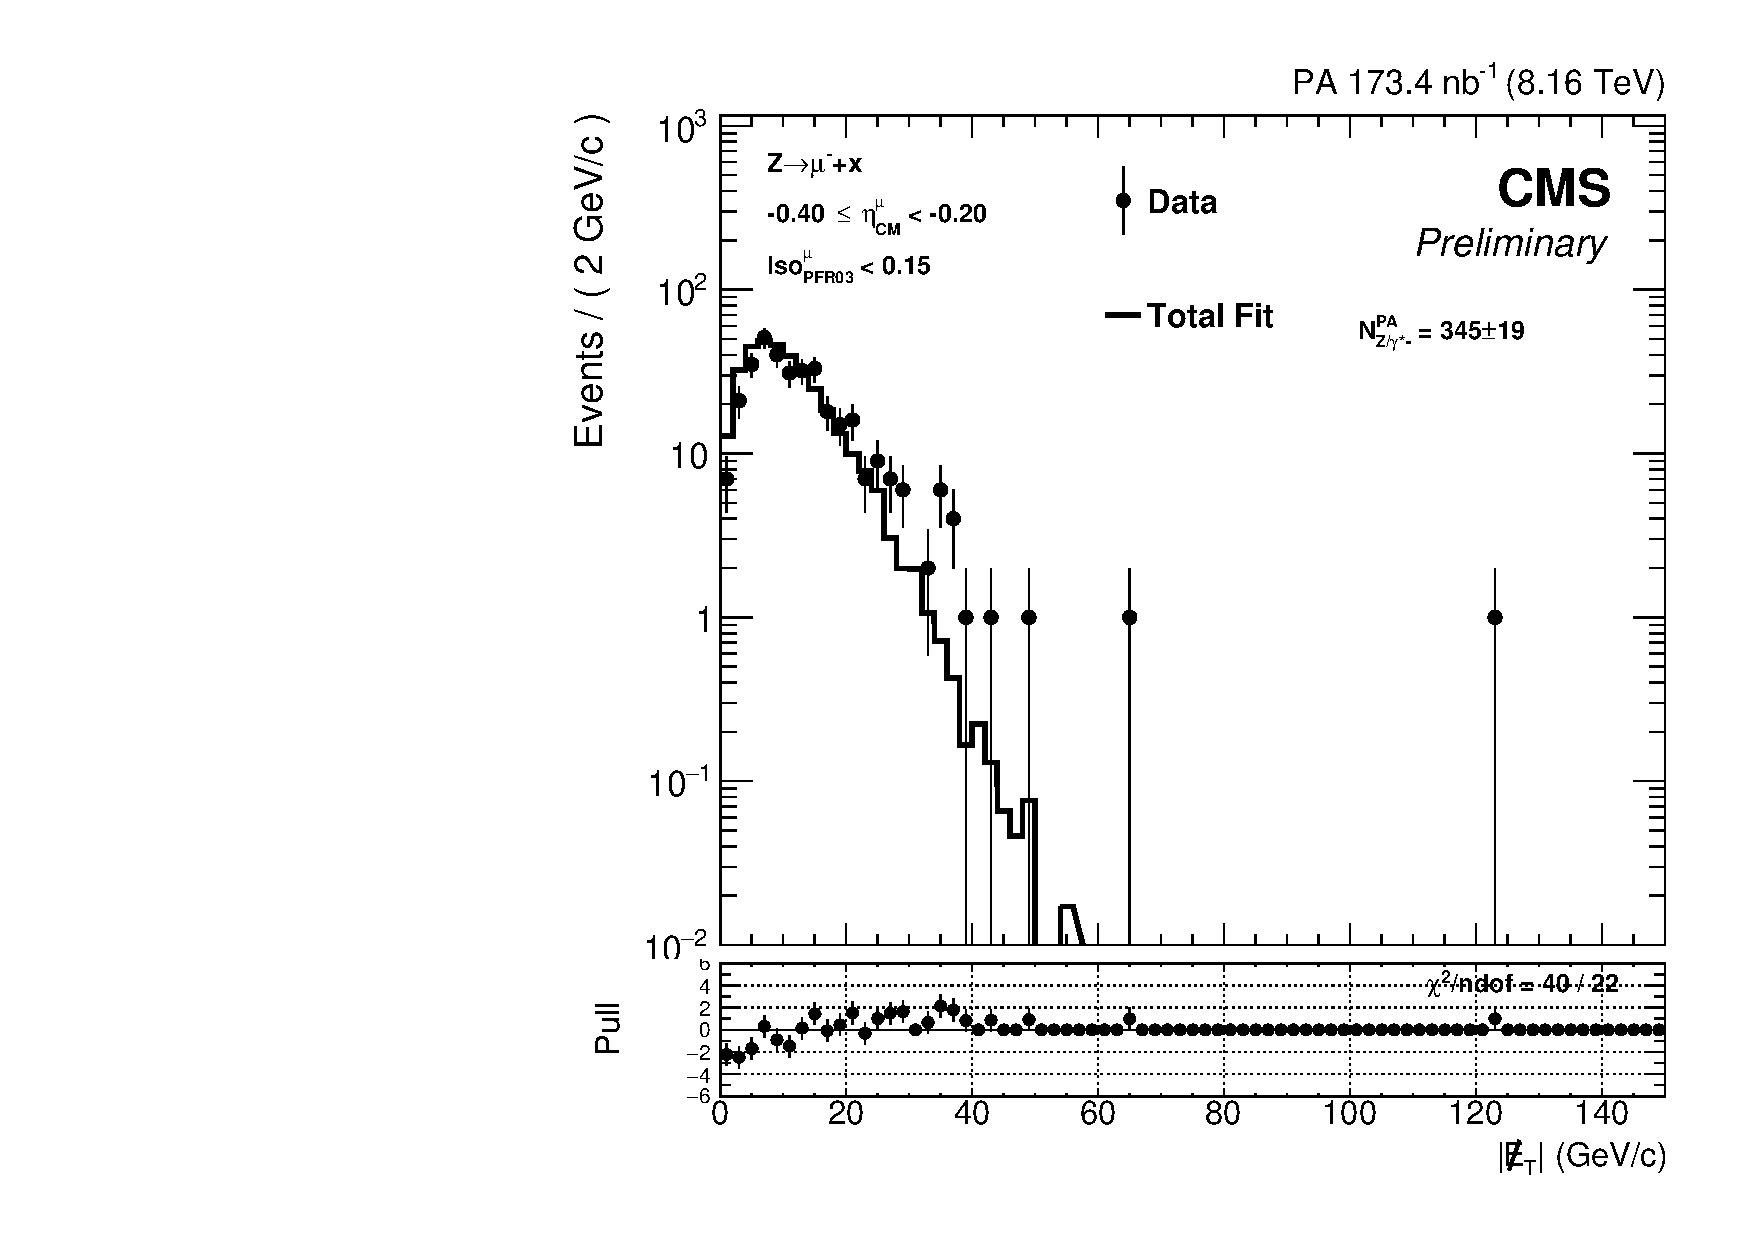
\includegraphics[width=0.4\textwidth]{Figures/WBoson/Analysis/Correction/Recoil/CheckFits/Z/METPF_RAW/PLOT_MET_DATA_ZToMuMi_PA_Model_TEMP_DY_MuEtaCM_m40_m20_MuIso_0_15.pdf}
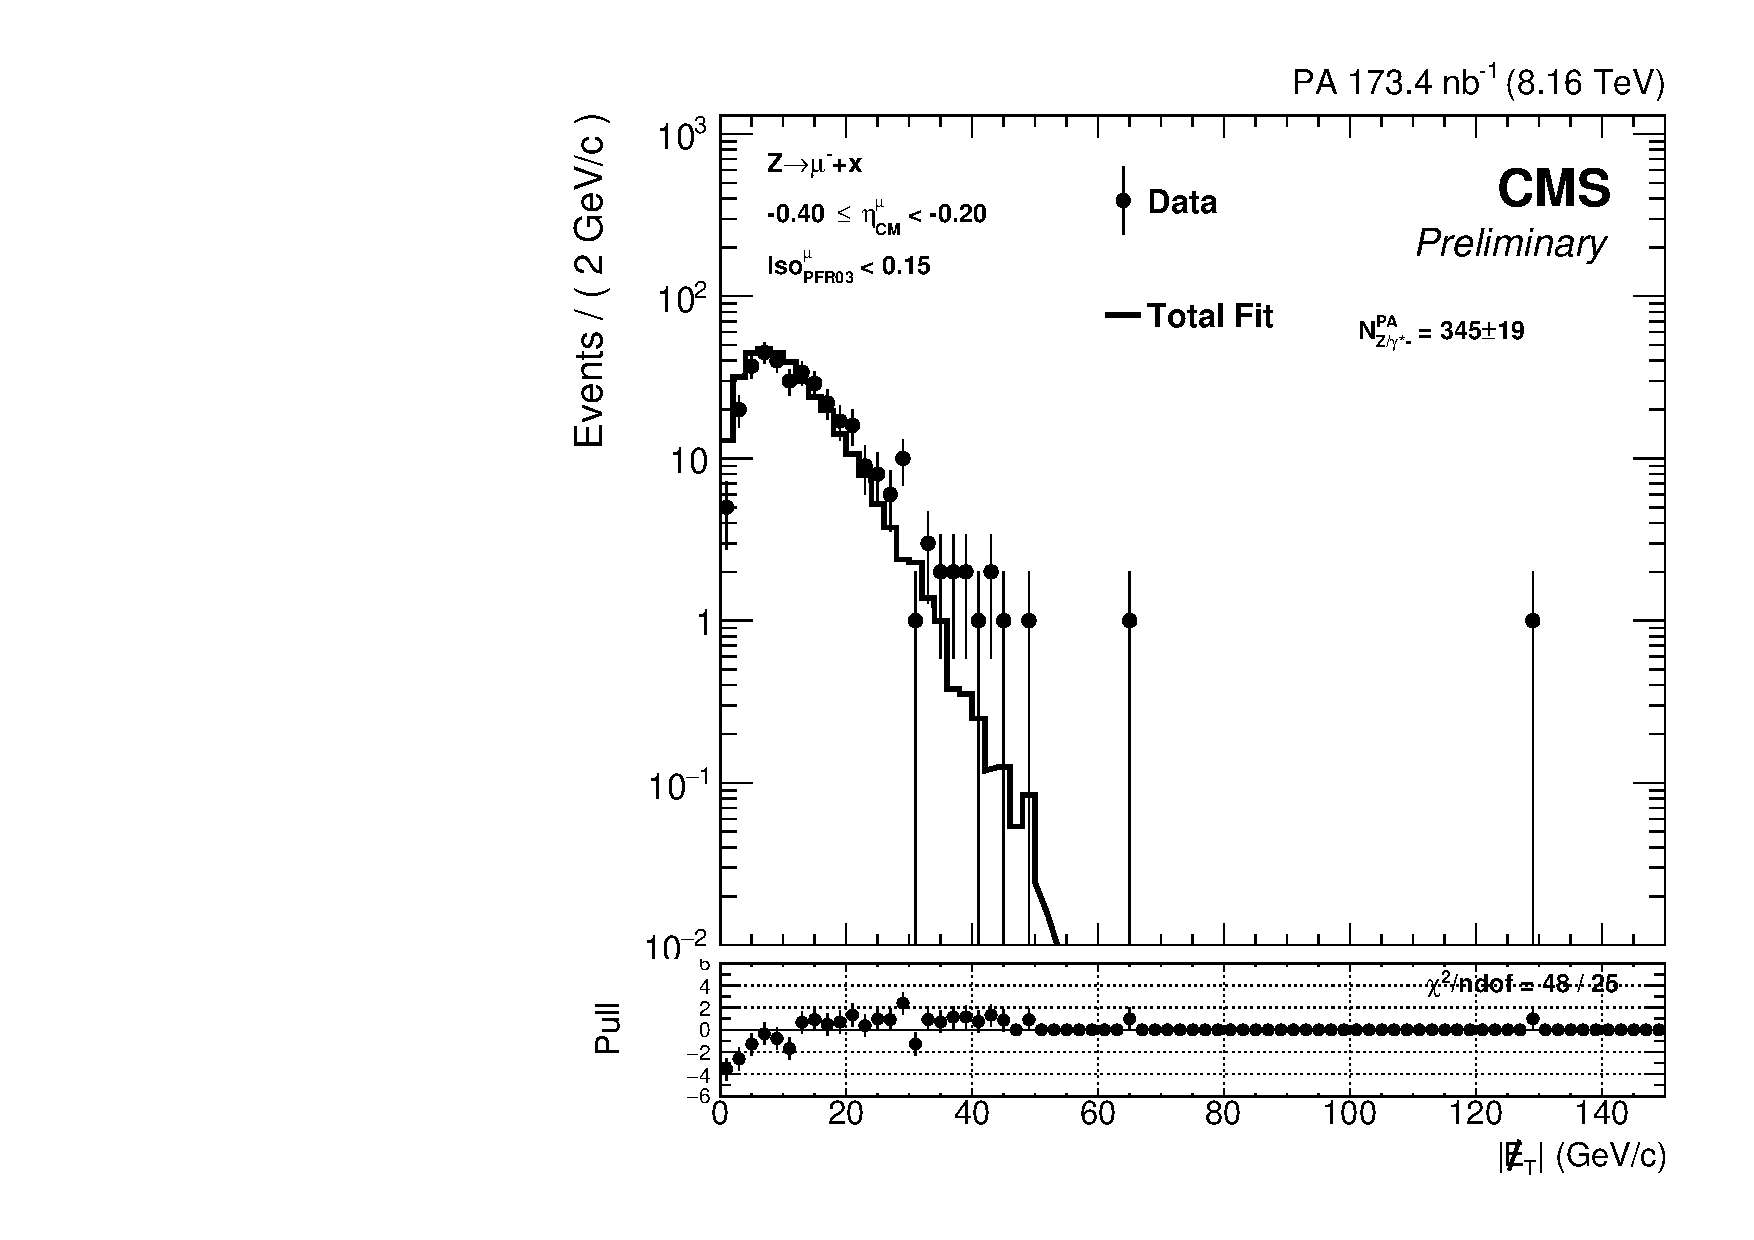
\includegraphics[width=0.4\textwidth]{Figures/WBoson/Analysis/Correction/Recoil/CheckFits/Z/METPF_Type1/PLOT_MET_DATA_ZToMuMi_PA_Model_TEMP_DY_MuEtaCM_m40_m20_MuIso_0_15.pdf}
\caption{A comparison of the MET distribution in data and MC for Z boson selected events. The top plots correspond to the full pseudorapidity range in the analysis while the bottom ones correspond to an specific pseudorapidity bin. The left plots use the PF MET RAW while the right ones the PF MET Type1.}
\label{fig:METtypeCheck}
\end{center}
\end{figure}

The event activity is not well modelled in the MC, though it is embedded in EPOS minimum bias events. This can have a significant impact on the the MET reconstruction (and also muon selection efficiency through the muon isolation, see \sect{sec:WBoson_Analysis_MuonIsolation}). In order to correct the effects of the mismodelling of the event activity in MC, a reweighting of the energy deposited in the Hadron Forward (HF) calorimeters (on both sides) is performed, as described in \sect{sec:WBoson_Analysis_EventActivityReweighting}. In \fig{fig:HFrewCheck} we show the comparison of the PF MET RAW distribution in data and MC for Z boson selected events, without (left) and with the HF energy reweighting (right). As we can observe, the low MET region in MC agrees better with the data distribution after applying the reweighting.

\begin{figure}[!h]
\begin{center}
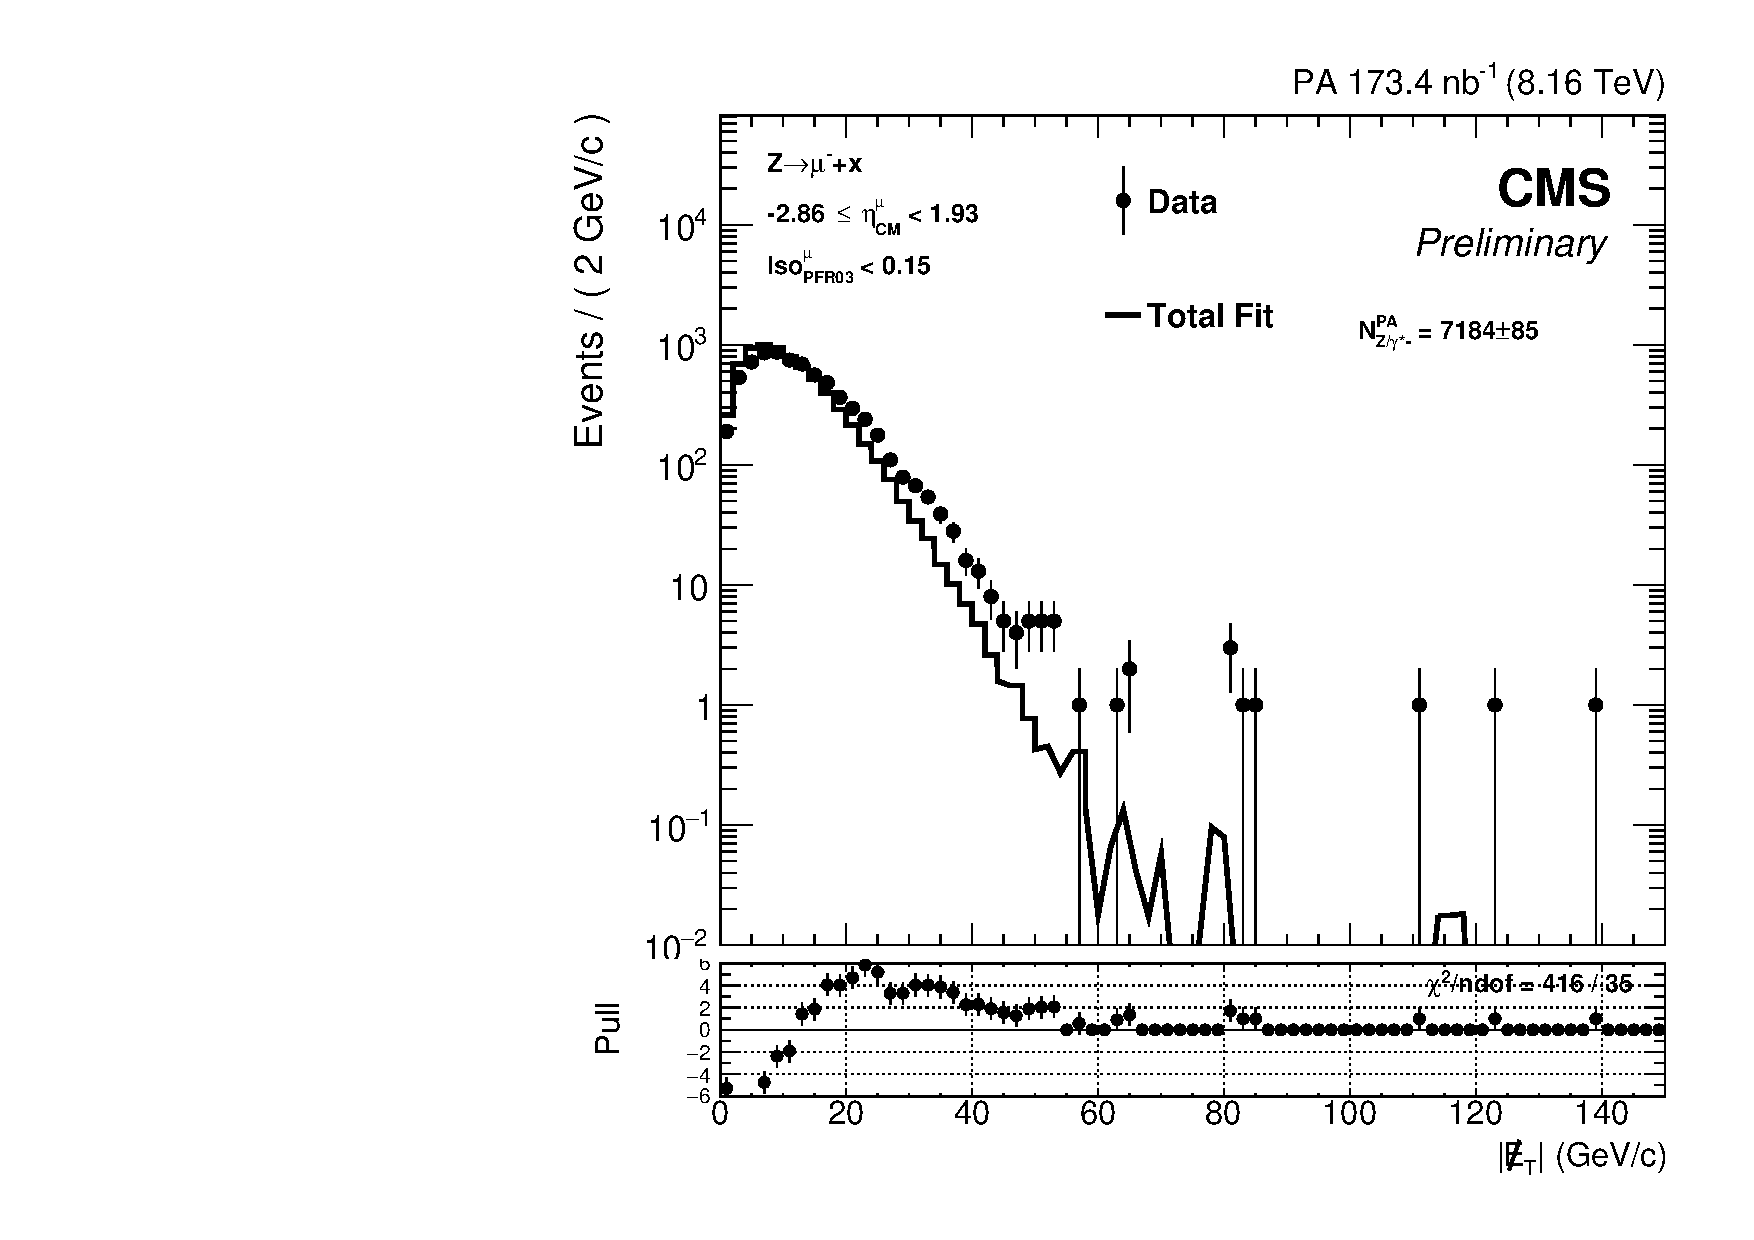
\includegraphics[width=0.4\textwidth]{Figures/WBoson/Analysis/Correction/Recoil/CheckFits/Z/METPF_RAW/PLOT_MET_DATA_ZToMuMi_PA_Model_TEMP_DY_MuEtaCM_m286_193_MuIso_0_15.pdf}
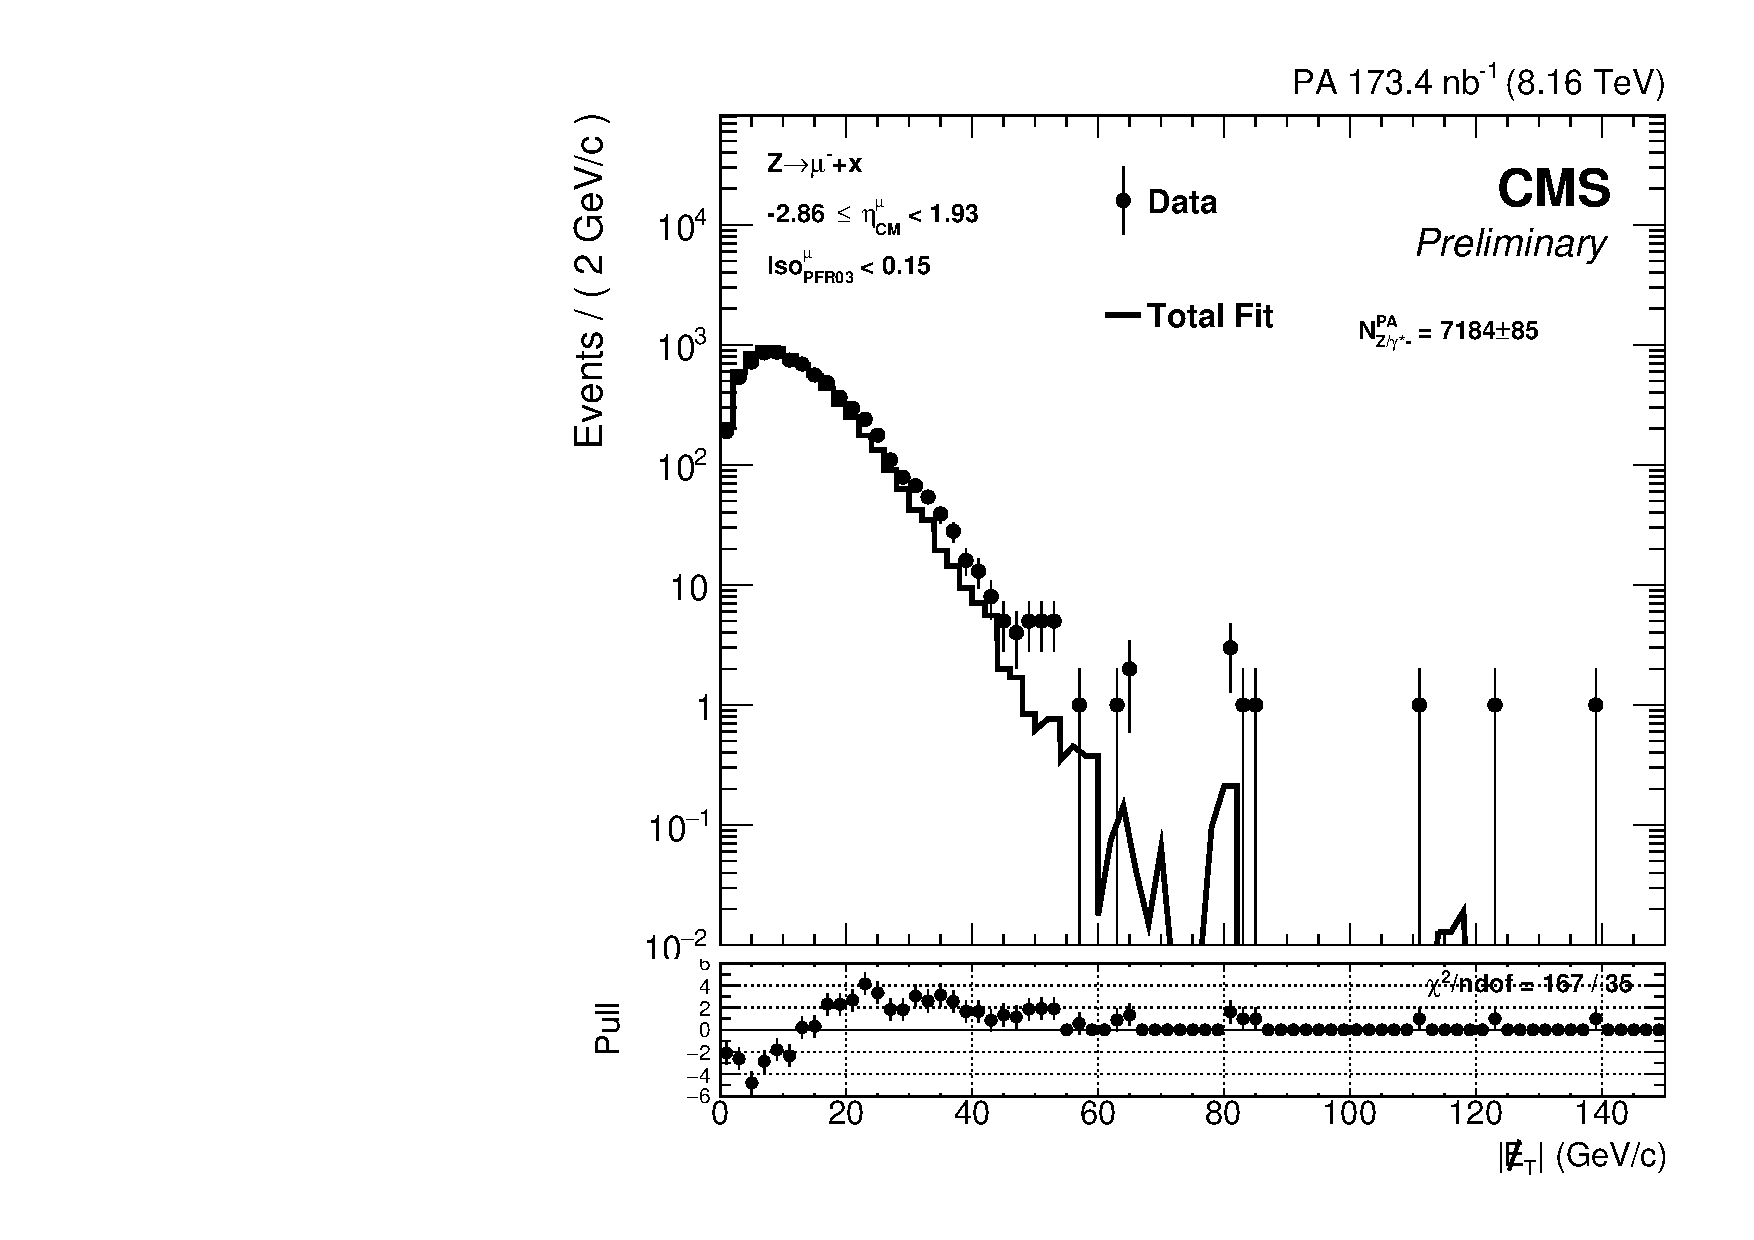
\includegraphics[width=0.4\textwidth]{Figures/WBoson/Analysis/Correction/Recoil/CheckFits/Z/METPF_RAW_HFrew/PLOT_MET_DATA_ZToMuMi_PA_Model_TEMP_DY_MuEtaCM_m286_193_MuIso_0_15.pdf} \\
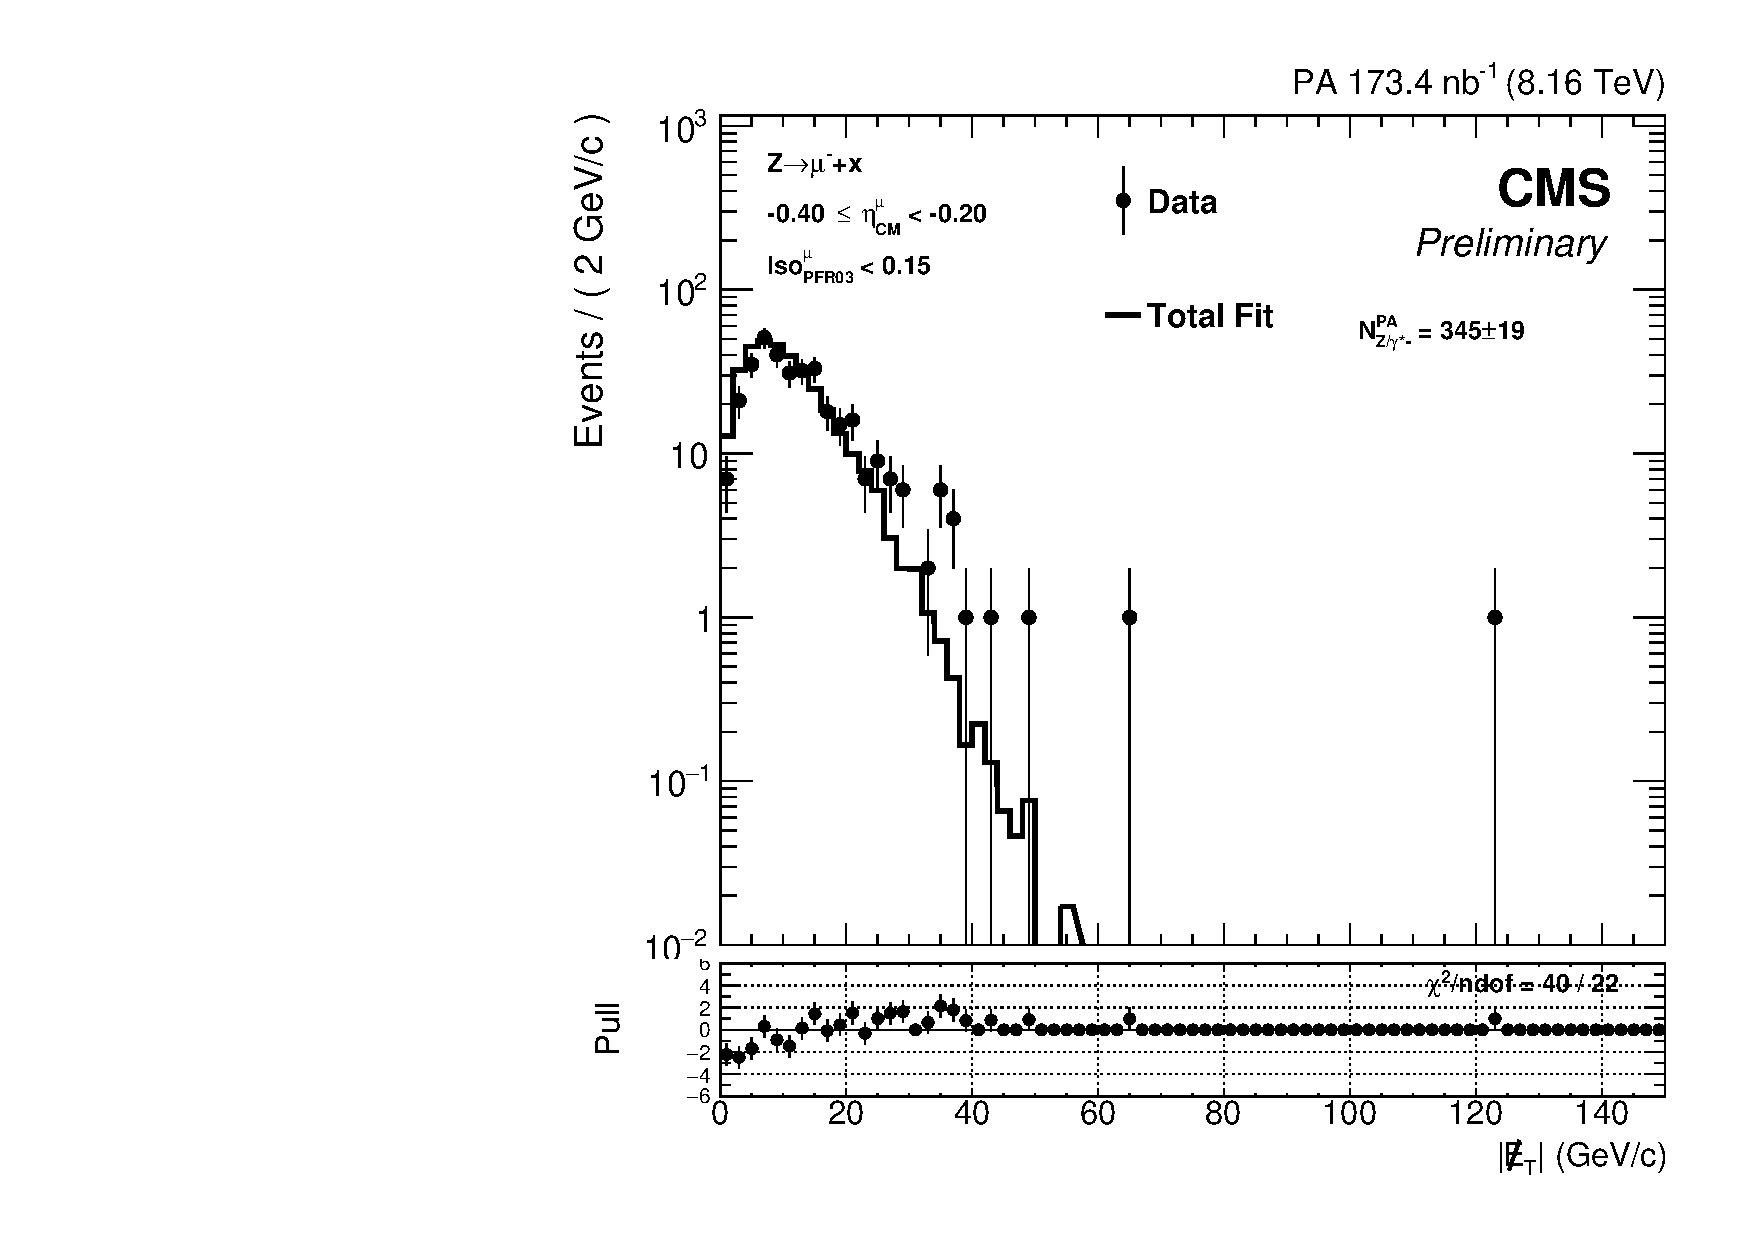
\includegraphics[width=0.4\textwidth]{Figures/WBoson/Analysis/Correction/Recoil/CheckFits/Z/METPF_RAW/PLOT_MET_DATA_ZToMuMi_PA_Model_TEMP_DY_MuEtaCM_m40_m20_MuIso_0_15.pdf}
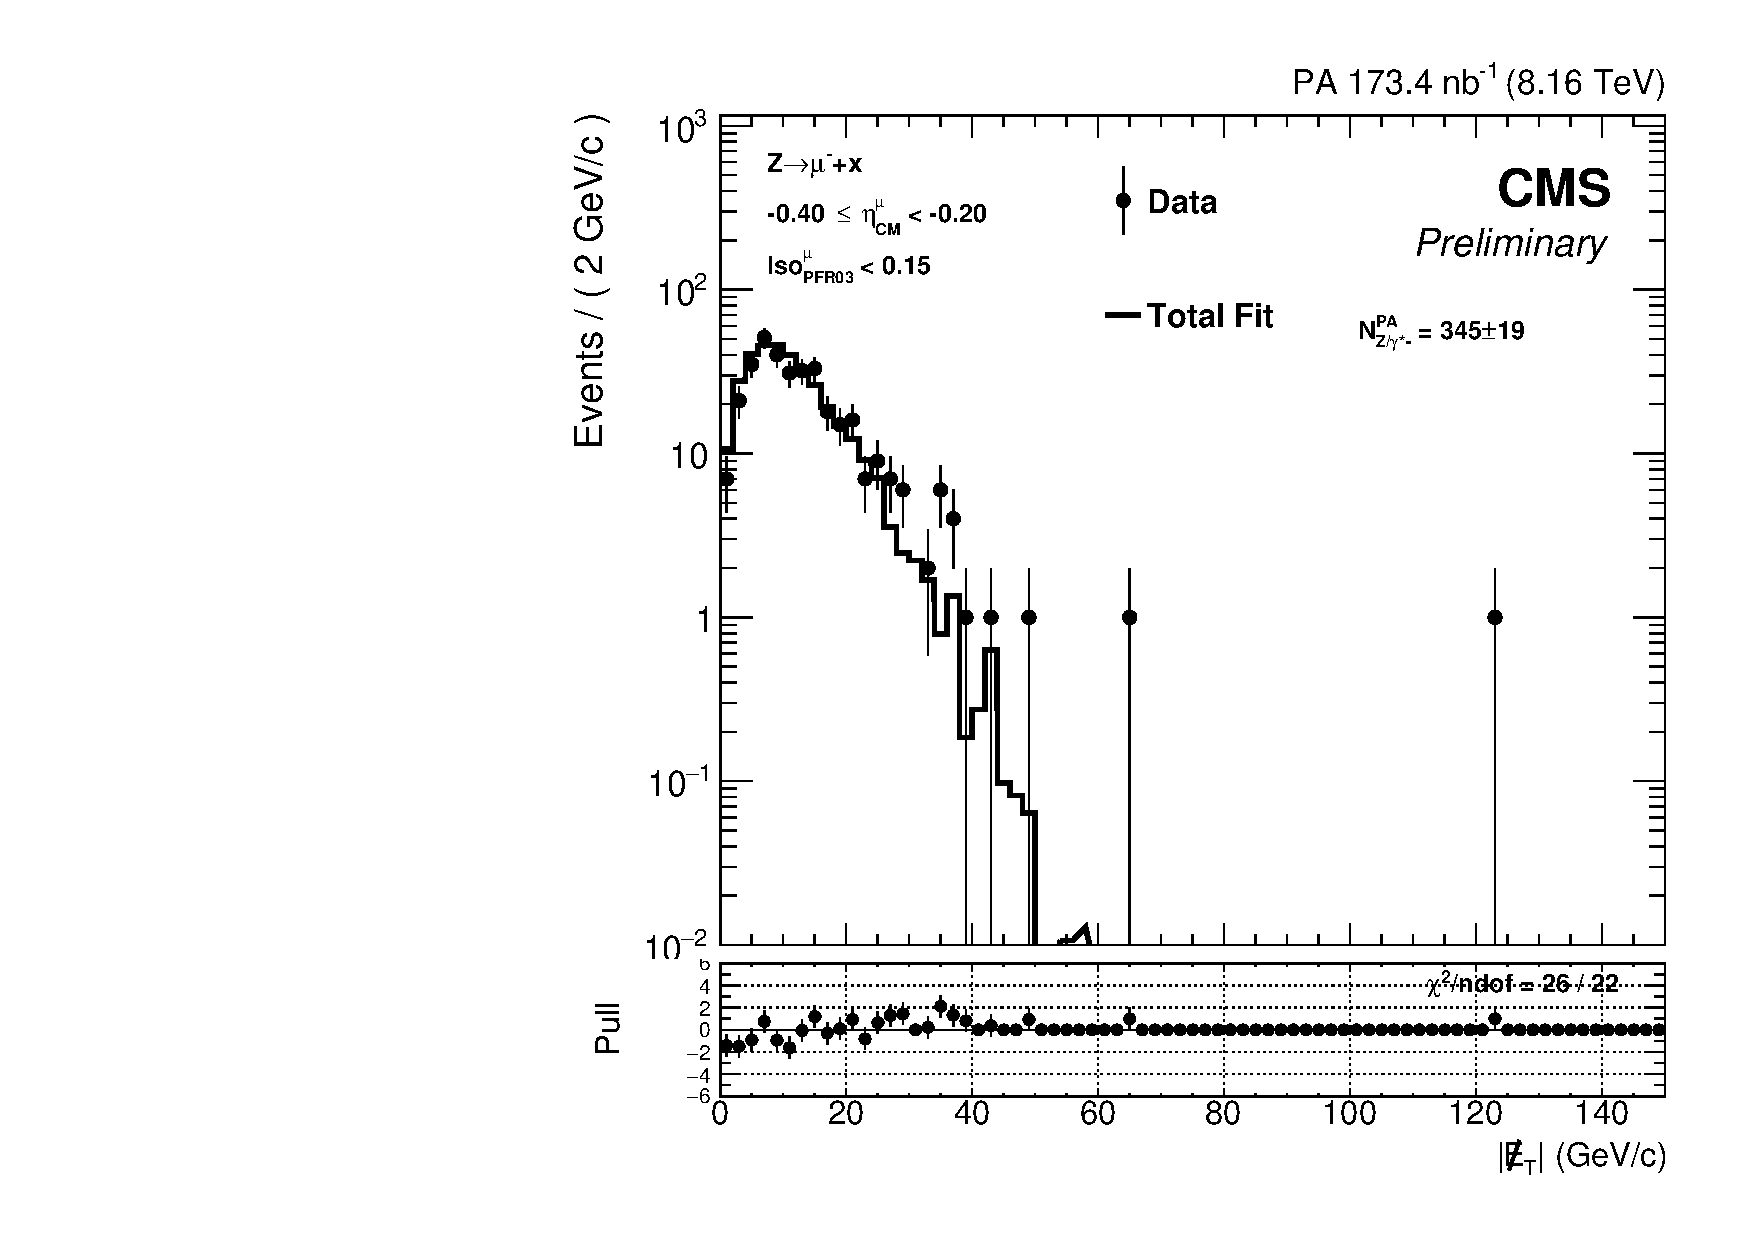
\includegraphics[width=0.4\textwidth]{Figures/WBoson/Analysis/Correction/Recoil/CheckFits/Z/METPF_RAW_HFrew/PLOT_MET_DATA_ZToMuMi_PA_Model_TEMP_DY_MuEtaCM_m40_m20_MuIso_0_15.pdf}
\caption{A comparison of the MET distribution in data and MC for Z boson selected events. 
The top plots correspond to the full pseudorapidity range in the analysis while the bottom ones correspond to an specific pseudorapidity bin. The left plots use the PF MET RAW without HF reweighting in MC, while the right ones the MC events are reweighed.}
\label{fig:HFrewCheck}
\end{center}
\end{figure}

In addition, in Appendix \ref{app:met_nohf_check} the impact of the HF detector on the MET determination has been further checked. The agreement between MC and data METs is compared using the PF MET RAW with HF reweighting for MC, with the one obtained with the MET distributions measured excluding the HF contribution. It has been observed that the agreement between MC and data MET is better using PF MET RAW with HF reweighting for MC. After the studies performed above we conclude that the best MET to use in the analysis is the PF MET RAW with HF reweighting for MC. 

Finally, a correction, derived using the hadronic recoil technique \cite{MET_Recoil}, has to be applied to correct the recoil scale and resolution in MC to better match those in data. This correction improves the matching between the MET distributions in data and MC. The correction procedure is described in the following subsections.


\subsubsection{Definition of recoil} \label{sec:WBoson_Analysis_RecoilCorrection}

The recoil of \ZToMuMu events is defined as the vector sum of the transverse momenta of all particle flow candidates excluding the muons from the boson decay. Since the MET is defined as the negative of the vector sum of all particle flow candidates in the events, one can express the recoil vector as:

\begin{equation}\label{eq:equT} 
\vec{u_{T}} = -\vec{E\!\!\!/{_T}} - \vec{q}_{T},
\end{equation}

where $\vec{u_{T}}$ is the hadronic recoil in the transverse plane to the beam direction and $\vec{q_{T}}$ is the transverse momentum of the dimuon system. For the \WToMuNu events, the recoil is defined as:

\begin{equation}\label{eq:equTW}
\vec{u_{T}} = -\vec{E\!\!\!/{_T}} - \vec{p}_{T}^{\mu},
\end{equation}

where $\vec{p}_{T}^{\mu}$ is the transverse momentum of the muon.

The recoil vector is projected along the transverse plane in the boson direction, and the parallel and perpendicular components of the recoil vector with respect to the boson transverse momentum are labelled as $u_{\parallel}$ and $u_{\perp}$, respectively. \fig{fig:RecoilDefinition} describes the recoil and its components.

\begin{figure}
\begin{center}
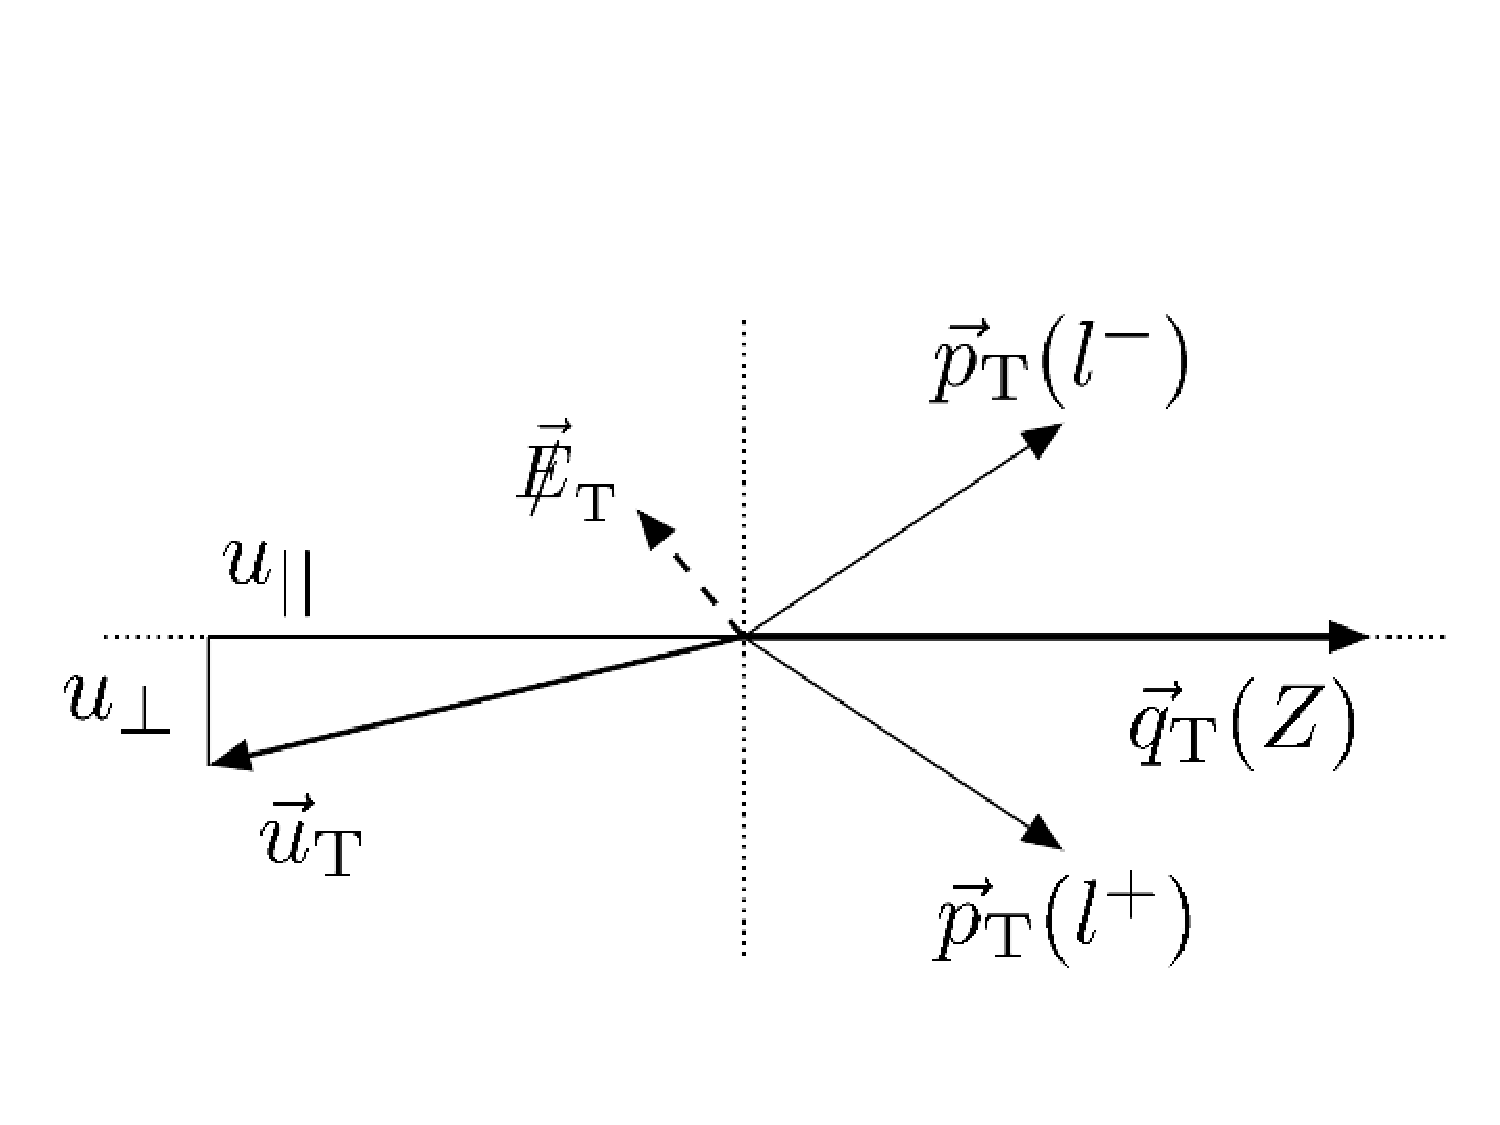
\includegraphics[width=0.4\textwidth]{Figures/WBoson/Analysis/Correction/Recoil/Recoil_Definition.pdf}
\caption{Definition of the recoil vector and its components for \ZToMuMu events.}
\label{fig:RecoilDefinition}
\end{center}
\end{figure}
 
In the determination of the boson transverse momentum vector $\vec{q}_{T}$, the reconstructed muon information is used whenever possible. The following criteria are used to determine the $q_{T}$ depending on the MC sample:

\begin{itemize}

\item \WToMuNu MC: The boson momentum is derived from the sum of the reconstructed leading muon \pt and the generated neutrino \pt.
\item \WToTauNu MC: The boson momentum is taken from the generated \W boson \pt.
\item \ttbar MC: The boson momentum is taken from the generated \W boson \pt.
\item \DYToTauTau MC: The boson momentum is taken from the generated \DY boson \pt.
\item \DYToMuMu MC (DY control region): The boson momentum is determined from the sum of the two reconstructed muons.
\item \DYToMuMu MC (\W signal region): In the case of Drell-Yan events that enter as background in the \W boson signal region (i.e. events which are not rejected by the Drell-Yan veto), these events are divided in two categories based on the sub-leading muon:
\begin{itemize}
\item If the sub-leading muon was not reconstructed (falls outside of the coverage of the CMS detector), the sub-leading muon is treated in the same way as a neutrino, the boson momentum is defined as the sum of the reconstructed leading muon \pt and the generated sub-leading muon \pt.
\item If the sub-leading muon was reconstructed, but it was not identified as a good quality muon because it fails one or more of the selection criteria, then the case is treated similar to the Drell-Yan control sample by defining the boson momentum as the sum of the reconstructed leading and sub-leading muon momenta.
\end{itemize}
\end{itemize}

In order to exclude muons from the underlying event distribution embedded in the signal MC samples, only reconstructed muons matched to a generated muon coming from the Electro-Weak decay process corresponding to the MC sample are considered.

The recoil corrections are extracted from the Z control sample. In order to determine them, the parallel and perpendicular components of the recoil vector are determined event by event in data and MC, and their distributions are sorted in bins of $q_{T}$. These distributions are fitted with an unbinned maximum likelihood fit using a weighted sum of two Gaussian functions:

\begin{equation}\label{eq:gaussFit}
n(u_{\parallel(\perp)}) = N \cdot \left( f \cdot  e^{\frac{(u_{\parallel(\perp)} - \mu_{1})^{2}}{2 \cdot \sigma_{1}^{2}}}  + (1-f)\cdot e^{\frac{(u_{\parallel(\perp)} - \mu_{2})^{2}}{2 \cdot \sigma_{2}^{2}}}  \right) \quad,
\end{equation}

where N corresponds to the number of events in each  $q_{T}$ bin, $f$ is the weight of the Gaussian components, $\mu_{1(2)}$ is the mean of each Gaussian, and  $\sigma_{1(2)}$ the corresponding width. A combination of two Gaussian functions was chosen to better describe the shape of the recoil distributions, both in data and MC. The following parameters where fixed/constrained to obtain a better convergence, after prior fitting attempts with all the parameters free: 

\begin{itemize}
\item $f = 0.70$ in data fits and $f = 0.45$ in MC fits, both for the parallel and perpendicular recoil components
\item $\mu_{2} = \mu_{1}$, except for the parallel component of the recoil in the MC fits
\end{itemize}

Examples of the distributions of the parallel and perpendicular recoil components, denoted as $u_{1}$ and $u_{2}$ respectively, are shown in \fig{fig:RecoilFitsData} for data and \fig{fig:RecoilFitsMC} for MC. Also the fits performed for the weighted combination of Gaussian functions as in \eq{eq:gaussFit}, and the pull distributions are shown.

\begin{figure}
\begin{center}
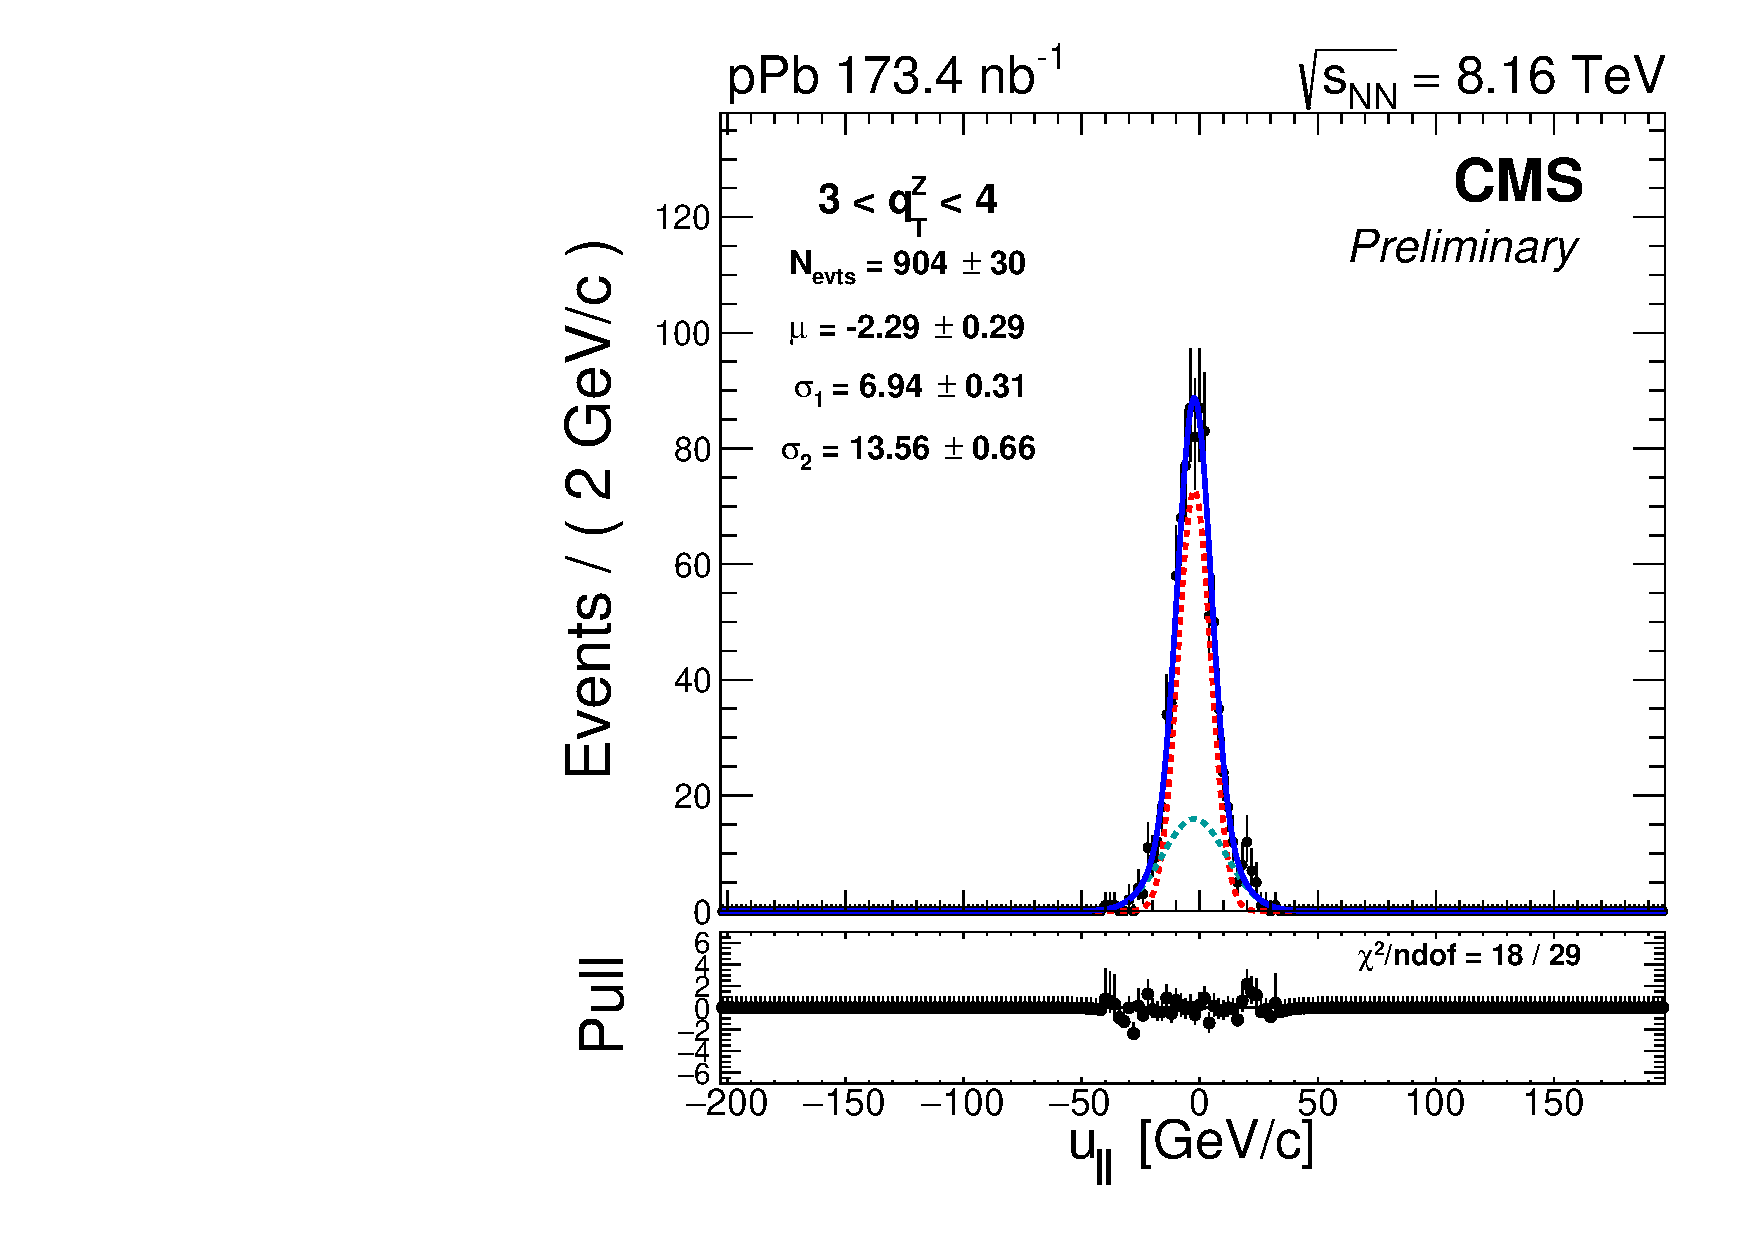
\includegraphics[width=0.4\textwidth]{Figures/WBoson/Analysis/Correction/Recoil/RecoilFits/Data/pfu1fit_2.pdf}
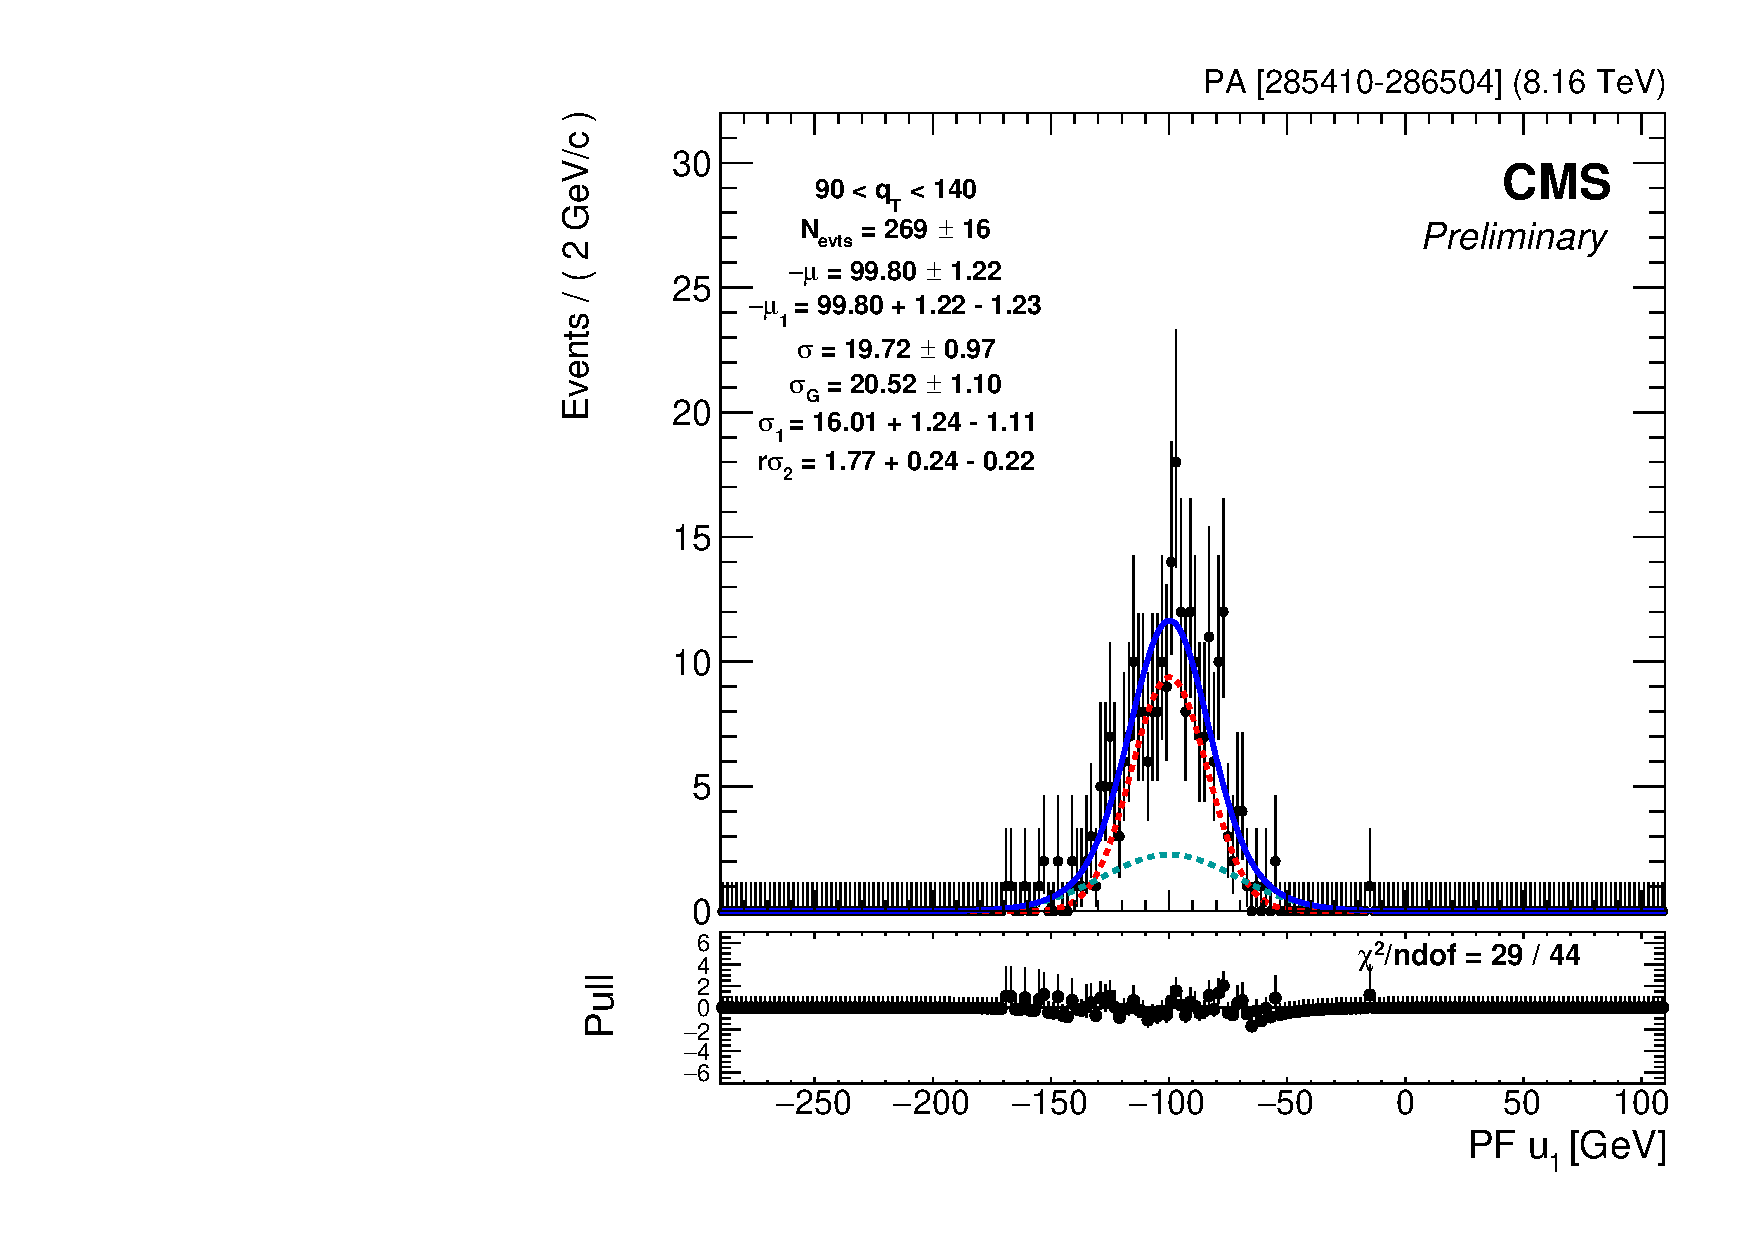
\includegraphics[width=0.4\textwidth]{Figures/WBoson/Analysis/Correction/Recoil/RecoilFits/Data/pfu1fit_29.pdf} \\
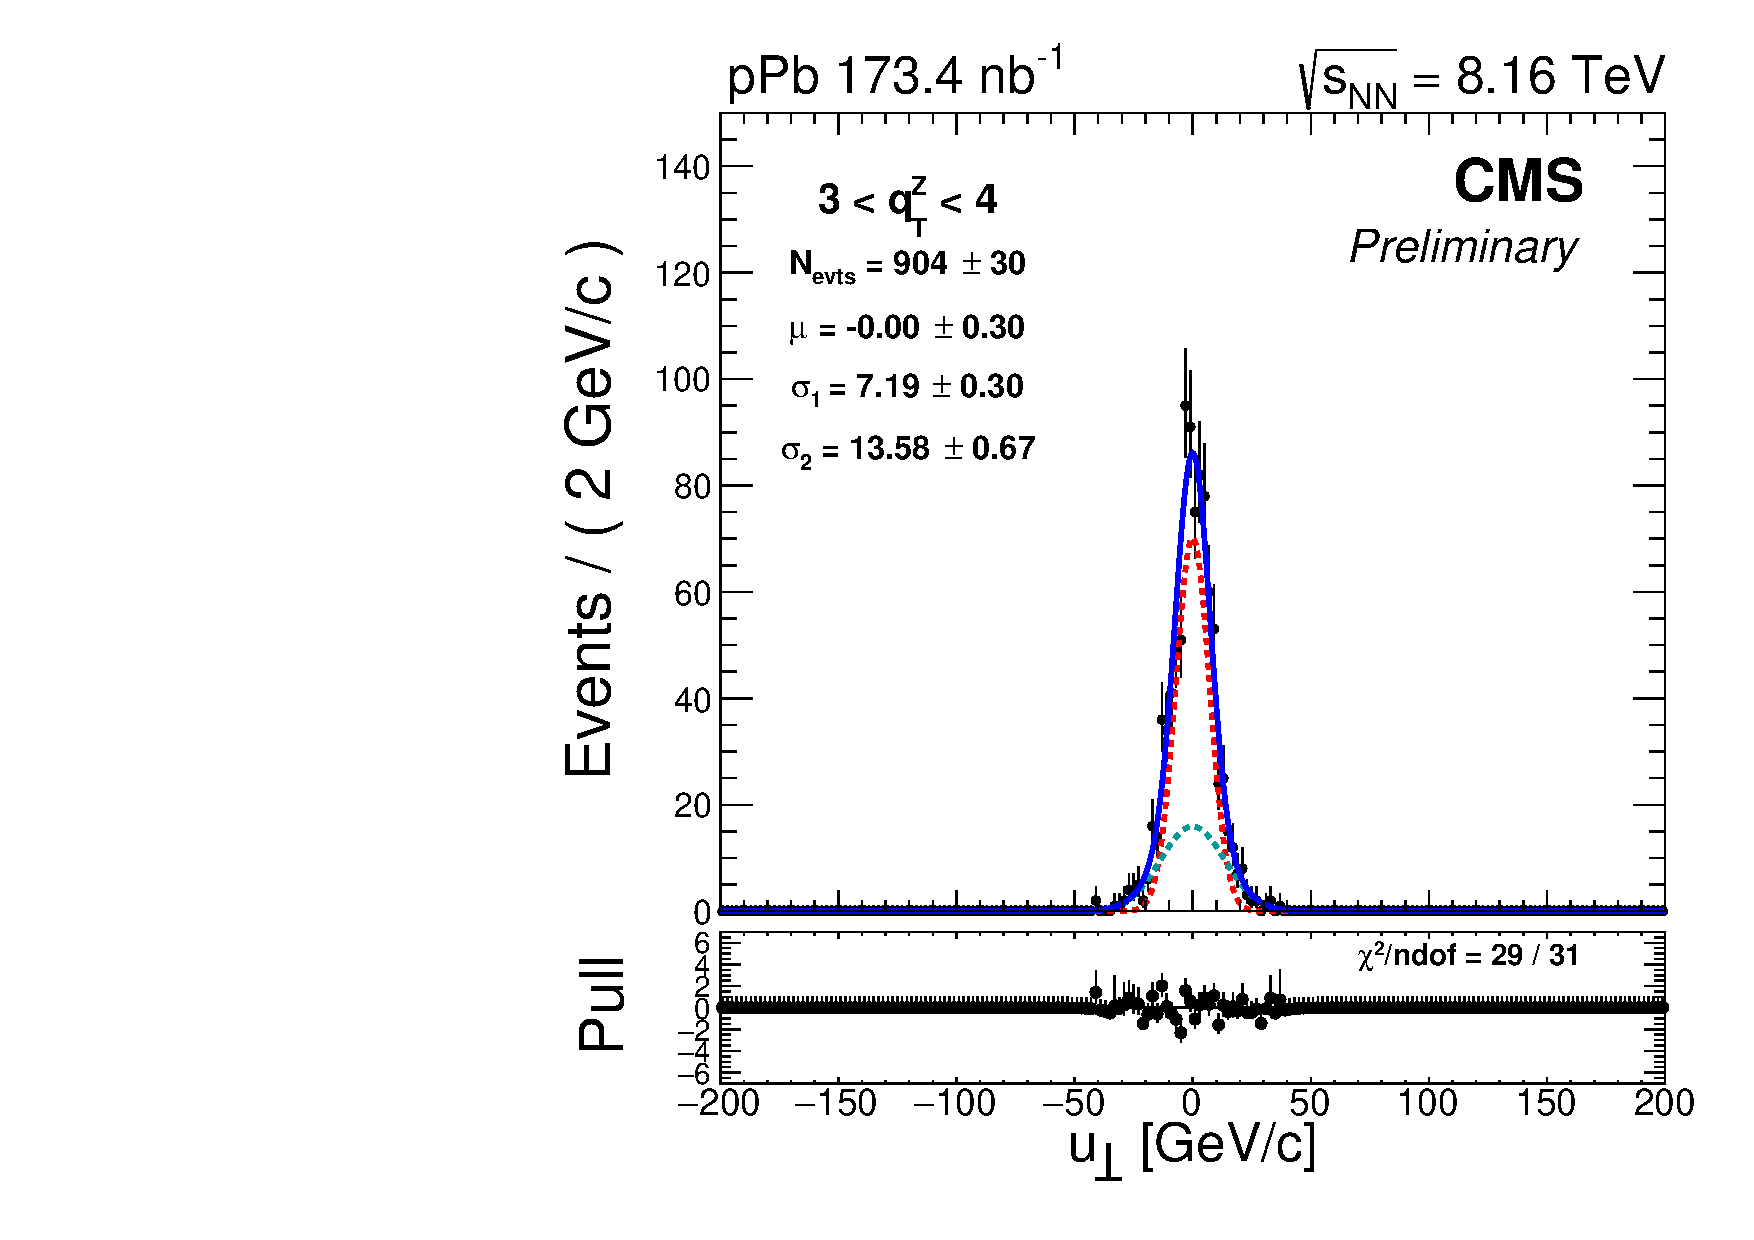
\includegraphics[width=0.4\textwidth]{Figures/WBoson/Analysis/Correction/Recoil/RecoilFits/Data/pfu2fit_2.pdf}
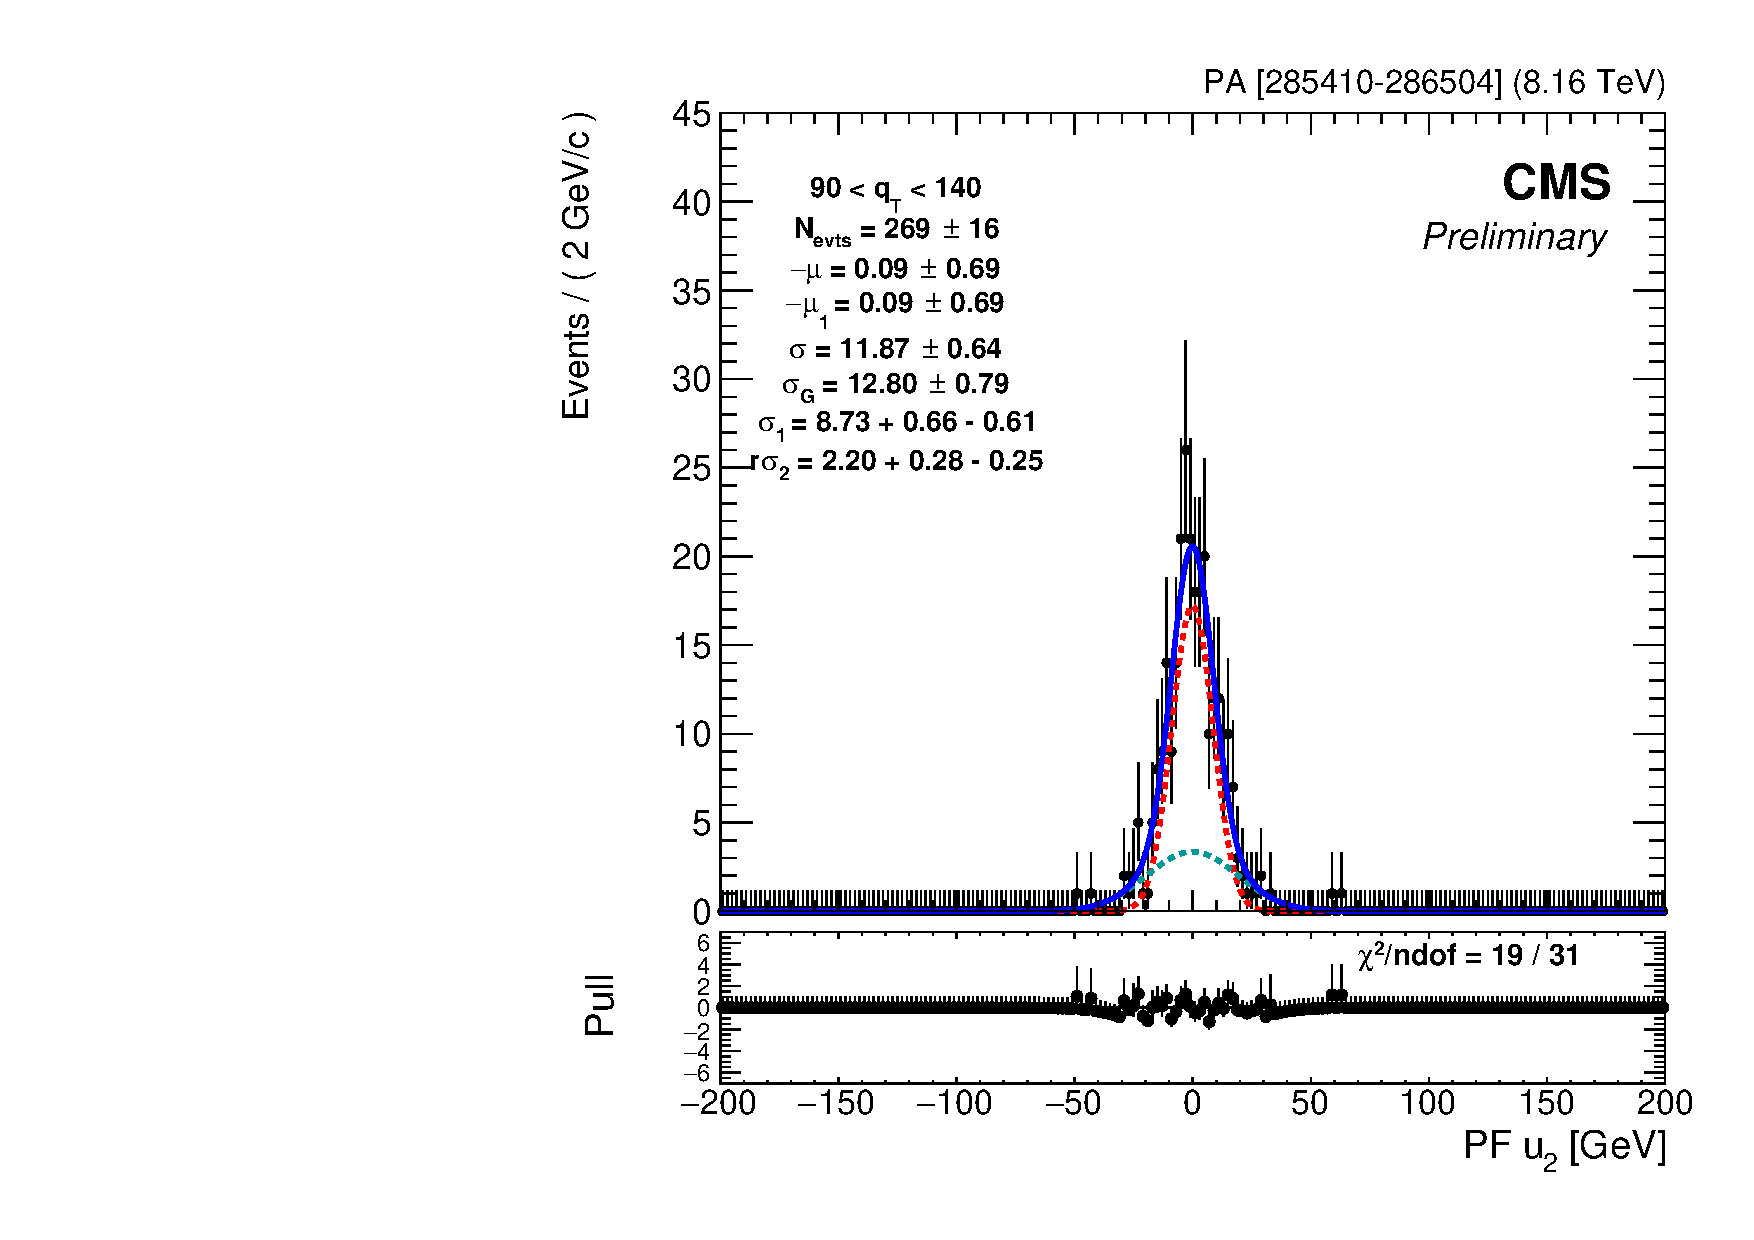
\includegraphics[width=0.4\textwidth]{Figures/WBoson/Analysis/Correction/Recoil/RecoilFits/Data/pfu2fit_29.pdf}
\caption{Distributions of the parallel (top) and perpendicular (bottom) components of the recoil in data with the fits performed with the weighted sum of two Gaussian functions in \eq{eq:gaussFit}. The distributions are for the $q_{T}$
bins 3 GeV $< q_{T} <$ 4 GeV (left) and 90 GeV $< q_{T} <$ 140 GeV (right).}
\label{fig:RecoilFitsData}
\end{center}
\end{figure}

\begin{figure}
\begin{center}
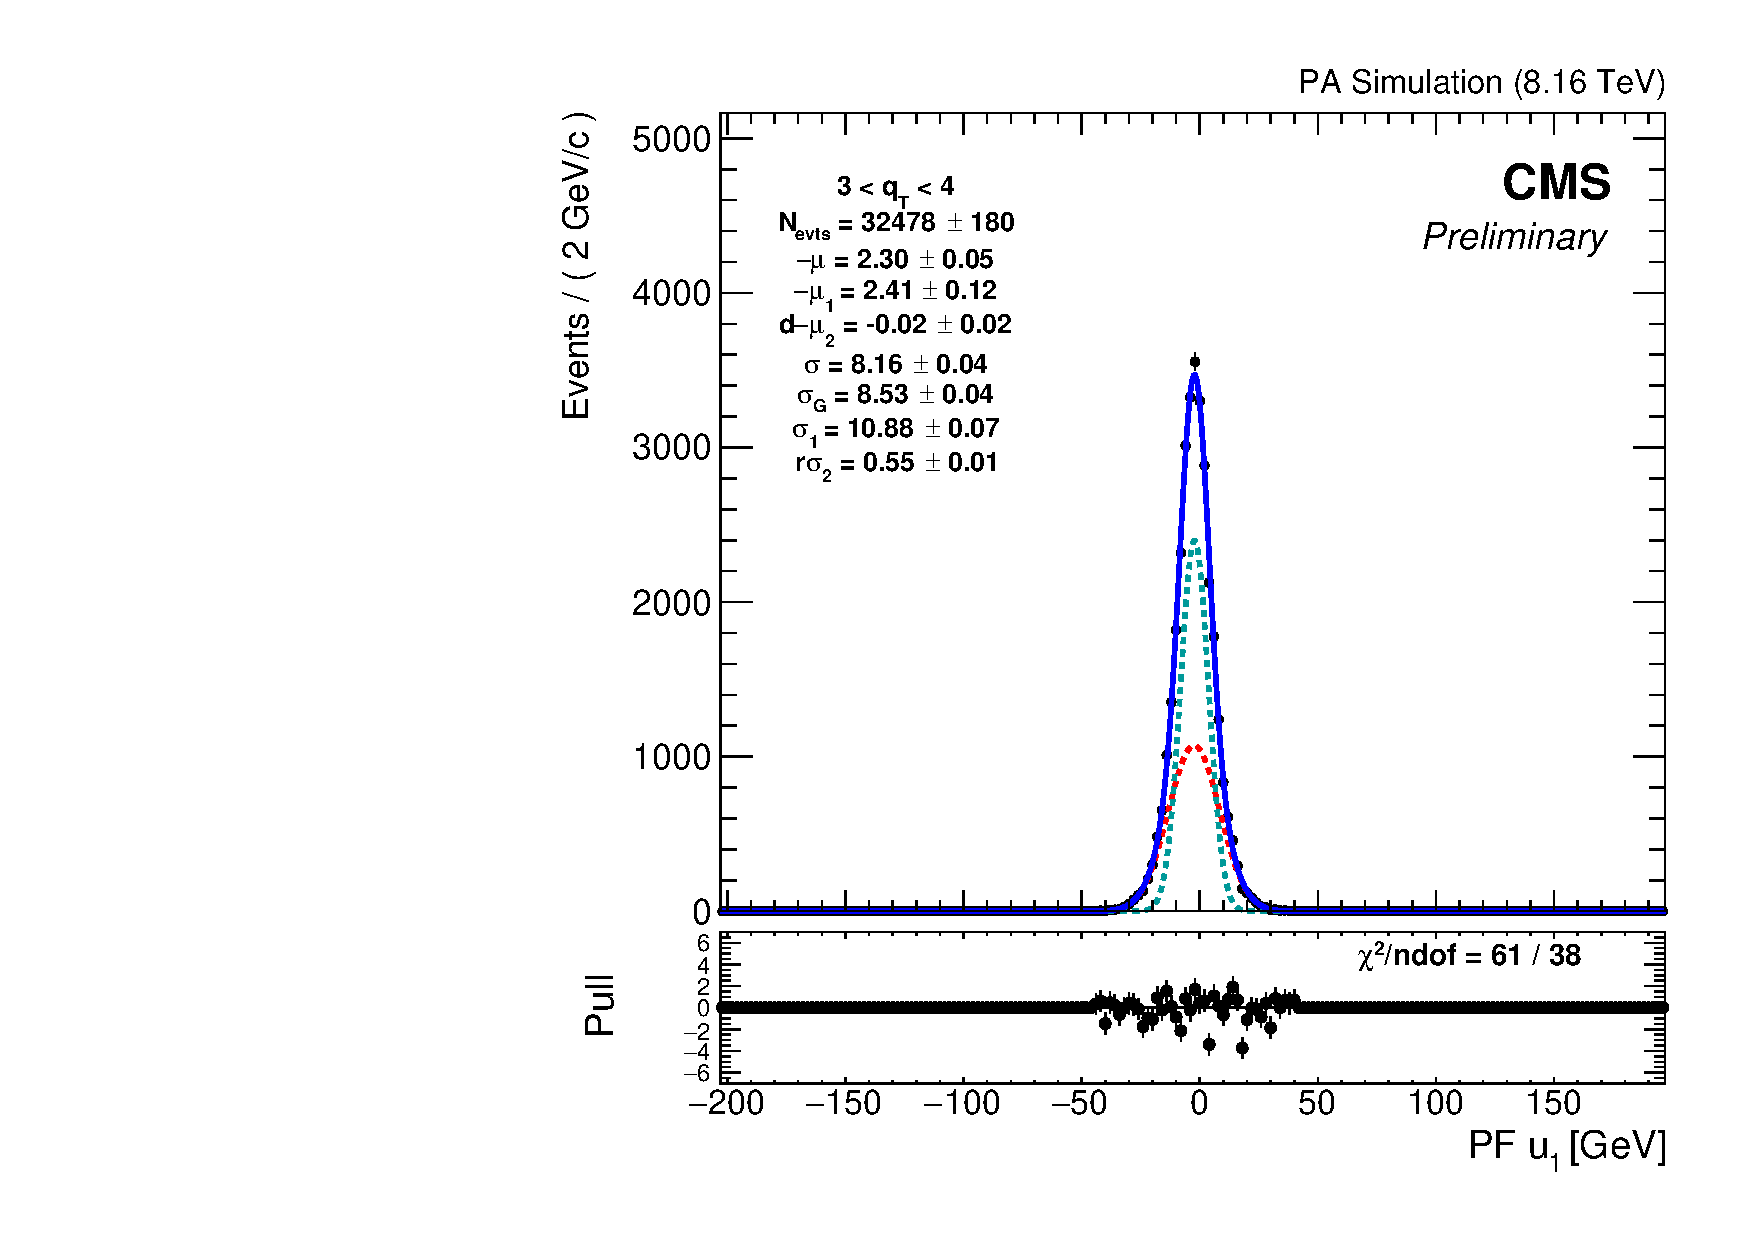
\includegraphics[width=0.4\textwidth]{Figures/WBoson/Analysis/Correction/Recoil/RecoilFits/MC/pfu1fit_2.pdf}
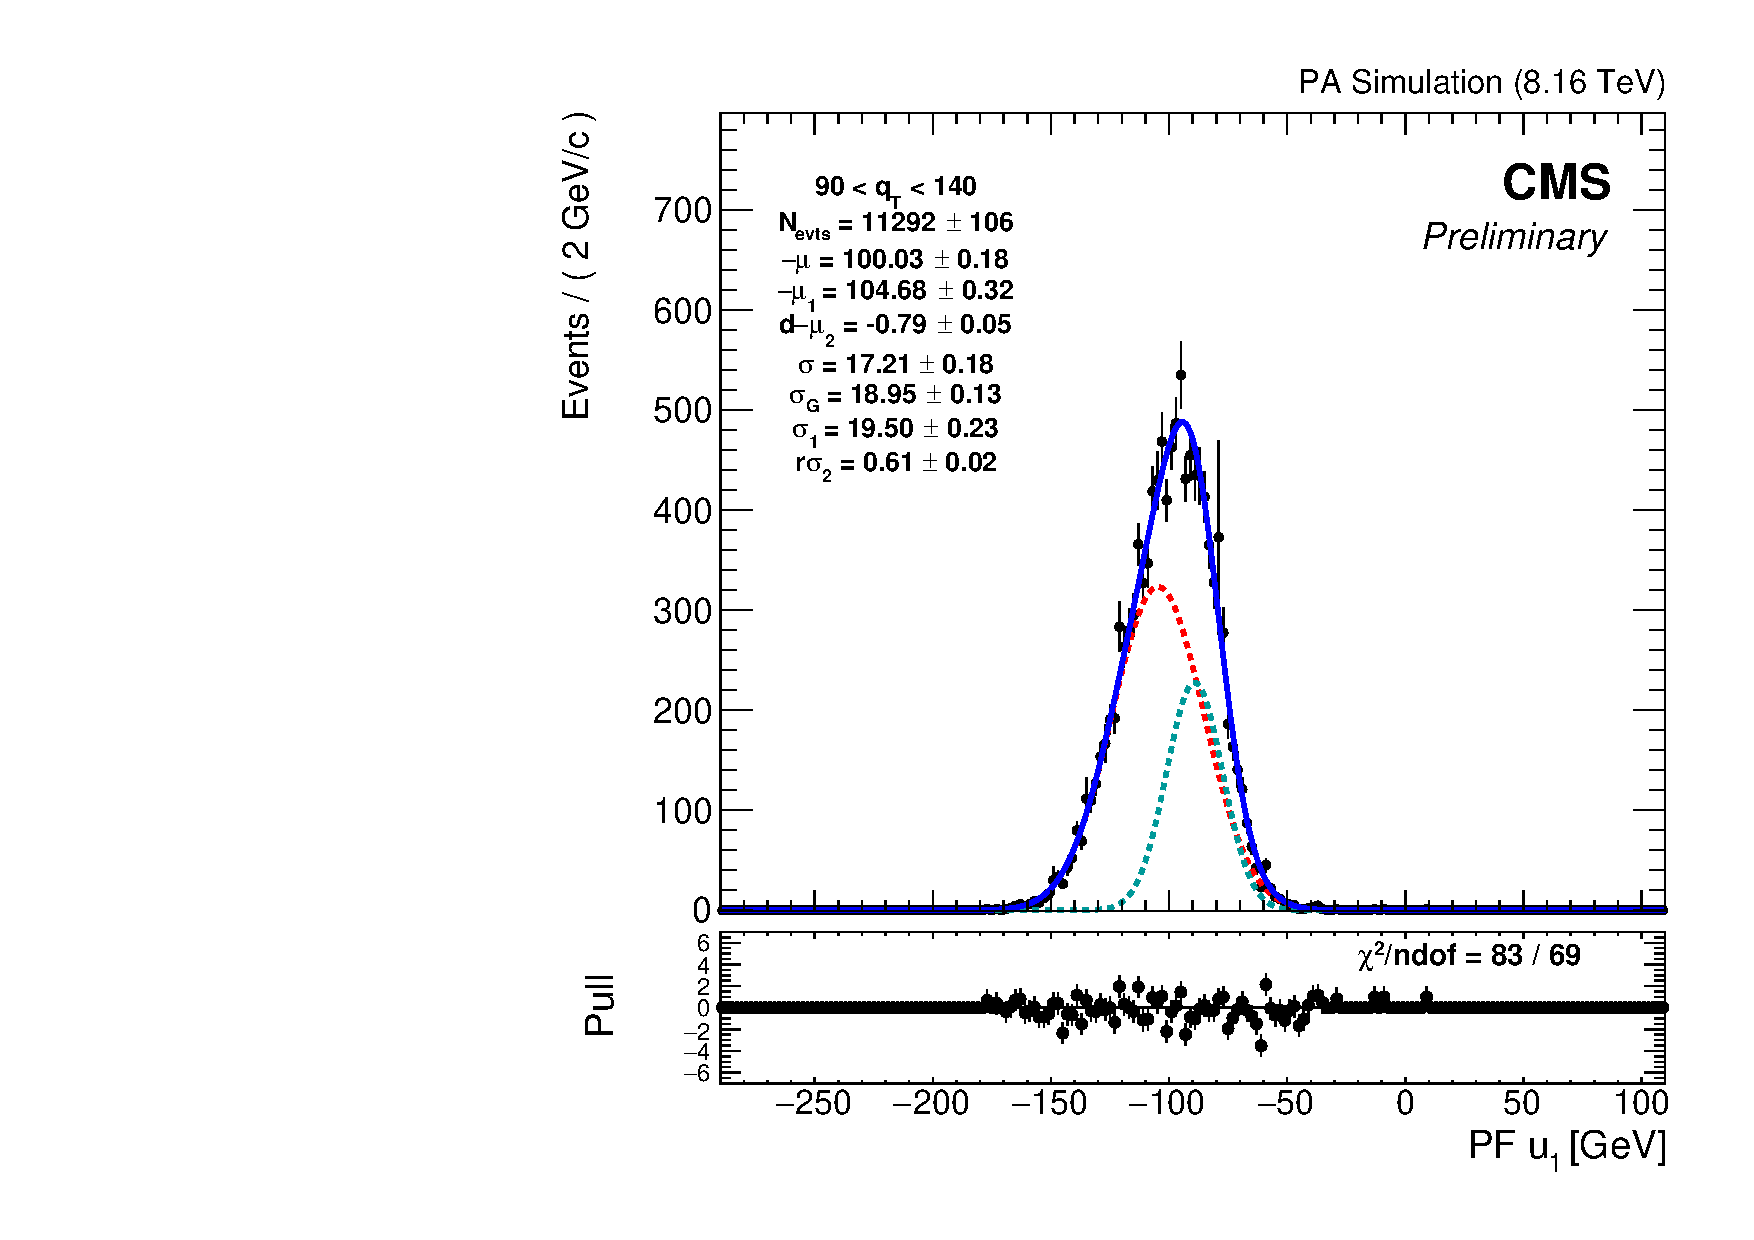
\includegraphics[width=0.4\textwidth]{Figures/WBoson/Analysis/Correction/Recoil/RecoilFits/MC/pfu1fit_29.pdf} \\
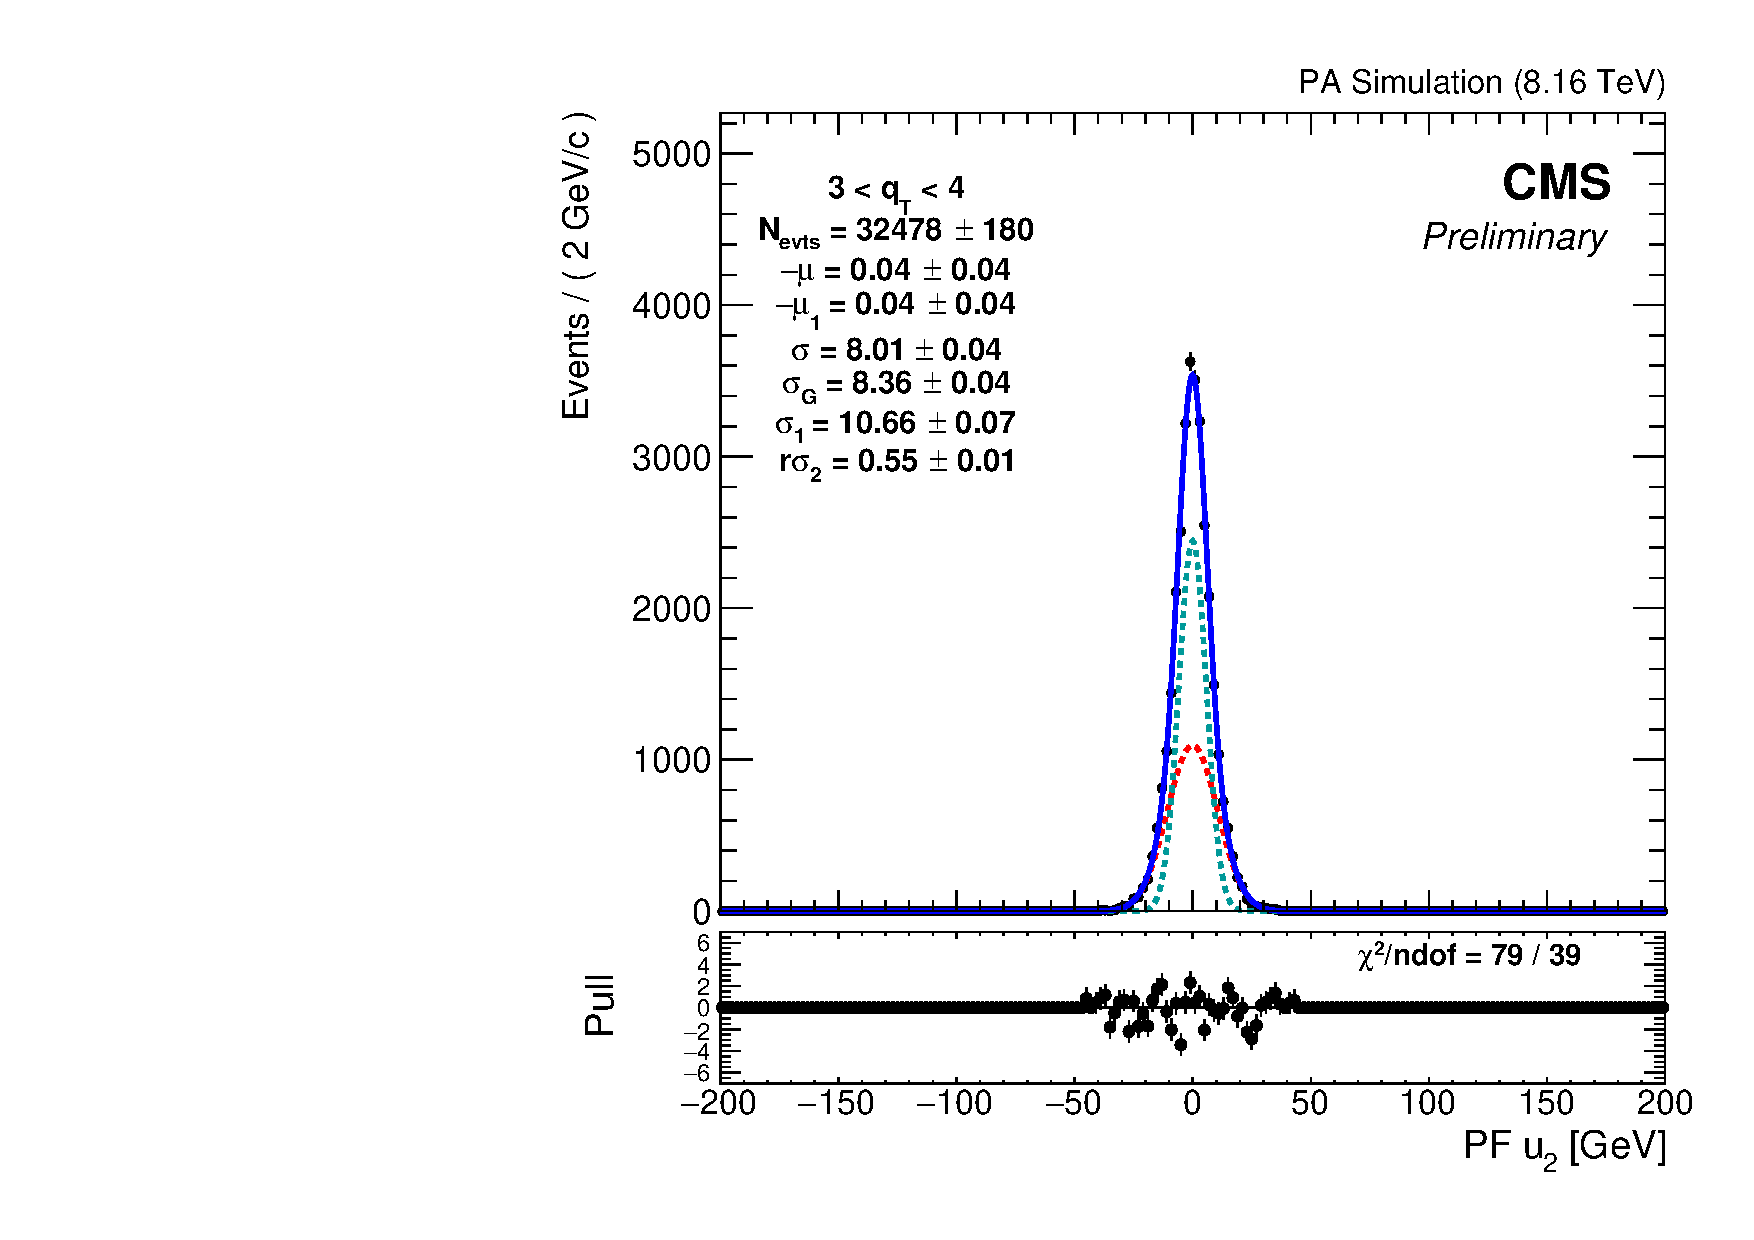
\includegraphics[width=0.4\textwidth]{Figures/WBoson/Analysis/Correction/Recoil/RecoilFits/MC/pfu2fit_2.pdf}
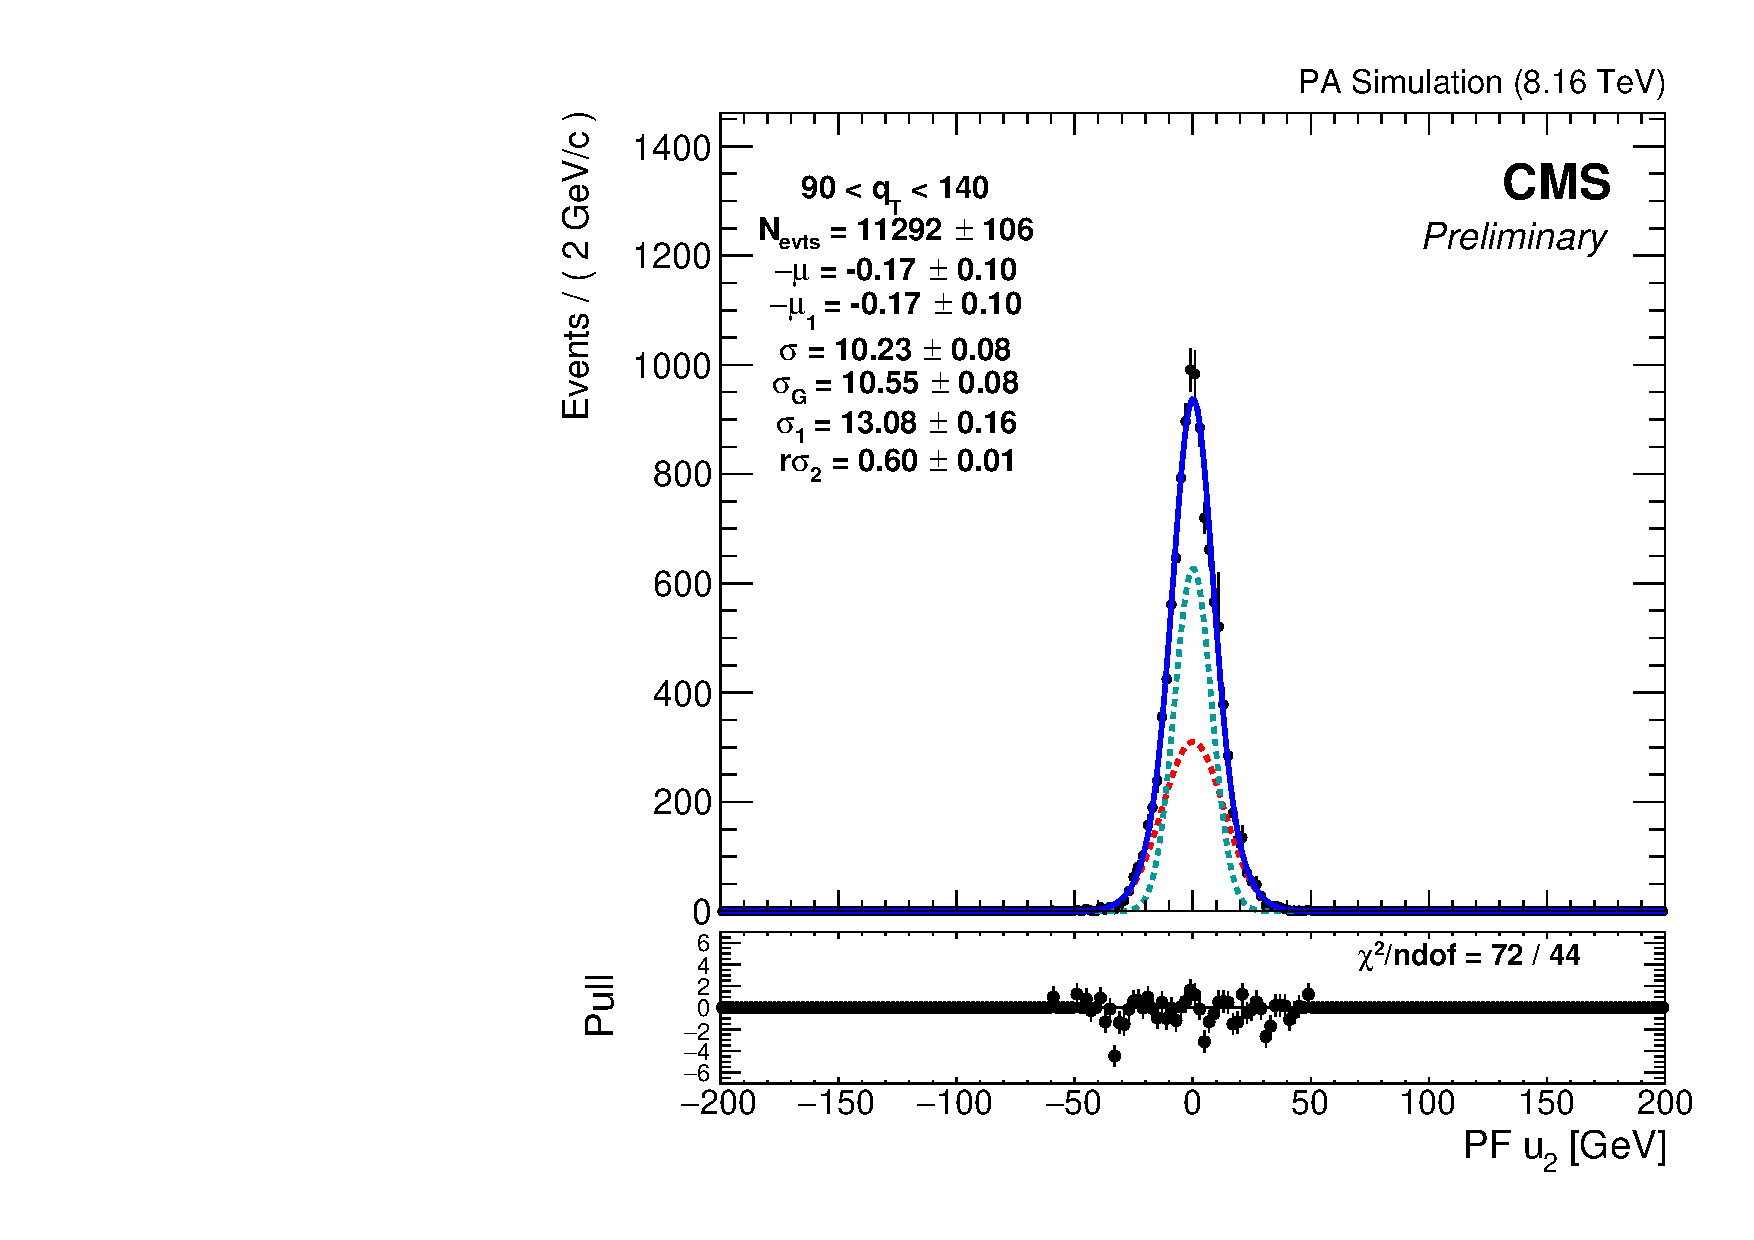
\includegraphics[width=0.4\textwidth]{Figures/WBoson/Analysis/Correction/Recoil/RecoilFits/MC/pfu2fit_29.pdf}
\caption{Distributions of the parallel (top) and perpendicular (bottom) components of the recoil in MC with the fits performed with the weighted sum of two Gaussian functions in \eq{eq:gaussFit}. The distributions are for the $q_{T}$
bins 3 GeV $< q_{T} <$ 4 GeV (left) and 90 GeV $< q_{T} <$ 140 GeV (right).}
\label{fig:RecoilFitsMC}
\end{center}
\end{figure}
 
 \clearpage
 
\subsubsection{Recoil scale}\label{sec:WBoson_Analysis_Rscale}

First, the $\mu_{1}$ and  $\mu_{2}$ average values of the parallel component of the recoil ($u_{1}$) is parametrised as a function of  $q_{T}$ from the fits shown in Figures ~\ref{fig:RecoilFitsData} and ~\ref{fig:RecoilFitsMC} in order to obtain an average recoil profile as a function $q_{T}$. The fit to the average recoil as a function of $q_{T}$ uses the following functional form: 

\begin{equation}\label{eq:equparparam} 
-\mu_{1,2}(q_{T}) = (c_{0} + c_{1}q_{T})(1 + erf(\alpha q_{T}^{\beta}))
\end{equation}

The fits for the $\mu_{1}$ and  $\mu_{2}$ values of parallel component of the recoil versus $q_{T}$ for data and MC Z samples are shown in Figures ~\ref{fig:figU1RecoilScaleFit_data} and ~\ref{fig:figU1RecoilScaleFit_MC} respectively. In addition, the weighted average of $\mu_{1}$ and  $\mu_{2}$, $\mu = f \cdot \mu_{1} + (1 - f) \cdot \mu_{2}$, is also shown. The difference between data and MC as a function of $q_{T}$ is used on an event by event basis to correct the scale of the recoil in MC as described in \sect{recoilCorr}.

\begin{figure}
\begin{center}
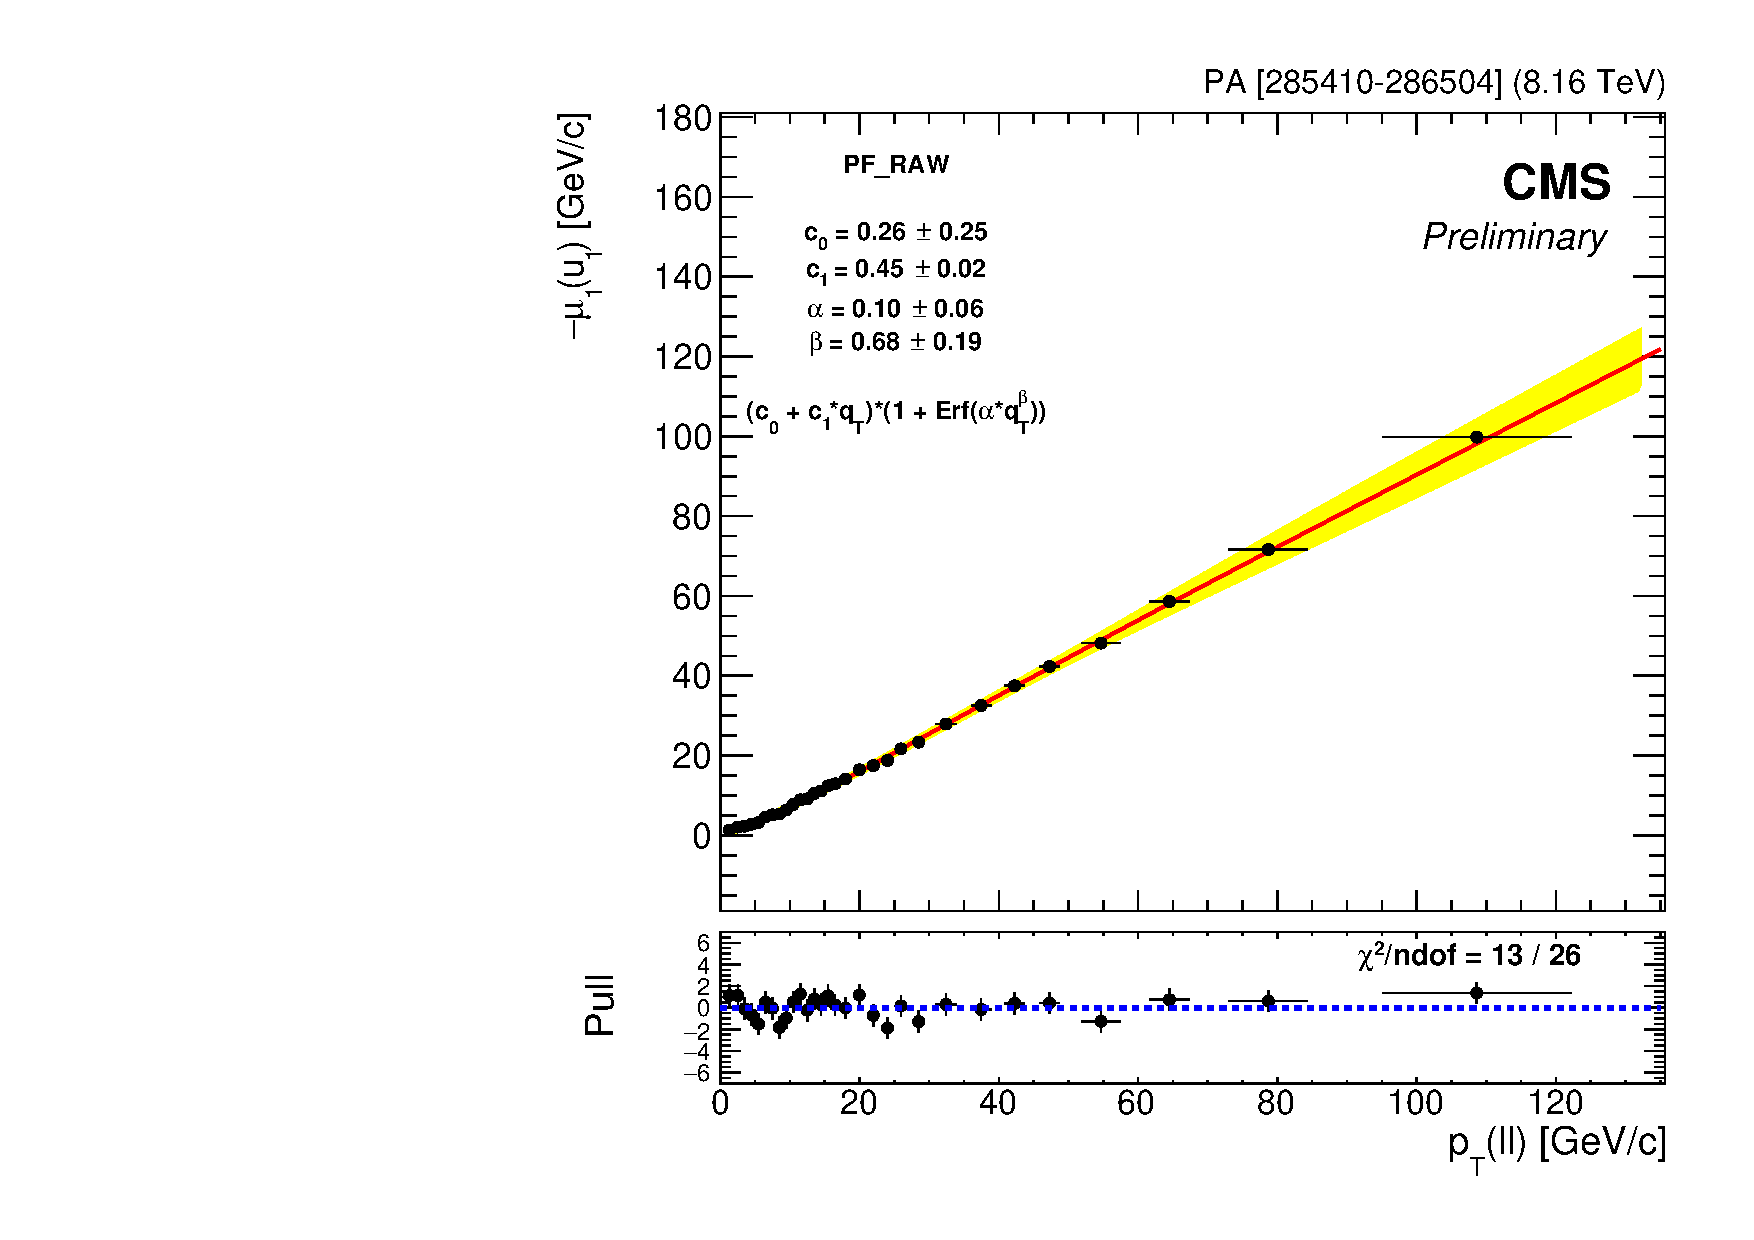
\includegraphics[width=0.4\textwidth]{Figures/WBoson/Analysis/Correction/Recoil/RecoilFitsqT/Data/fitPFu1mean1.pdf}
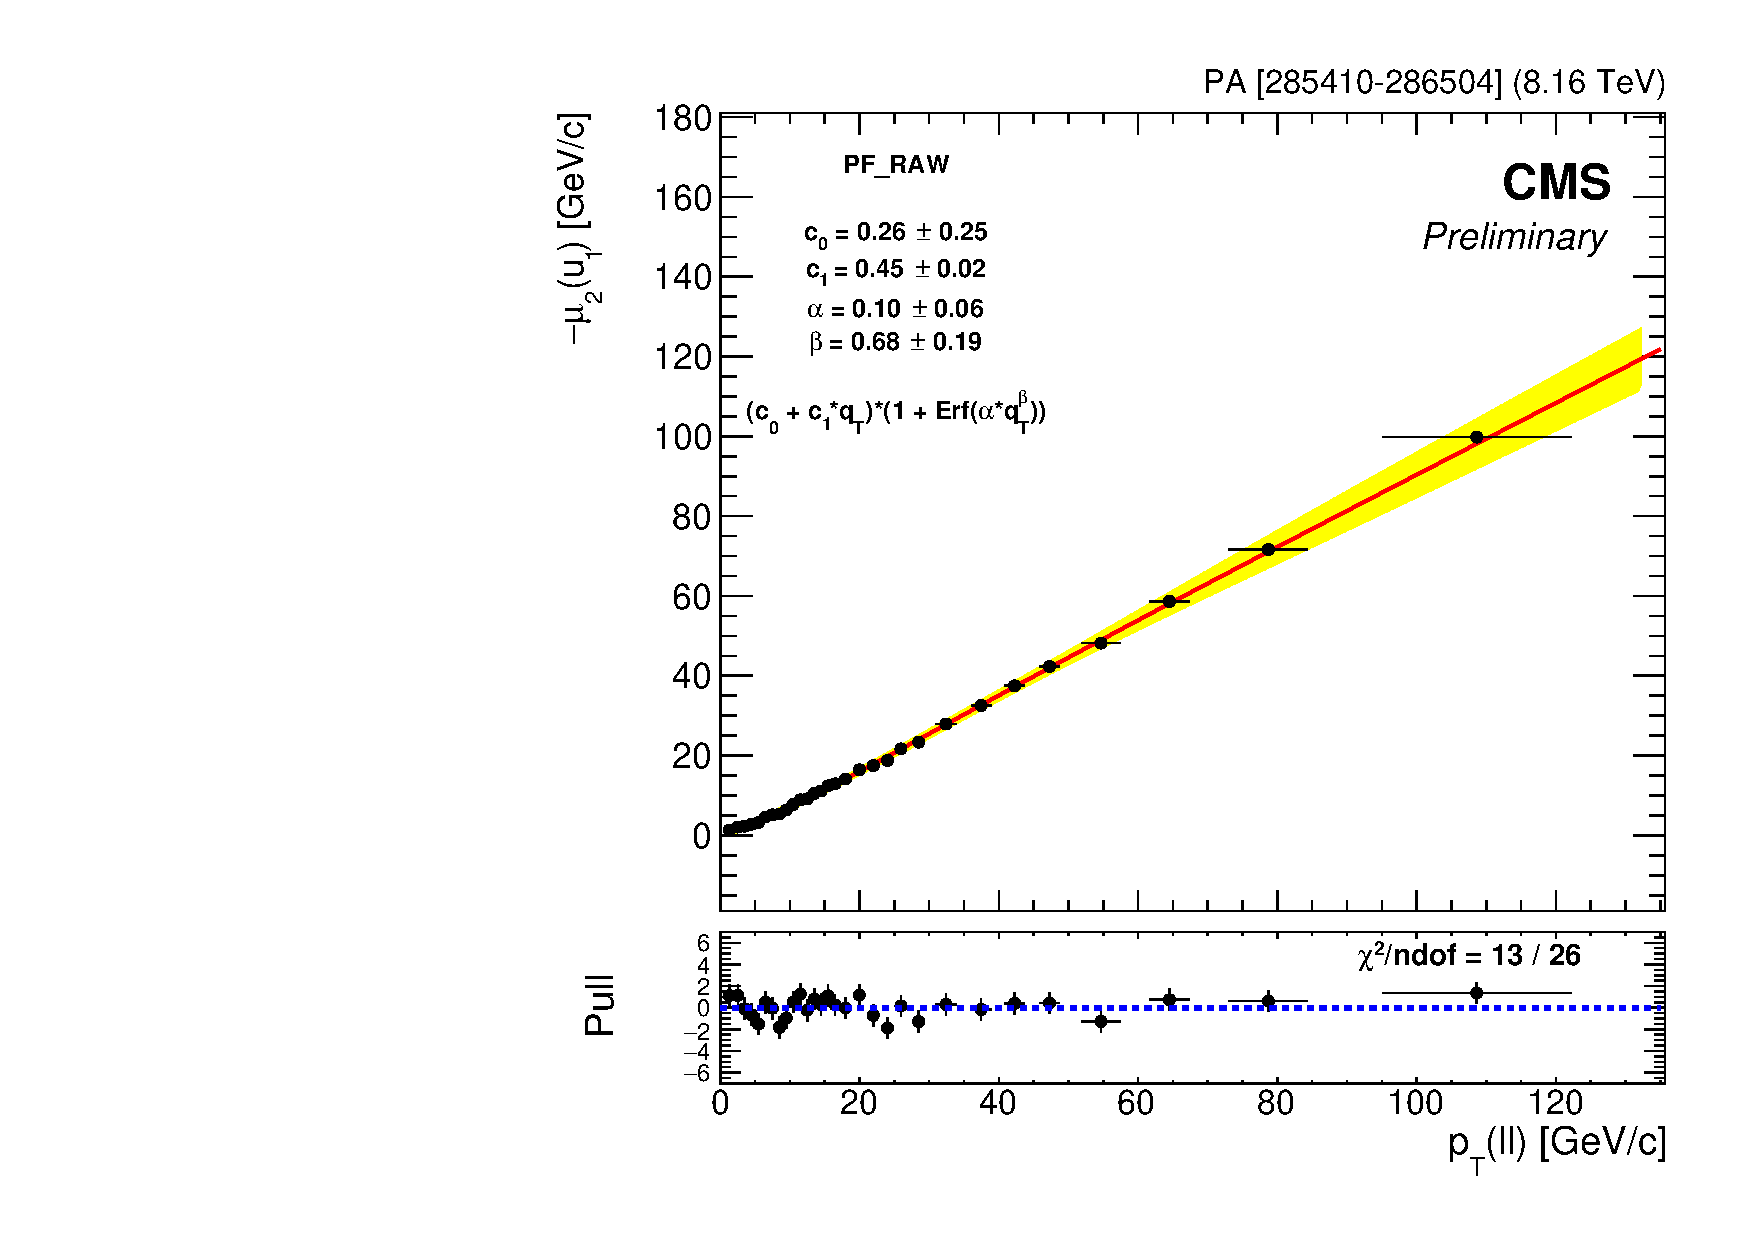
\includegraphics[width=0.4\textwidth]{Figures/WBoson/Analysis/Correction/Recoil/RecoilFitsqT/Data/fitPFu1mean2.pdf} \\
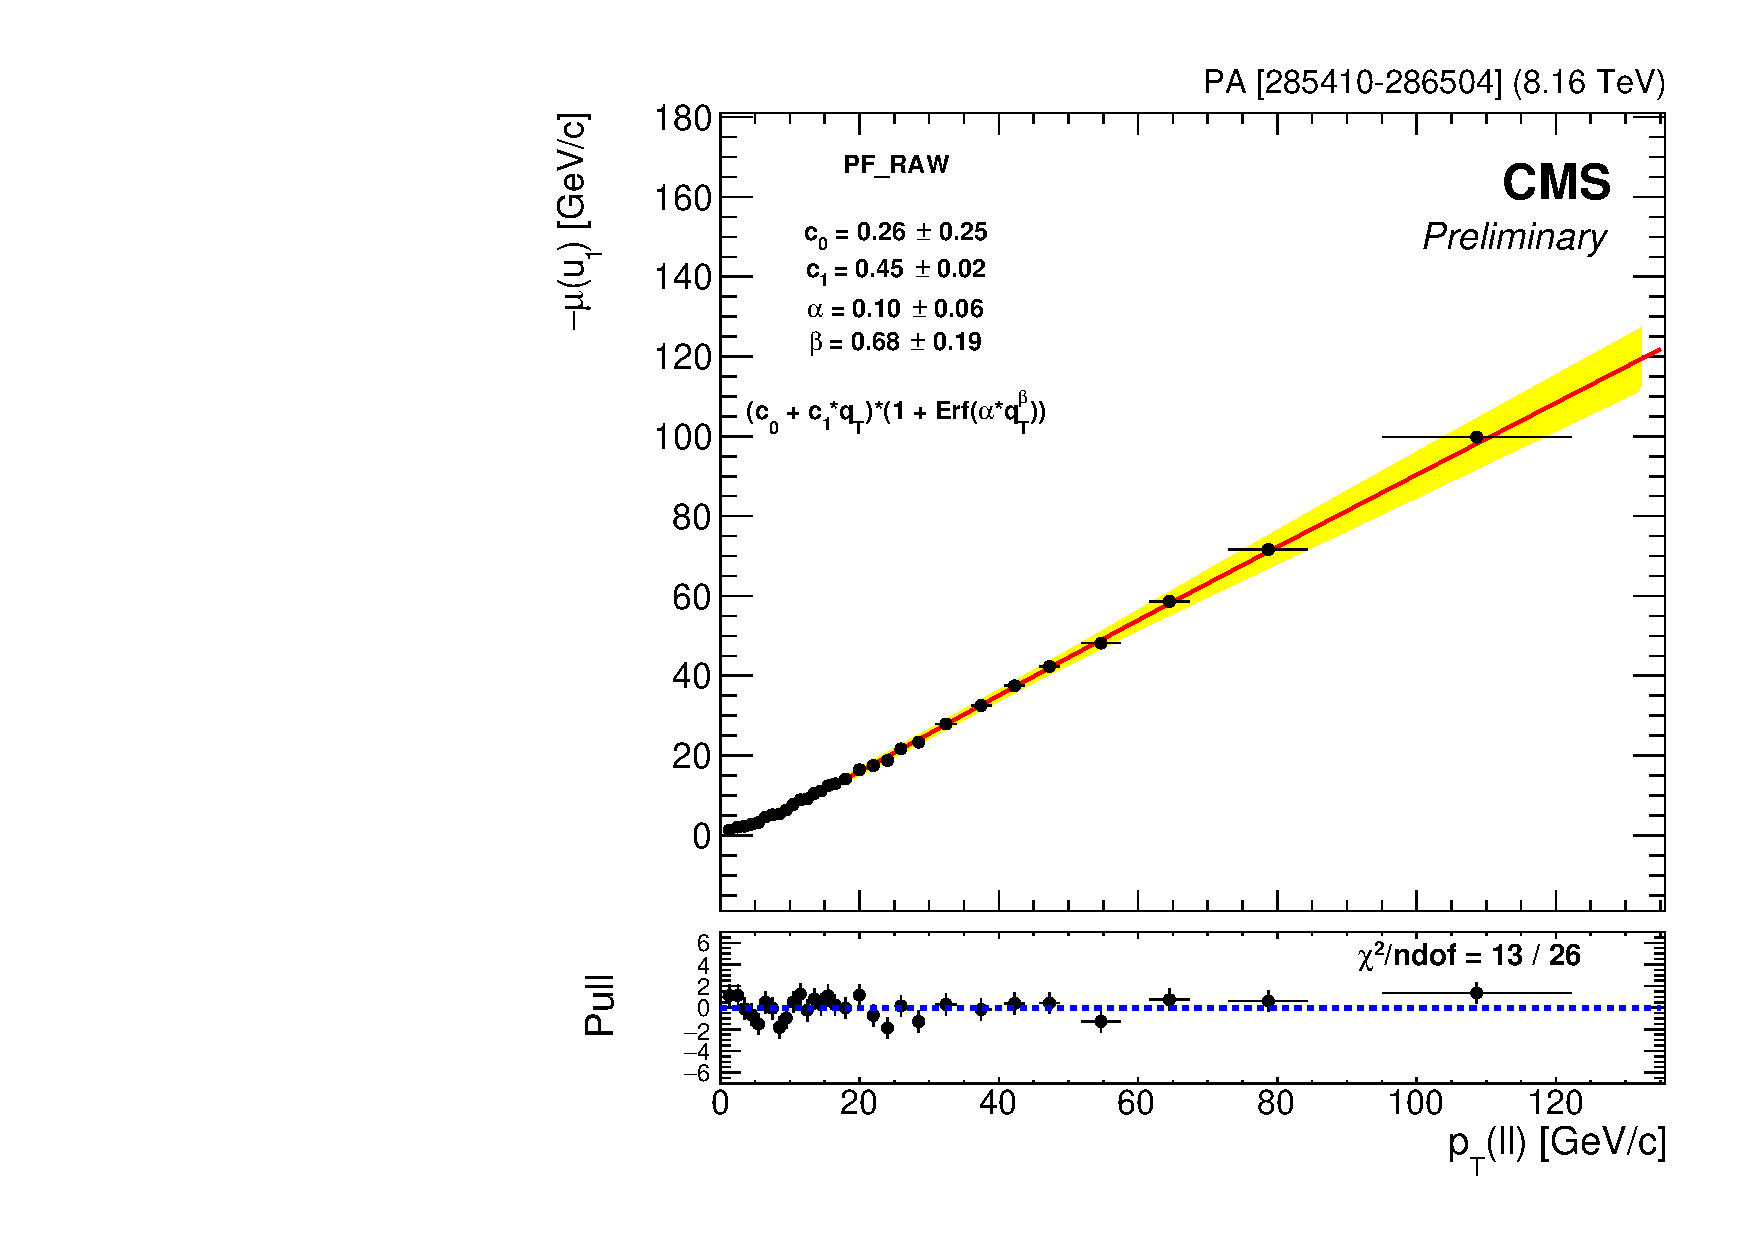
\includegraphics[width=0.4\textwidth]{Figures/WBoson/Analysis/Correction/Recoil/RecoilFitsqT/Data/fitPFu1mean.pdf}
\caption{Fits for the $\mu_{1}$,  $\mu_{2}$ (top) and $\mu$ (bottom) values of parallel component of the recoil versus $q_{T}$ for the data Z boson dimuon sample.}
\label{fig:figU1RecoilScaleFit_data}
\end{center}
\end{figure}

\begin{figure}
\begin{center}
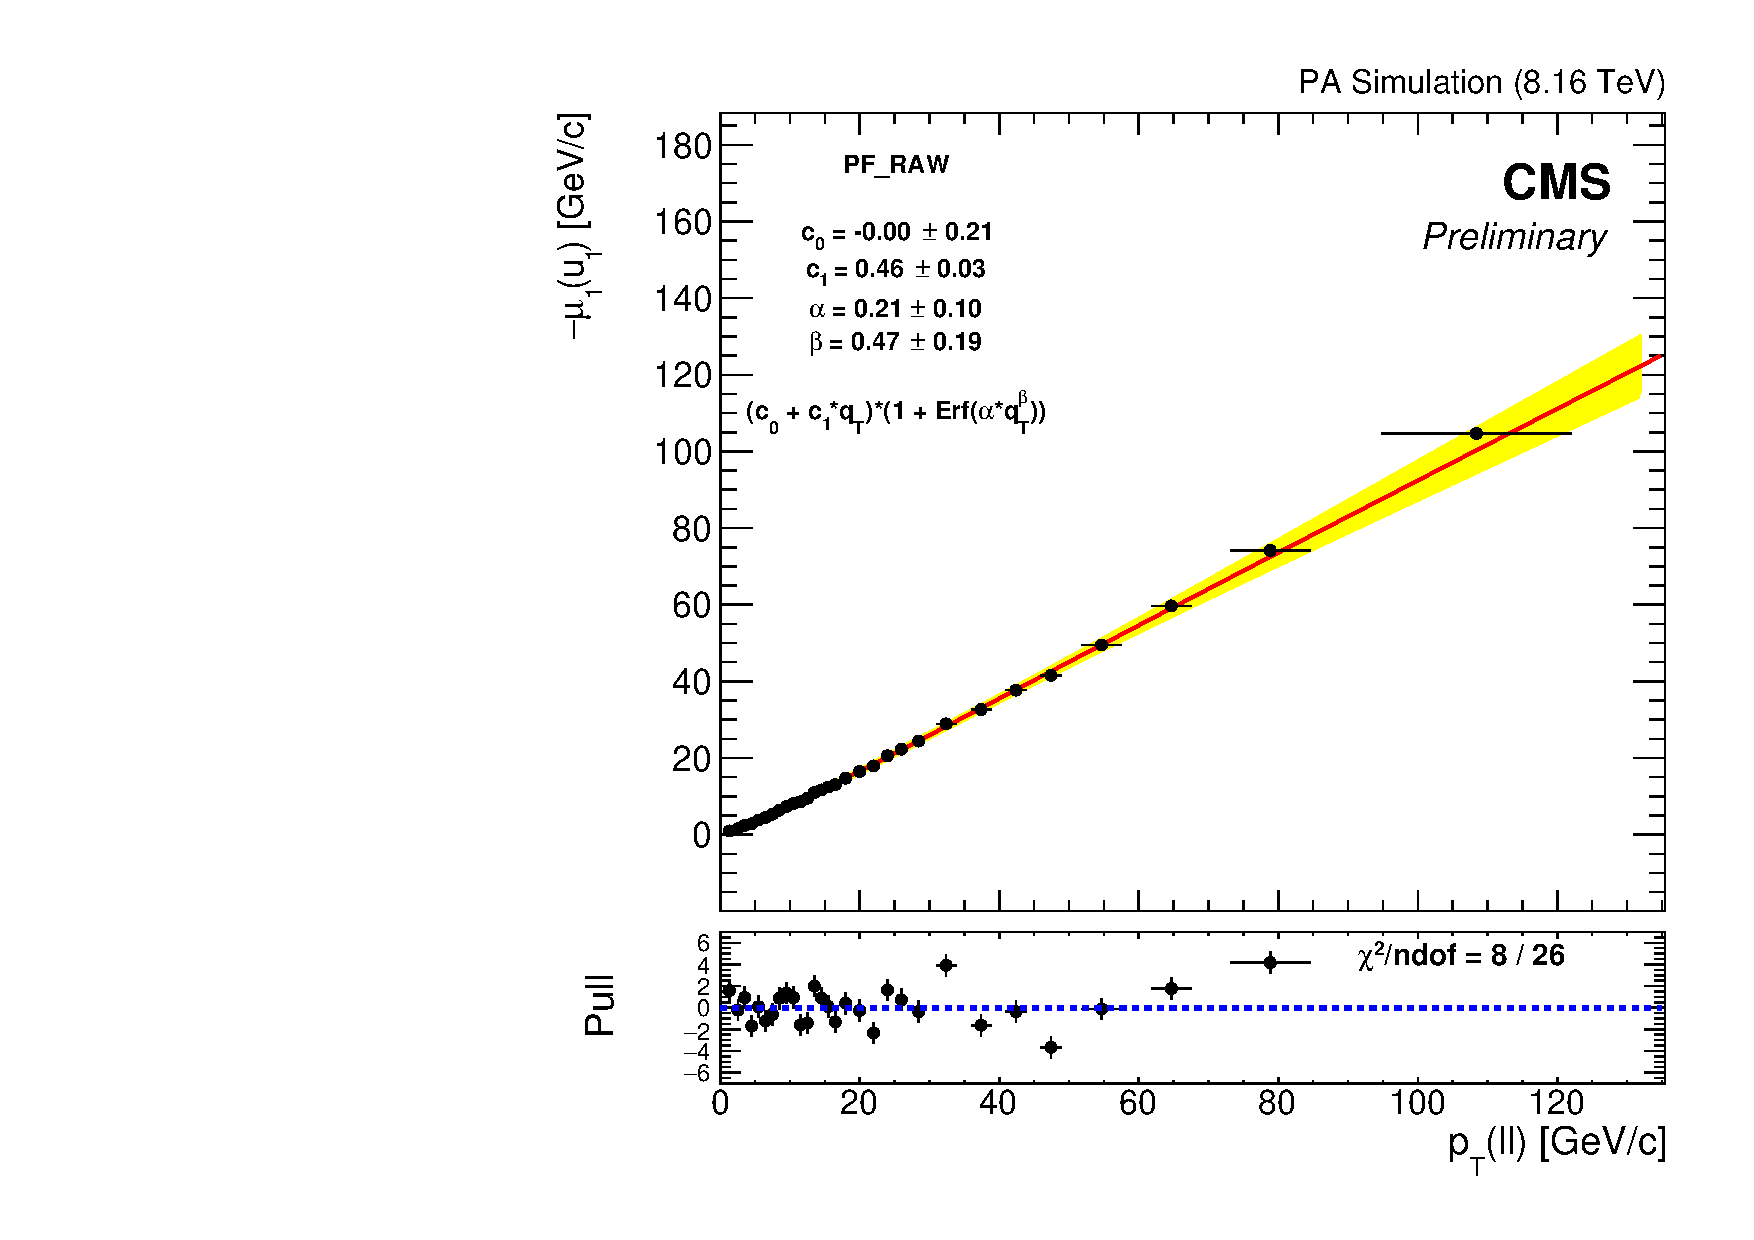
\includegraphics[width=0.4\textwidth]{Figures/WBoson/Analysis/Correction/Recoil/RecoilFitsqT/MC/fitPFu1mean1.pdf}
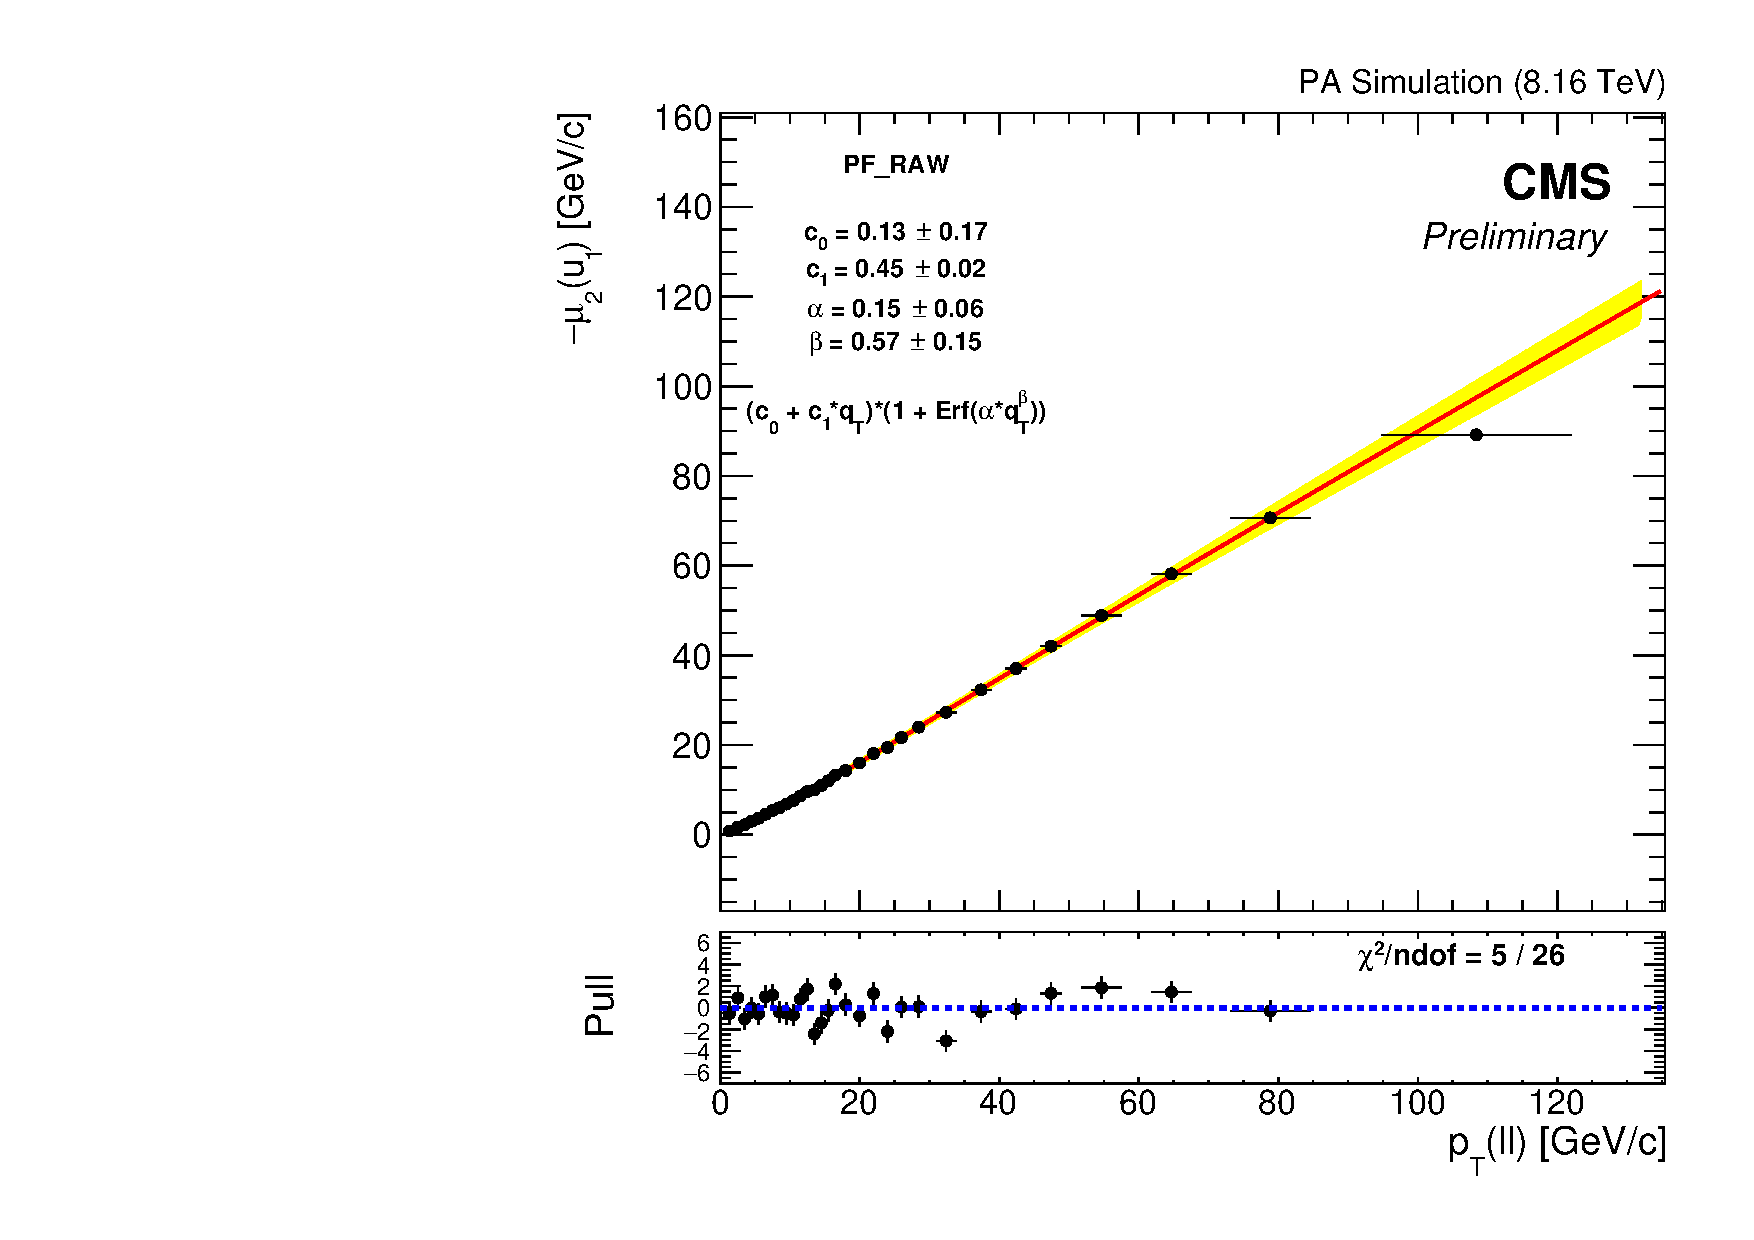
\includegraphics[width=0.4\textwidth]{Figures/WBoson/Analysis/Correction/Recoil/RecoilFitsqT/MC/fitPFu1mean2.pdf} \\
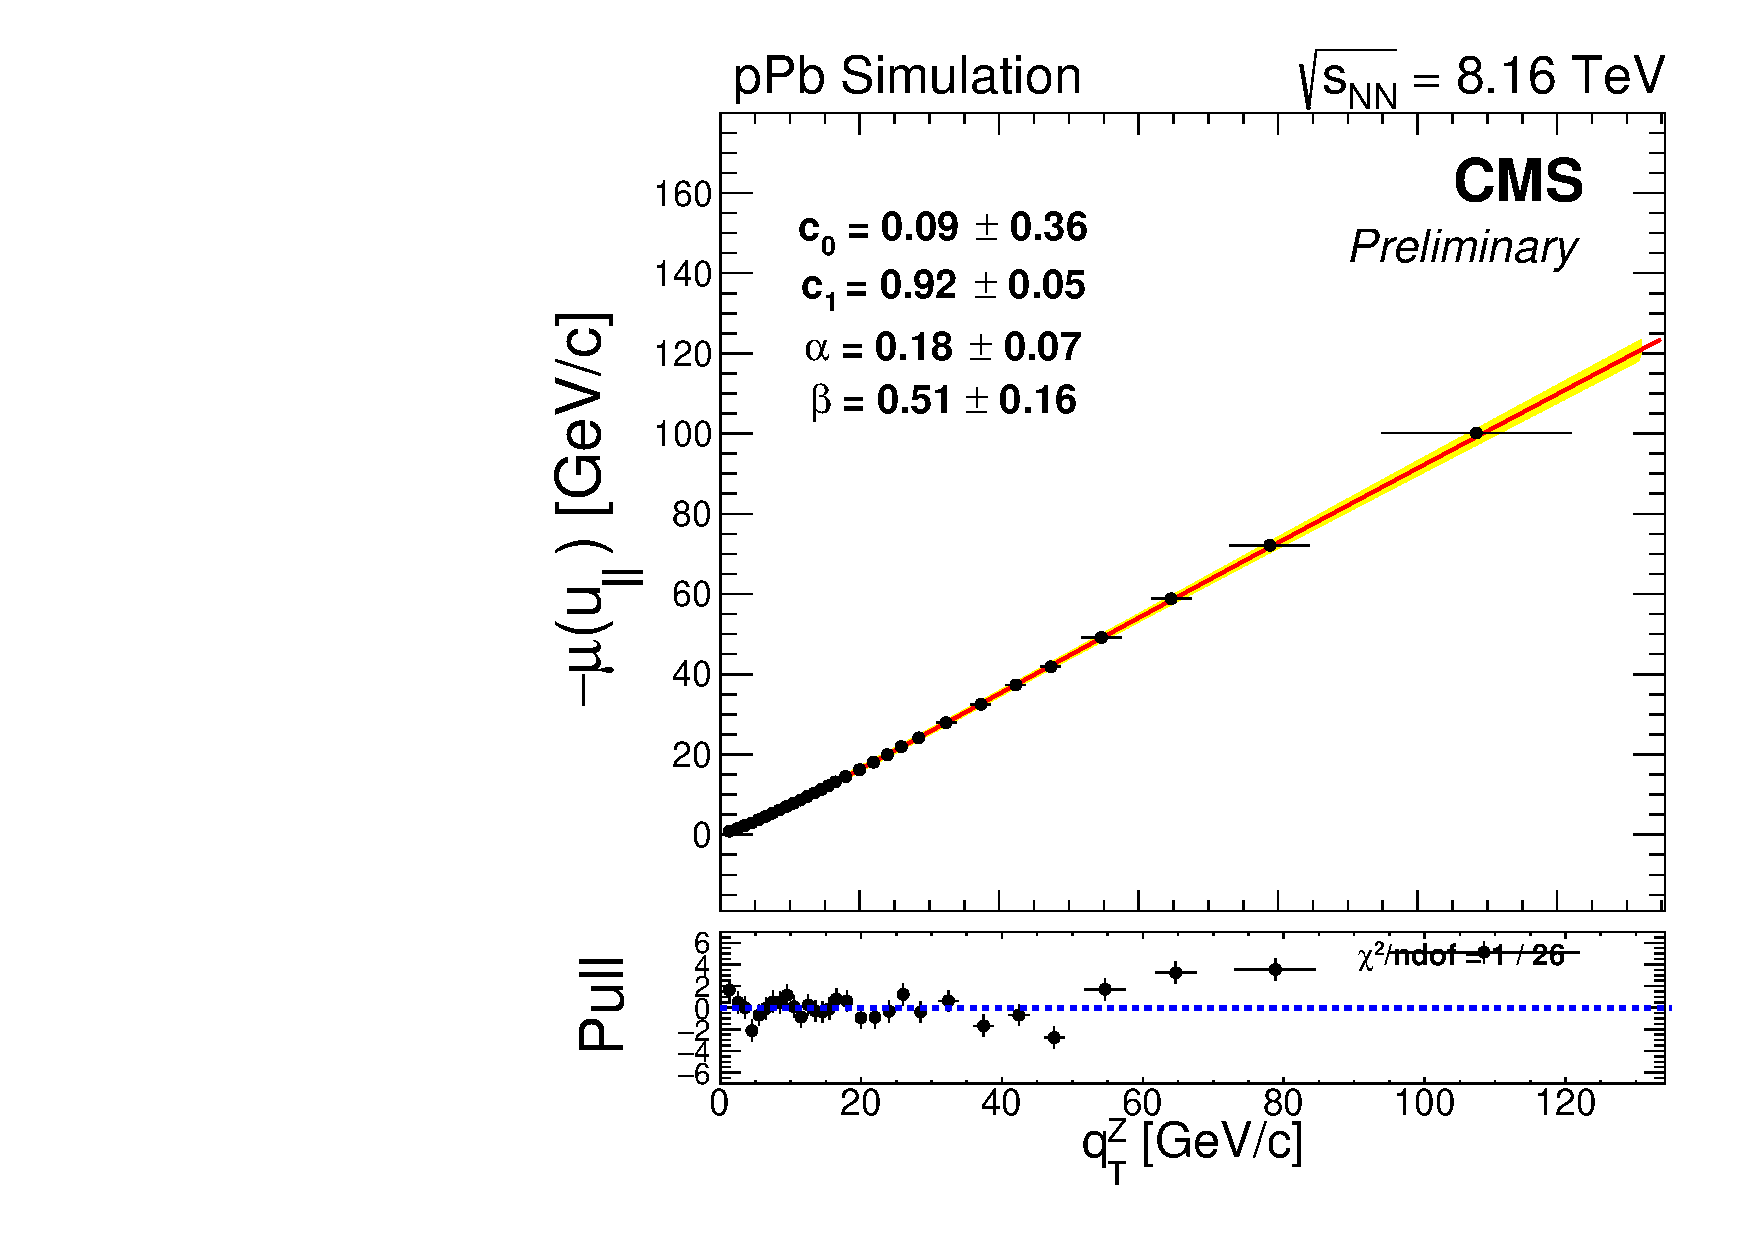
\includegraphics[width=0.4\textwidth]{Figures/WBoson/Analysis/Correction/Recoil/RecoilFitsqT/MC/fitPFu1mean.pdf}
\caption{Fits for the $\mu_{1}$,  $\mu_{2}$ (top) and $\mu$ (bottom) values of parallel component of the recoil versus $q_{T}$ for the MC Z boson dimuon sample.}
\label{fig:figU1RecoilScaleFit_MC}
\end{center}
\end{figure}

The $\mu_{1}$ and  $\mu_{2}$ average values of the perpendicular component of the recoil ($u_{2}$) versus $q_{T}$ for data and MC Z samples, are fitted with a constant function ($c_{0}$), and the results are shown in Figures ~\ref{fig:figU2RecoilScaleFit_data} and ~\ref{fig:figU2RecoilScaleFit_MC}. Also, the weighted average of $\mu_{1}$ and  $\mu_{2}$ is shown. One observe that the average perpendicular component is consistent with zero, and so, it is set to zero in the correction procedure.

\begin{figure}
\begin{center}
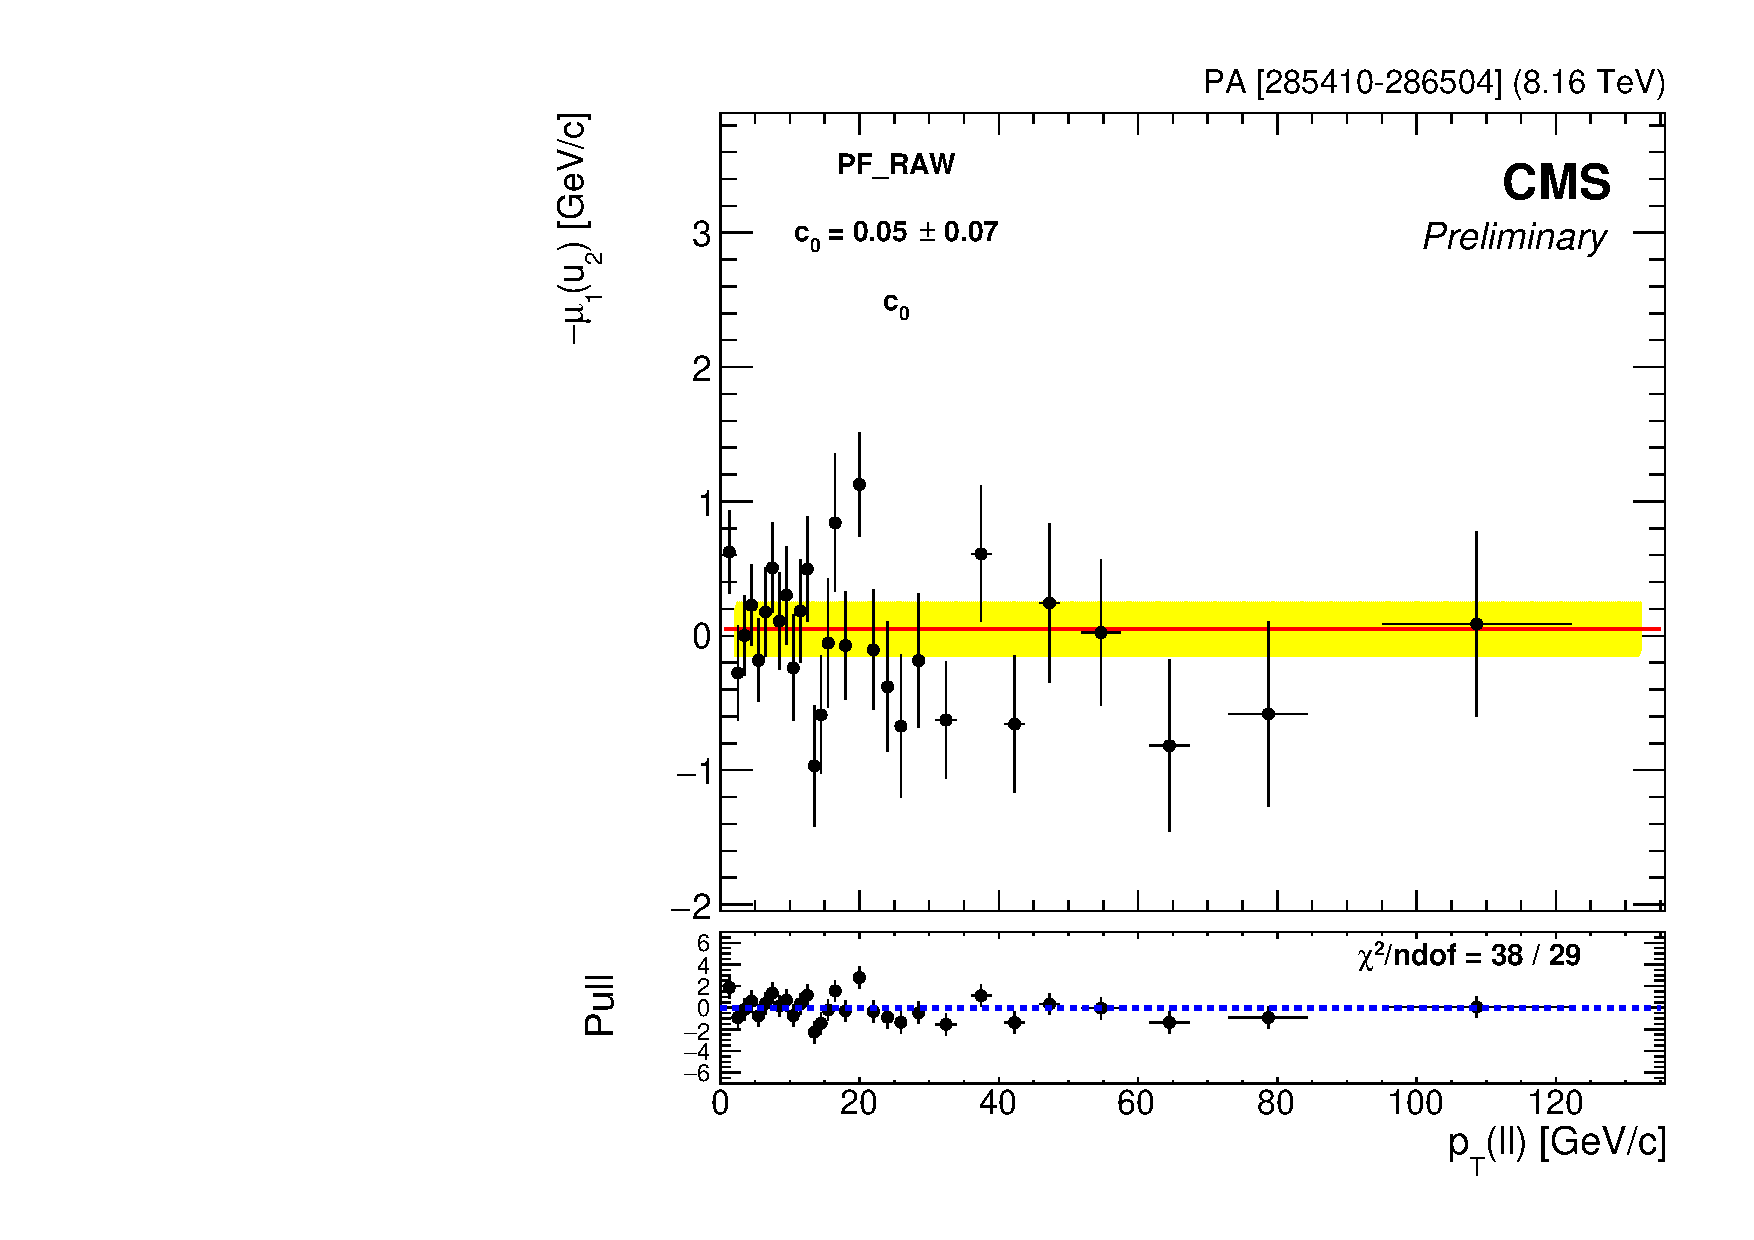
\includegraphics[width=0.4\textwidth]{Figures/WBoson/Analysis/Correction/Recoil/RecoilFitsqT/Data/fitPFu2mean1.pdf}
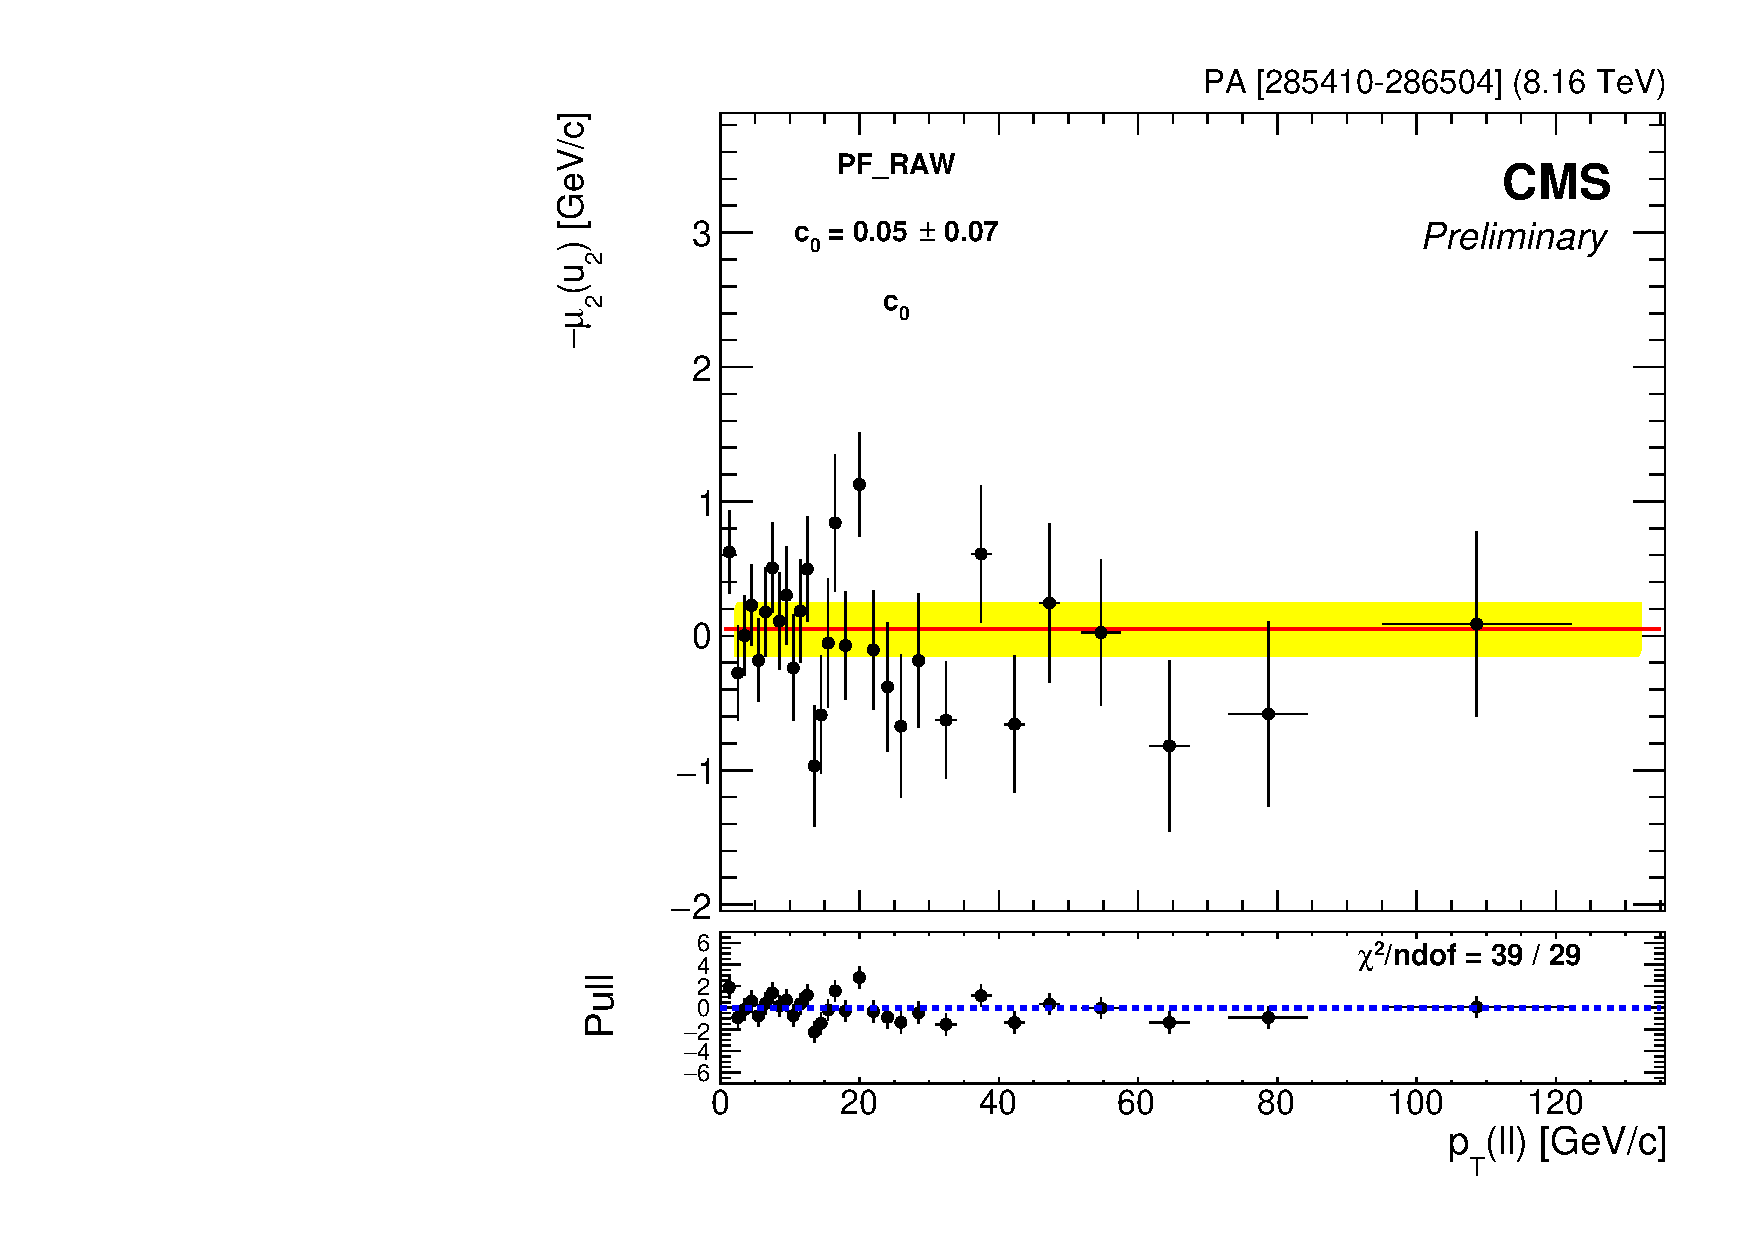
\includegraphics[width=0.4\textwidth]{Figures/WBoson/Analysis/Correction/Recoil/RecoilFitsqT/Data/fitPFu2mean2.pdf} \\
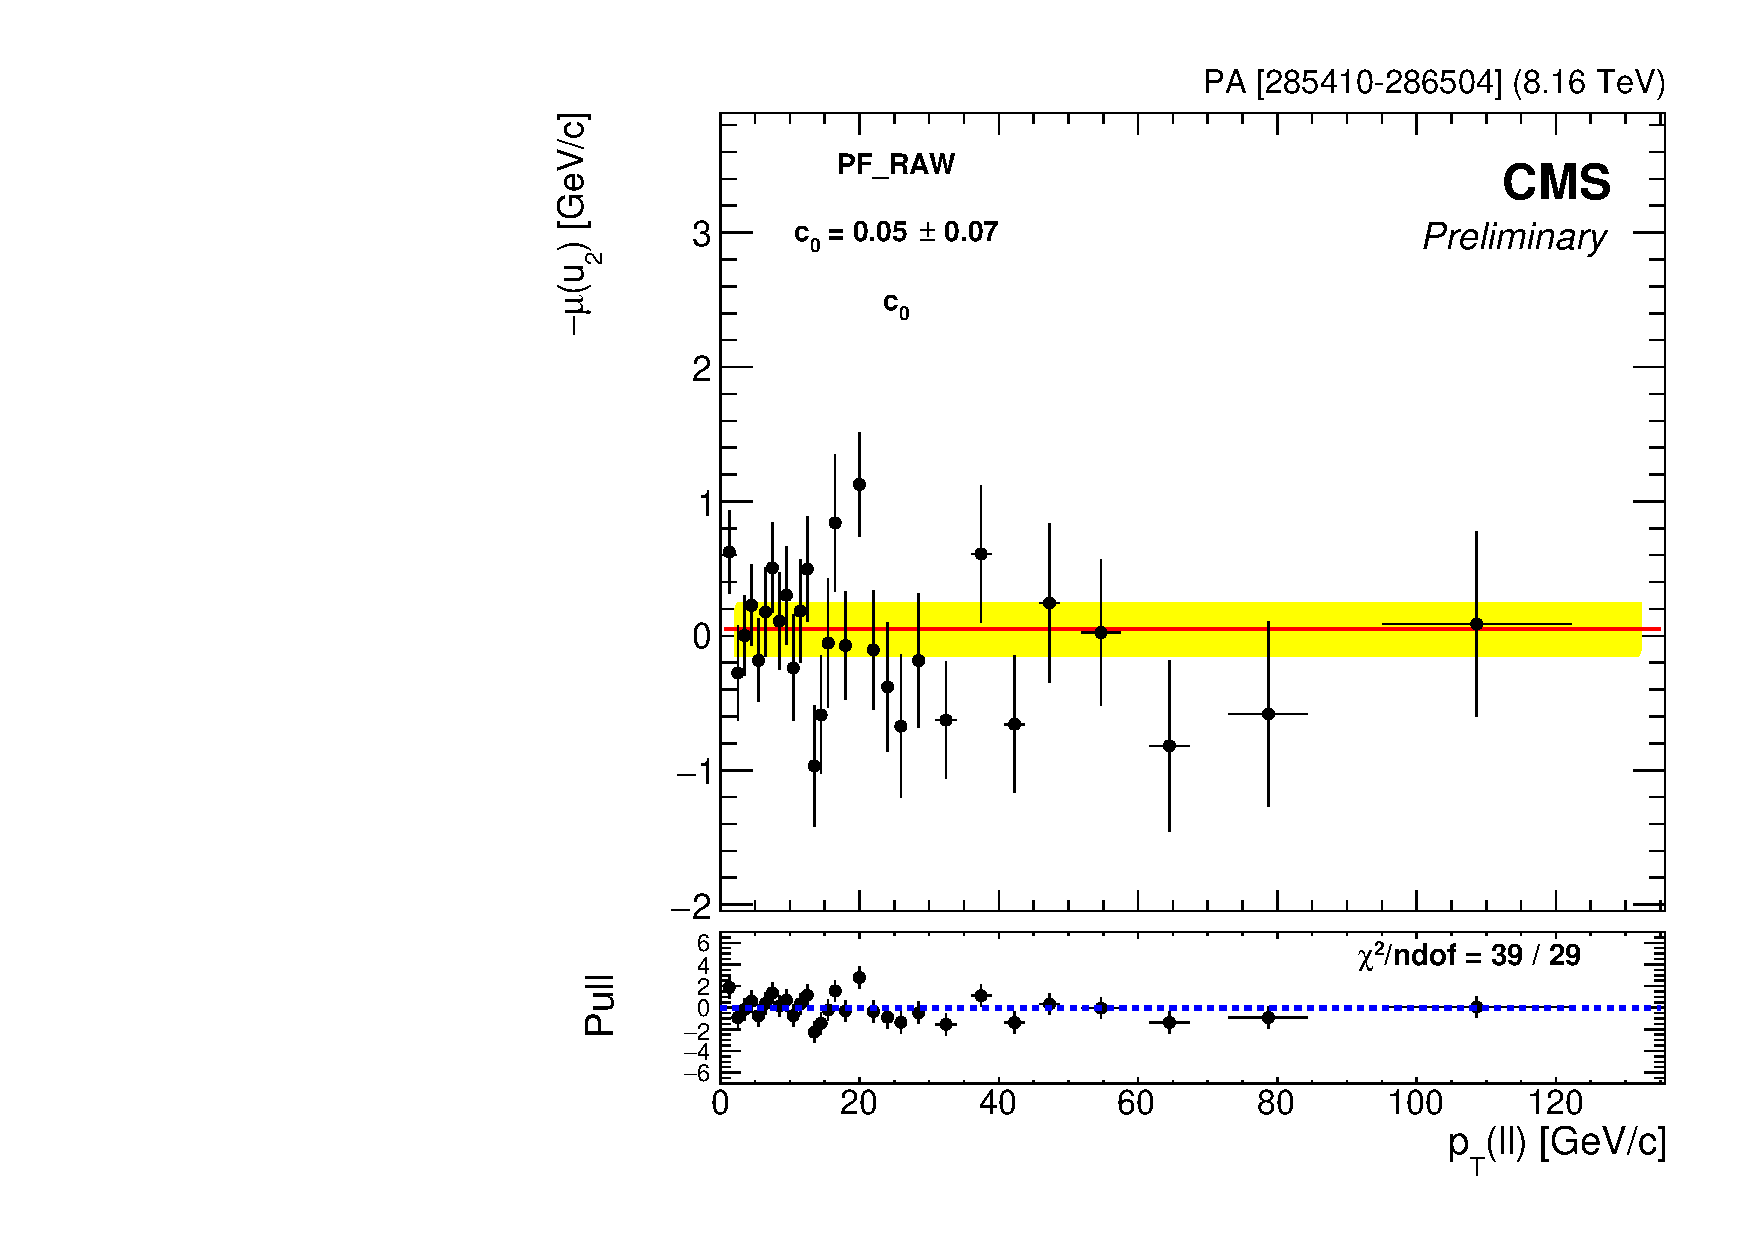
\includegraphics[width=0.4\textwidth]{Figures/WBoson/Analysis/Correction/Recoil/RecoilFitsqT/Data/fitPFu2mean.pdf}
\caption{Fits for the $\mu_{1}$,  $\mu_{2}$ (top) and $\mu$ (bottom) values of perpendicular component of the recoil versus $q_{T}$ for the data Z boson dimuon sample.}
\label{fig:figU2RecoilScaleFit_data}
\end{center}
\end{figure}

\begin{figure}
\begin{center}
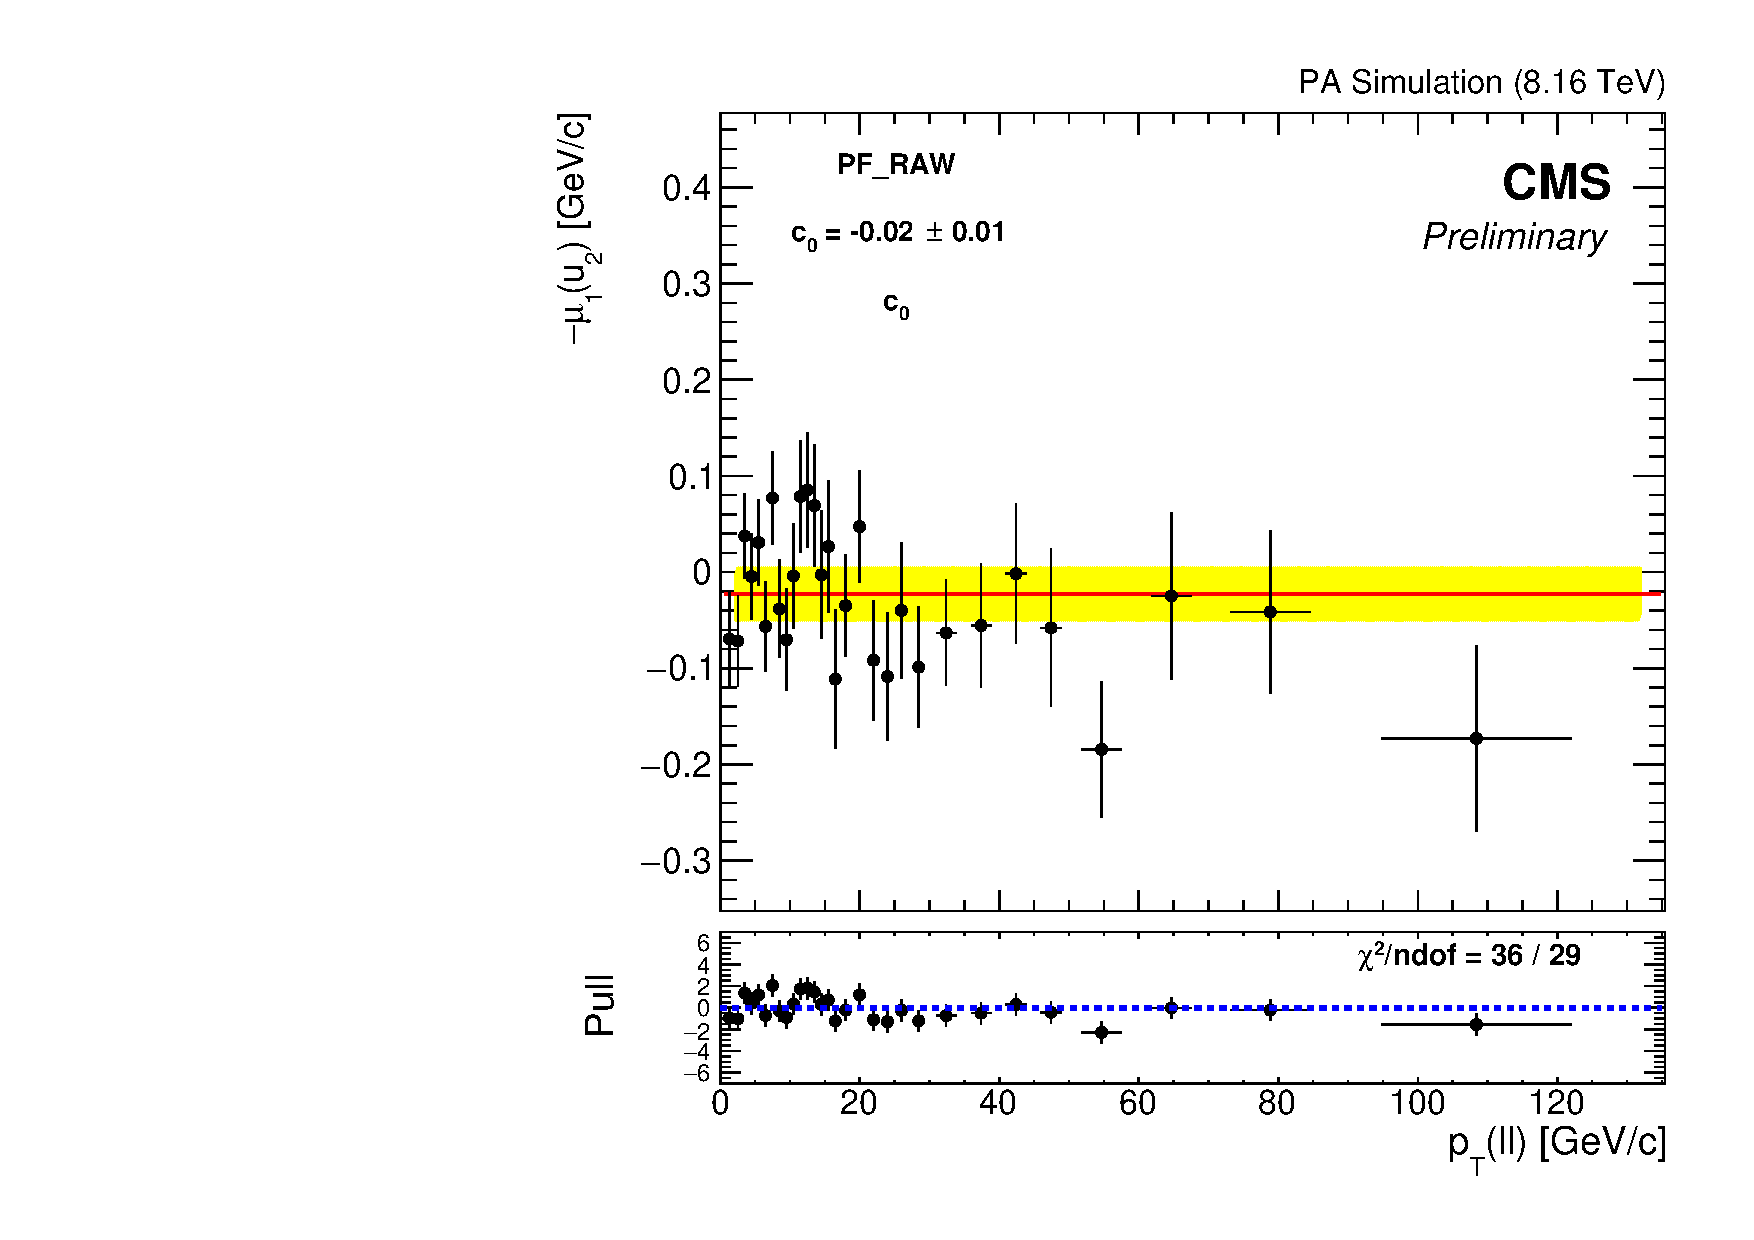
\includegraphics[width=0.4\textwidth]{Figures/WBoson/Analysis/Correction/Recoil/RecoilFitsqT/MC/fitPFu2mean1.pdf}
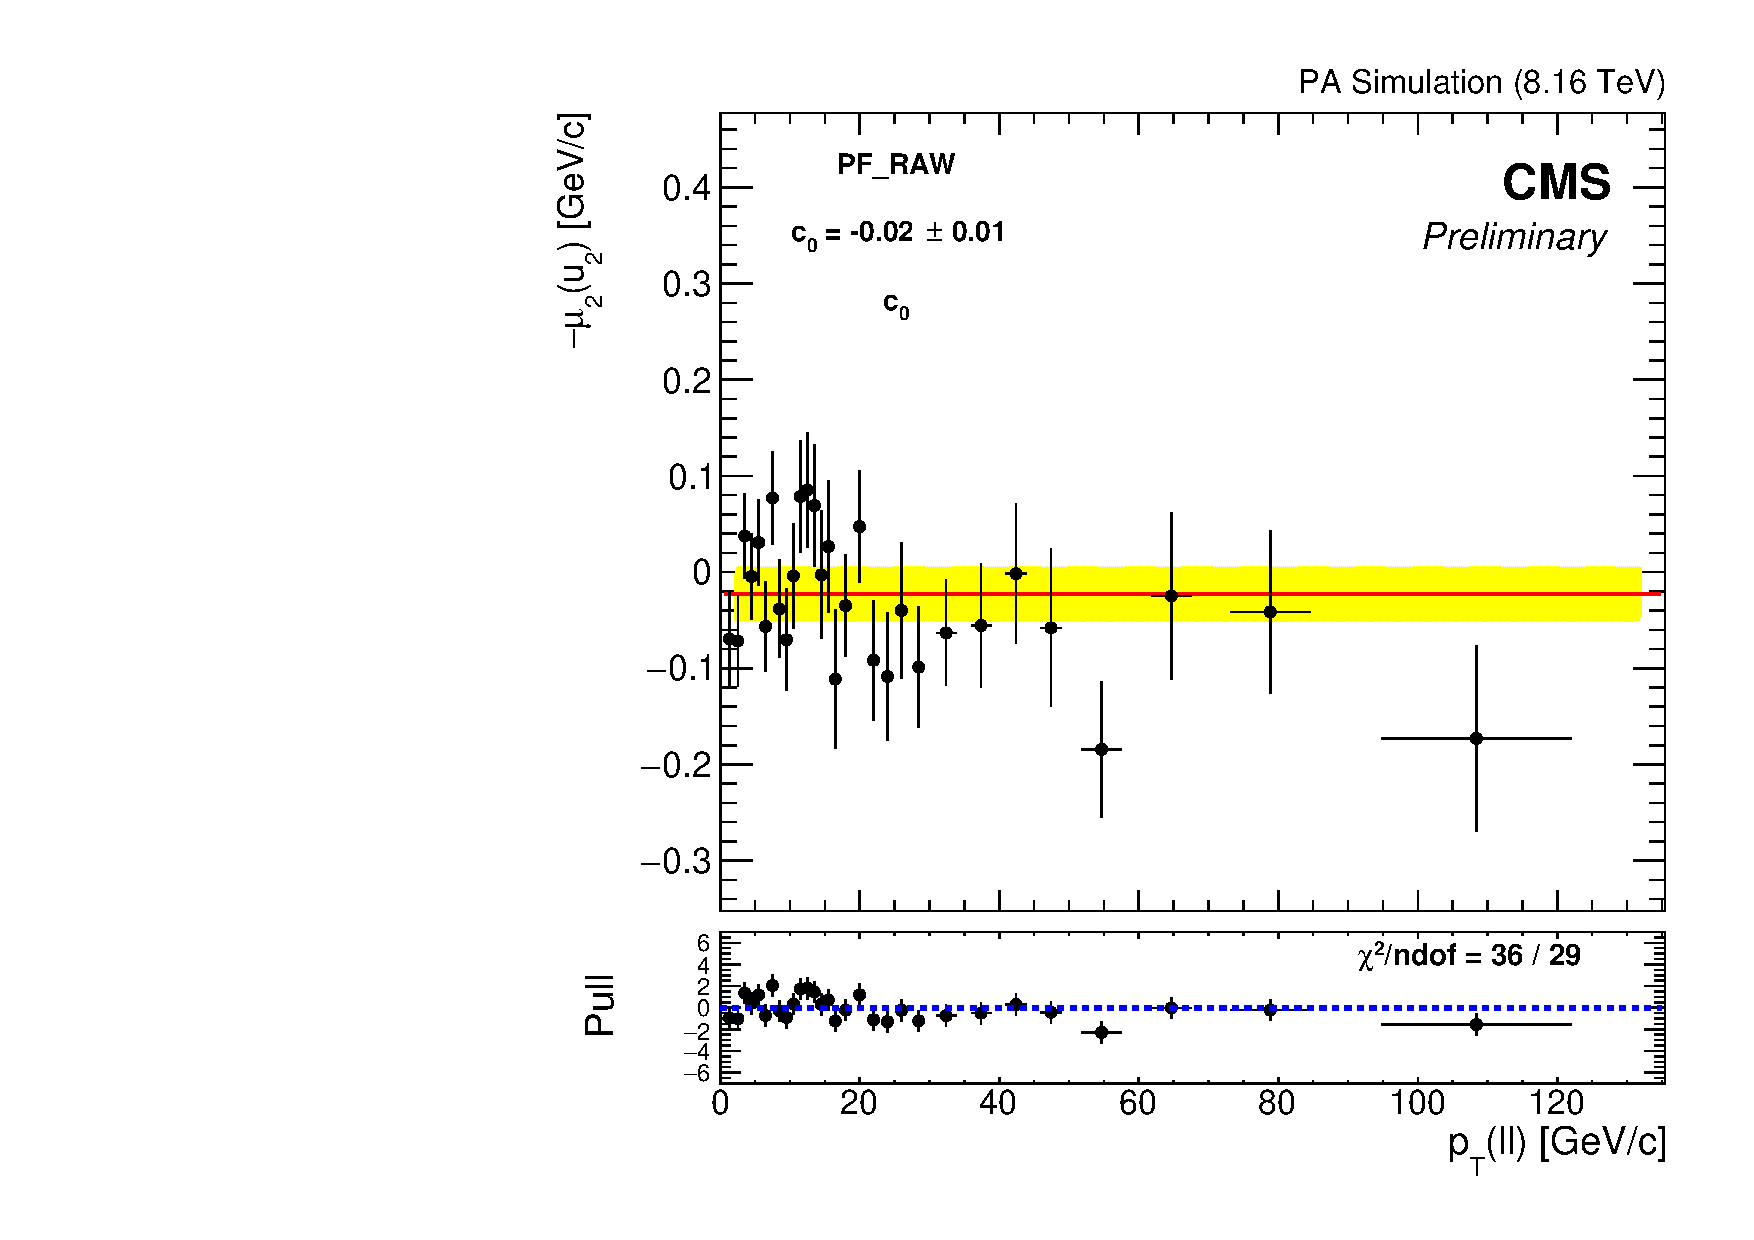
\includegraphics[width=0.4\textwidth]{Figures/WBoson/Analysis/Correction/Recoil/RecoilFitsqT/MC/fitPFu2mean2.pdf} \\
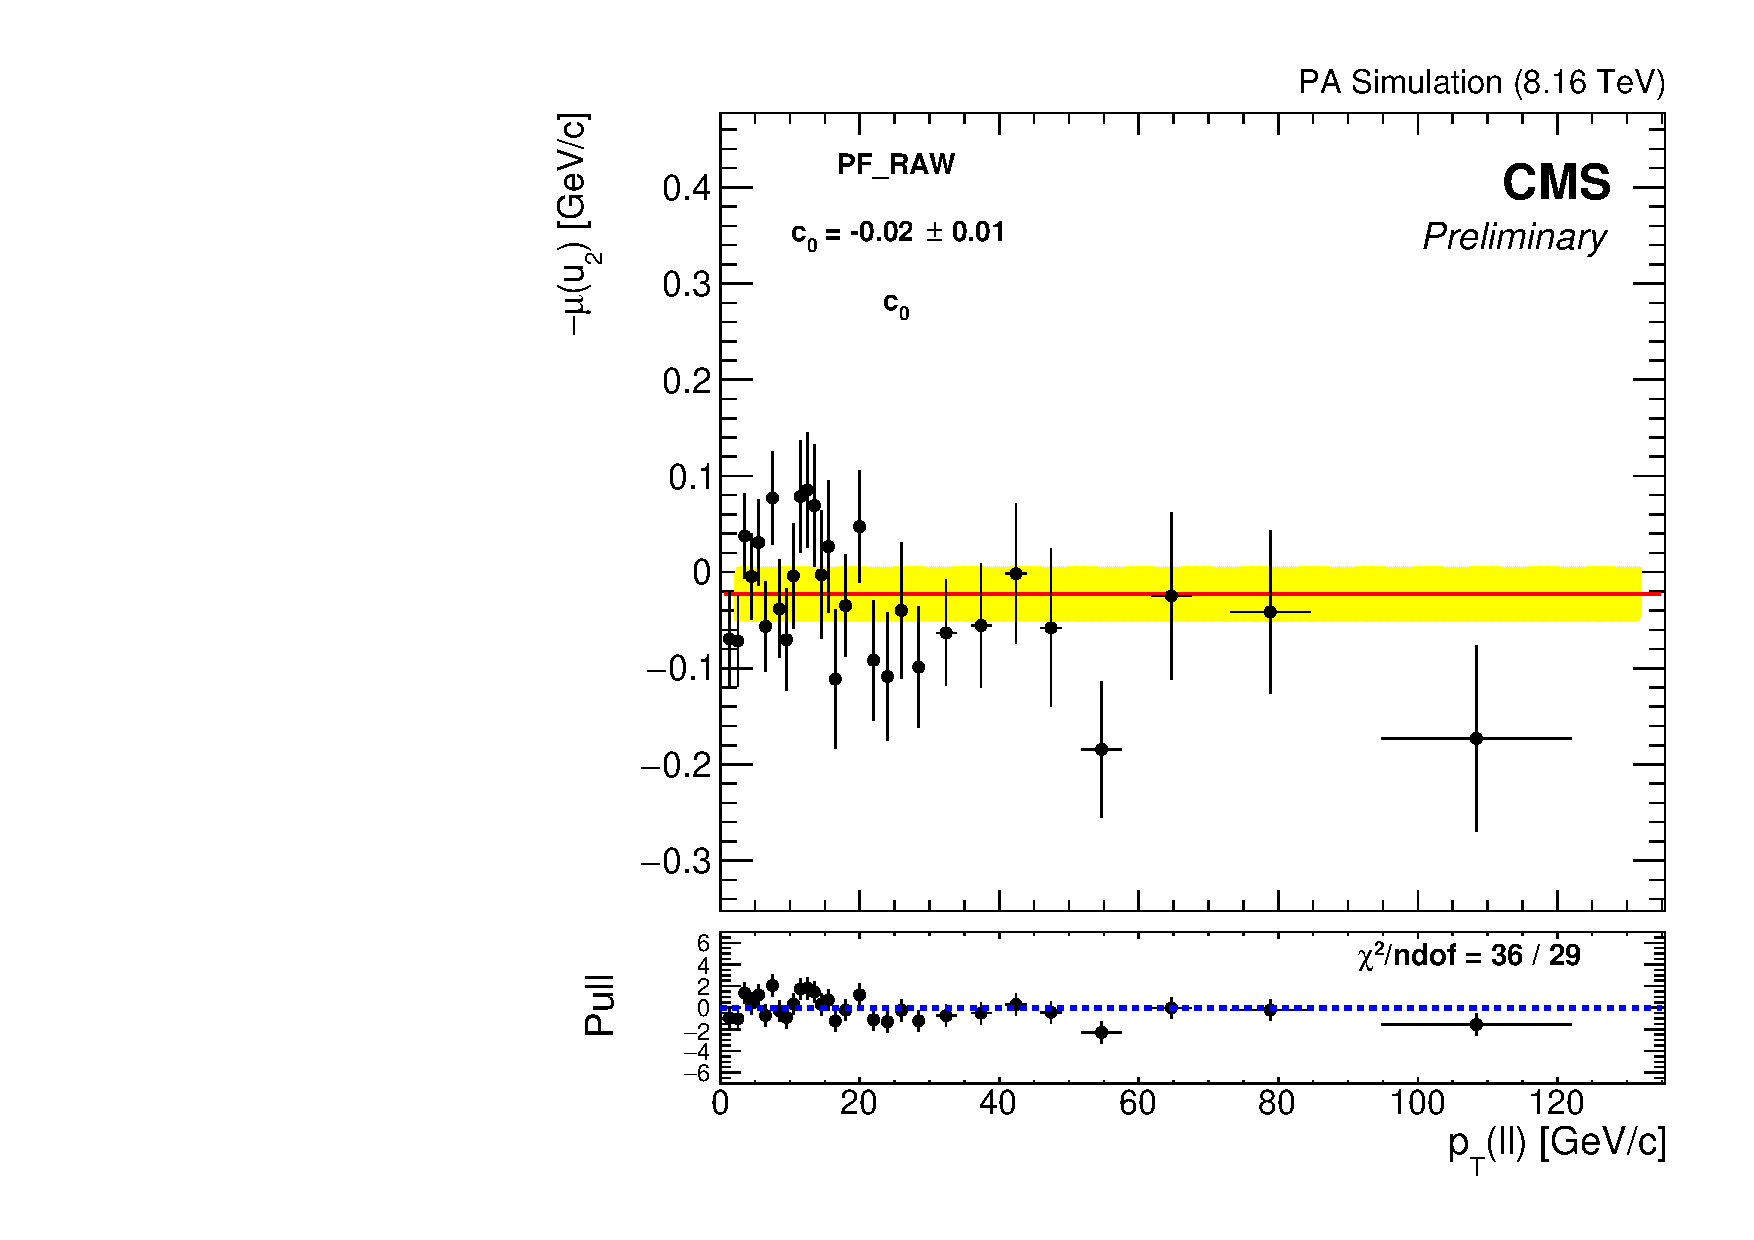
\includegraphics[width=0.4\textwidth]{Figures/WBoson/Analysis/Correction/Recoil/RecoilFitsqT/MC/fitPFu2mean.pdf}
\caption{Fits for the $\mu_{1}$,  $\mu_{2}$ (top) and $\mu$ (bottom) values of perpendicular component of the recoil versus $q_{T}$ for the MC Z boson dimuon sample.}
\label{fig:figU2RecoilScaleFit_MC}
\end{center}
\end{figure}

\clearpage

\subsubsection{Recoil resolution}\label{sec:WBoson_Analysis_Rres}

The resolution parameters $\sigma_{1}$ and  $\sigma_{2}$ for the parallel and perpendicular components of the recoil, obtained from the fits shown in Figures \ref{fig:RecoilFitsData} and \ref{fig:RecoilFitsMC}, are parametrised as a function of $q_{T}$ using the following expression:

\begin{equation}\label{eq:equreolnparam} 
\sigma_{1,2}(q_{T}) = \sqrt{s_{0}^{2} + s_{1}^{2} \cdot q_{T}^{\alpha}},
\end{equation}

The fits for the resolution of the parallel and perpendicular components of the recoil, $\sigma_{1,2}$, in Z samples are shown in Figures \ref{fig:figU1RecoilResolutionFit_data}  and \ref{fig:figU2RecoilResolutionFit_data} for data, and Figures \ref{fig:figU1RecoilResolutionFit_MC} and \ref{fig:figU2RecoilResolutionFit_MC} for MC. In addition, the weighted averages of $\sigma_{1}$ and  $\sigma_{2}$, $\sigma = f \cdot \sigma_{1} + (1 - f) \cdot \sigma_{2}$, are also shown.

\begin{figure} [h!]
\begin{center}
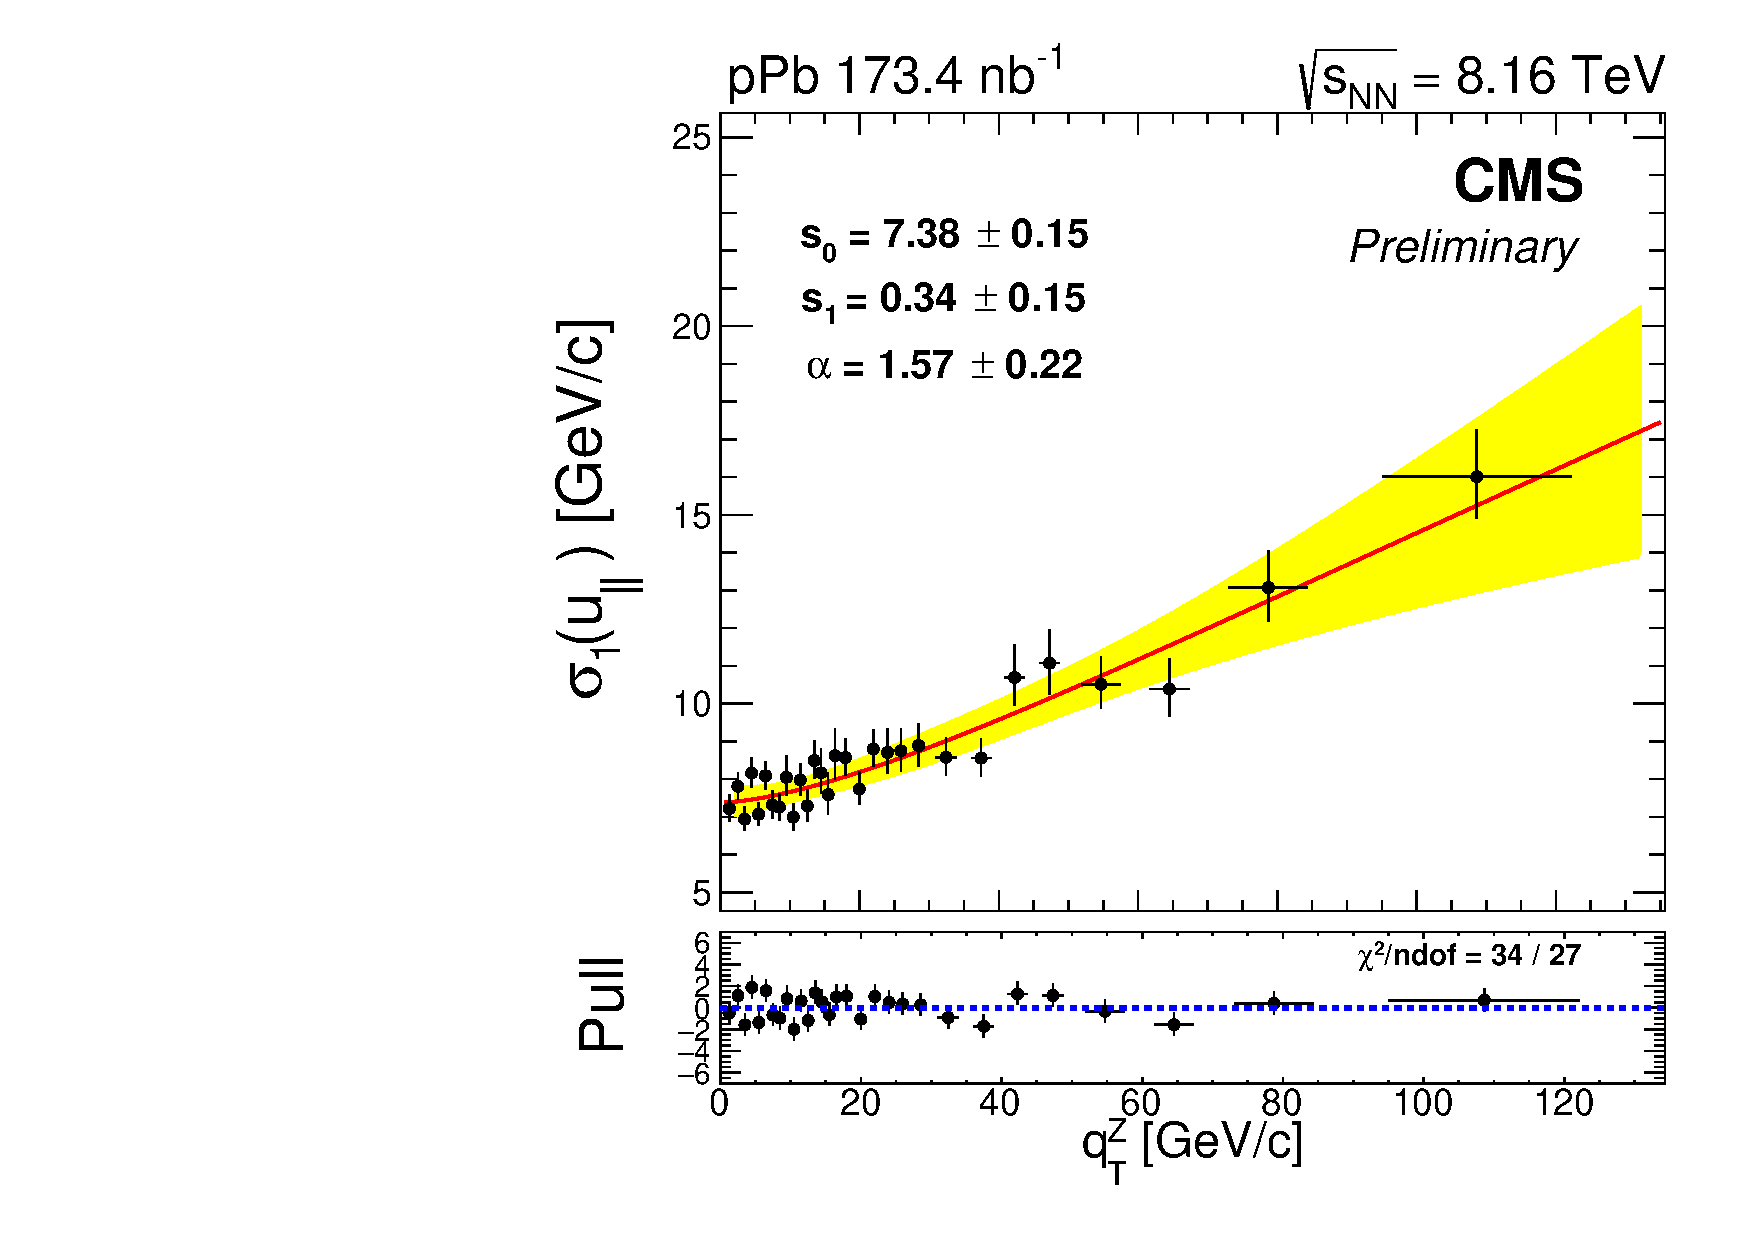
\includegraphics[width=0.4\textwidth]{Figures/WBoson/Analysis/Correction/Recoil/RecoilFitsqT/Data/fitPFu1sigma1.pdf}
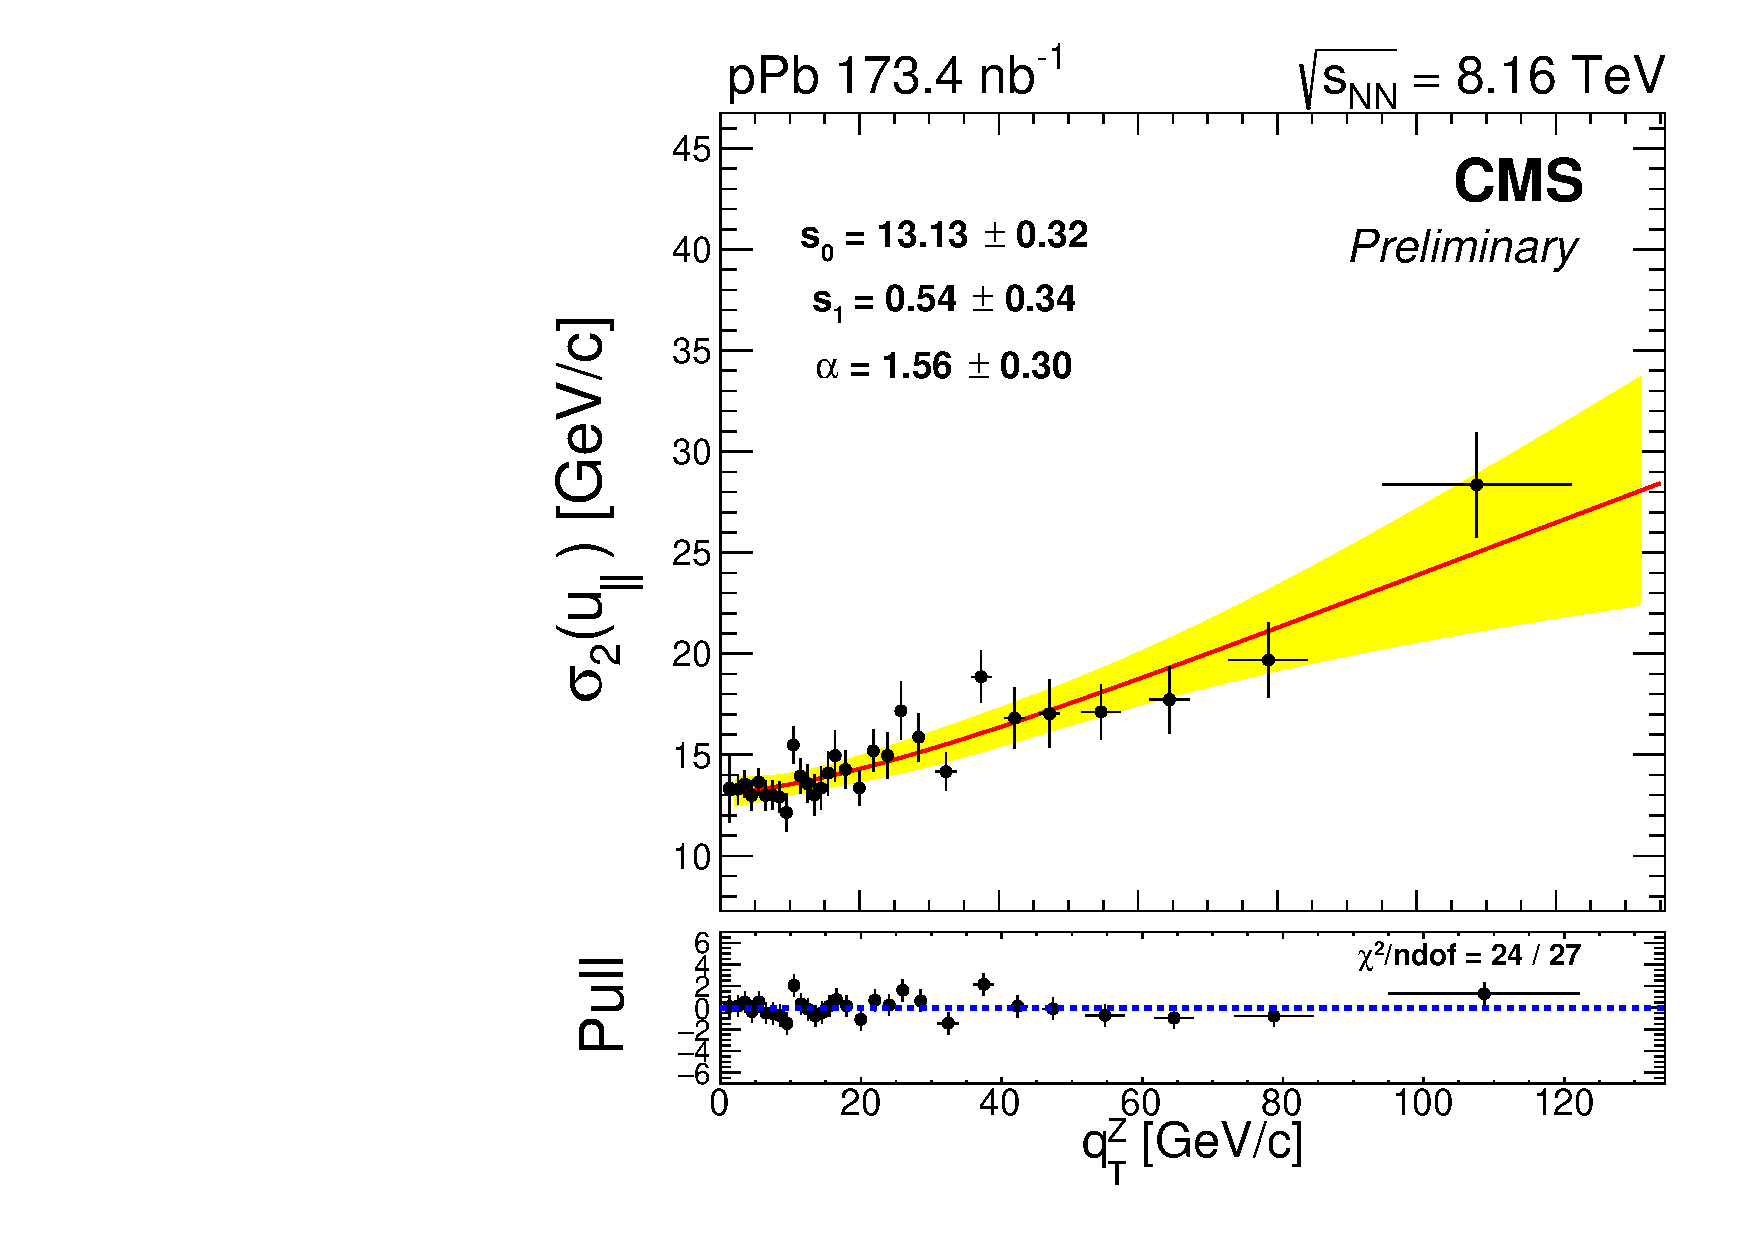
\includegraphics[width=0.4\textwidth]{Figures/WBoson/Analysis/Correction/Recoil/RecoilFitsqT/Data/fitPFu1sigma2.pdf} \\
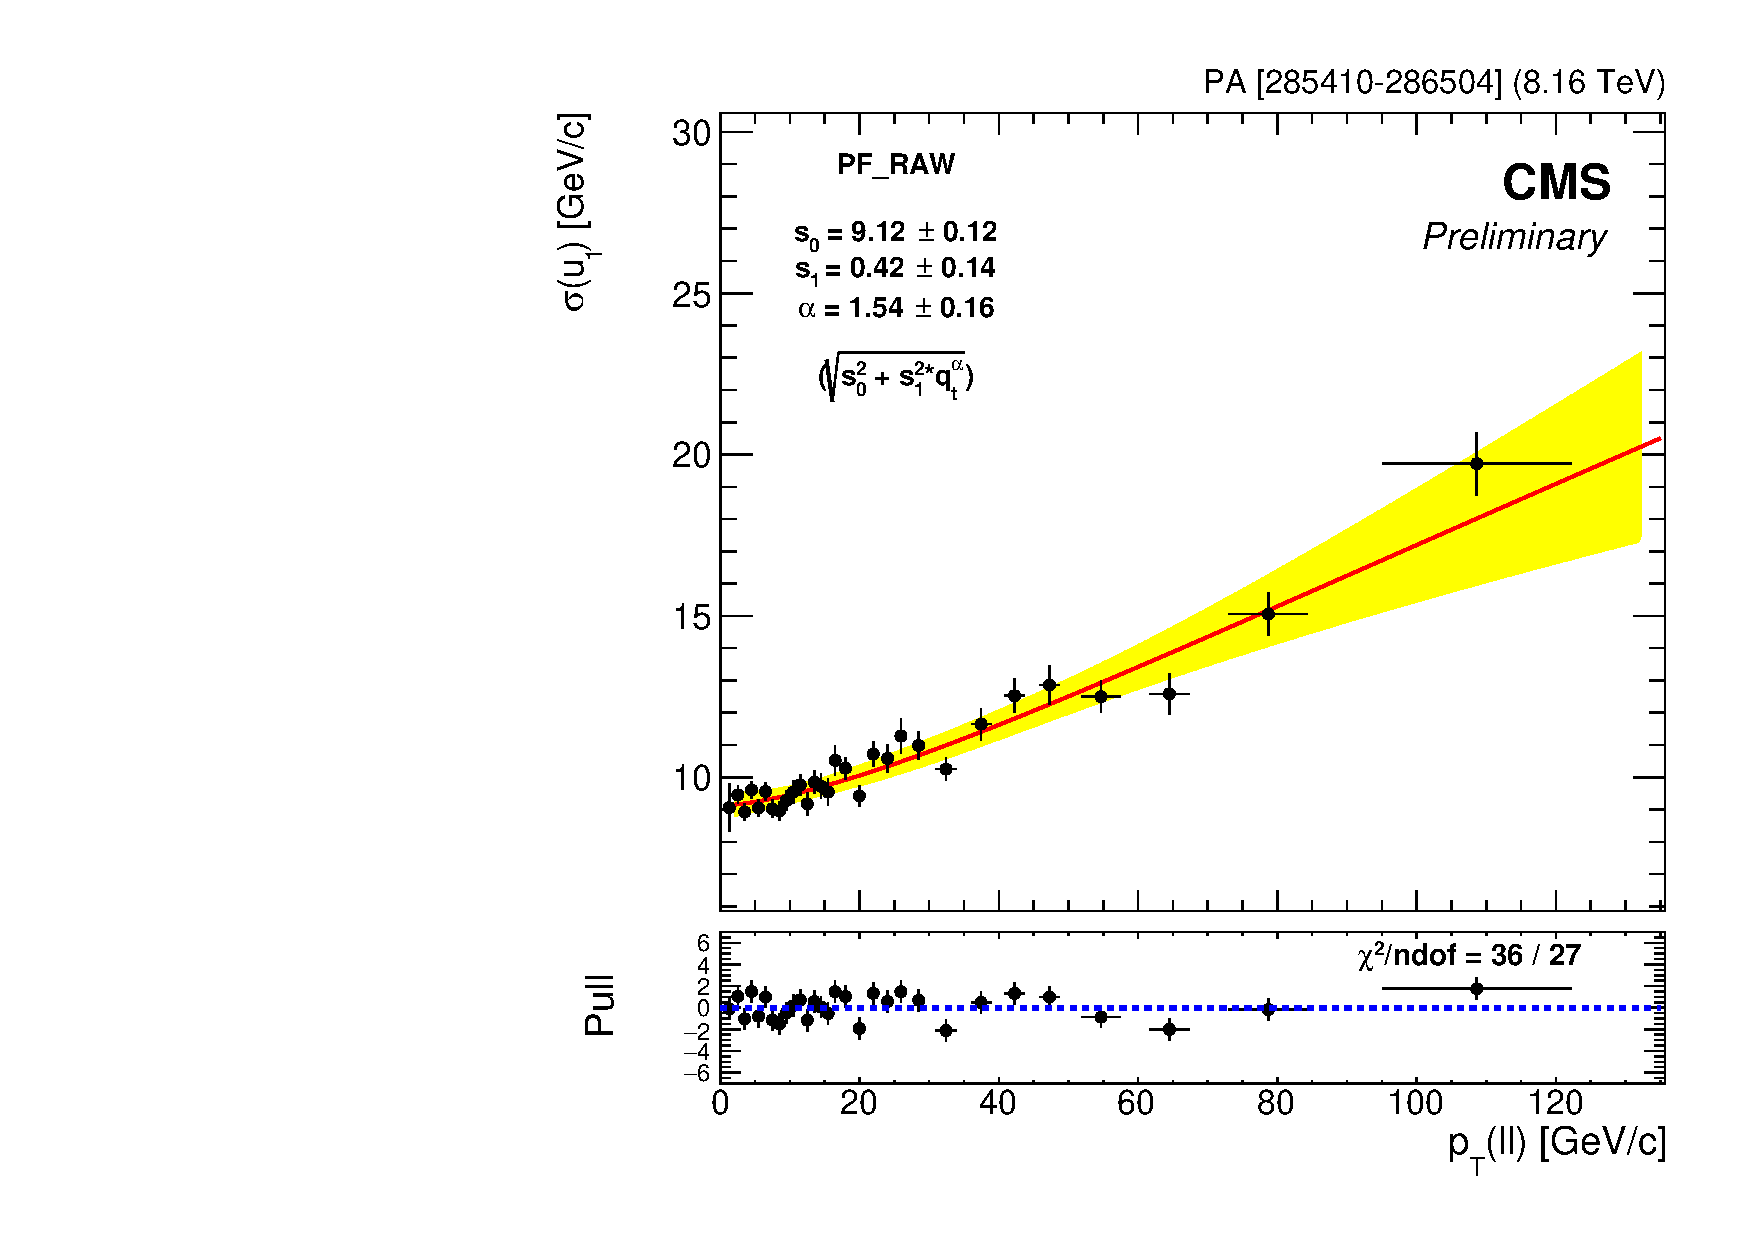
\includegraphics[width=0.4\textwidth]{Figures/WBoson/Analysis/Correction/Recoil/RecoilFitsqT/Data/fitPFu1sigma.pdf}
\caption{Fits for the $\sigma_{1}$,  $\sigma_{2}$ (top) and $\sigma$ (bottom) values of the parallel component of the recoil versus $q_{T}$ for the data Z boson dimuon sample.}
\label{fig:figU1RecoilResolutionFit_data}
\end{center}
\end{figure}

\begin{figure} [h!]
\begin{center}
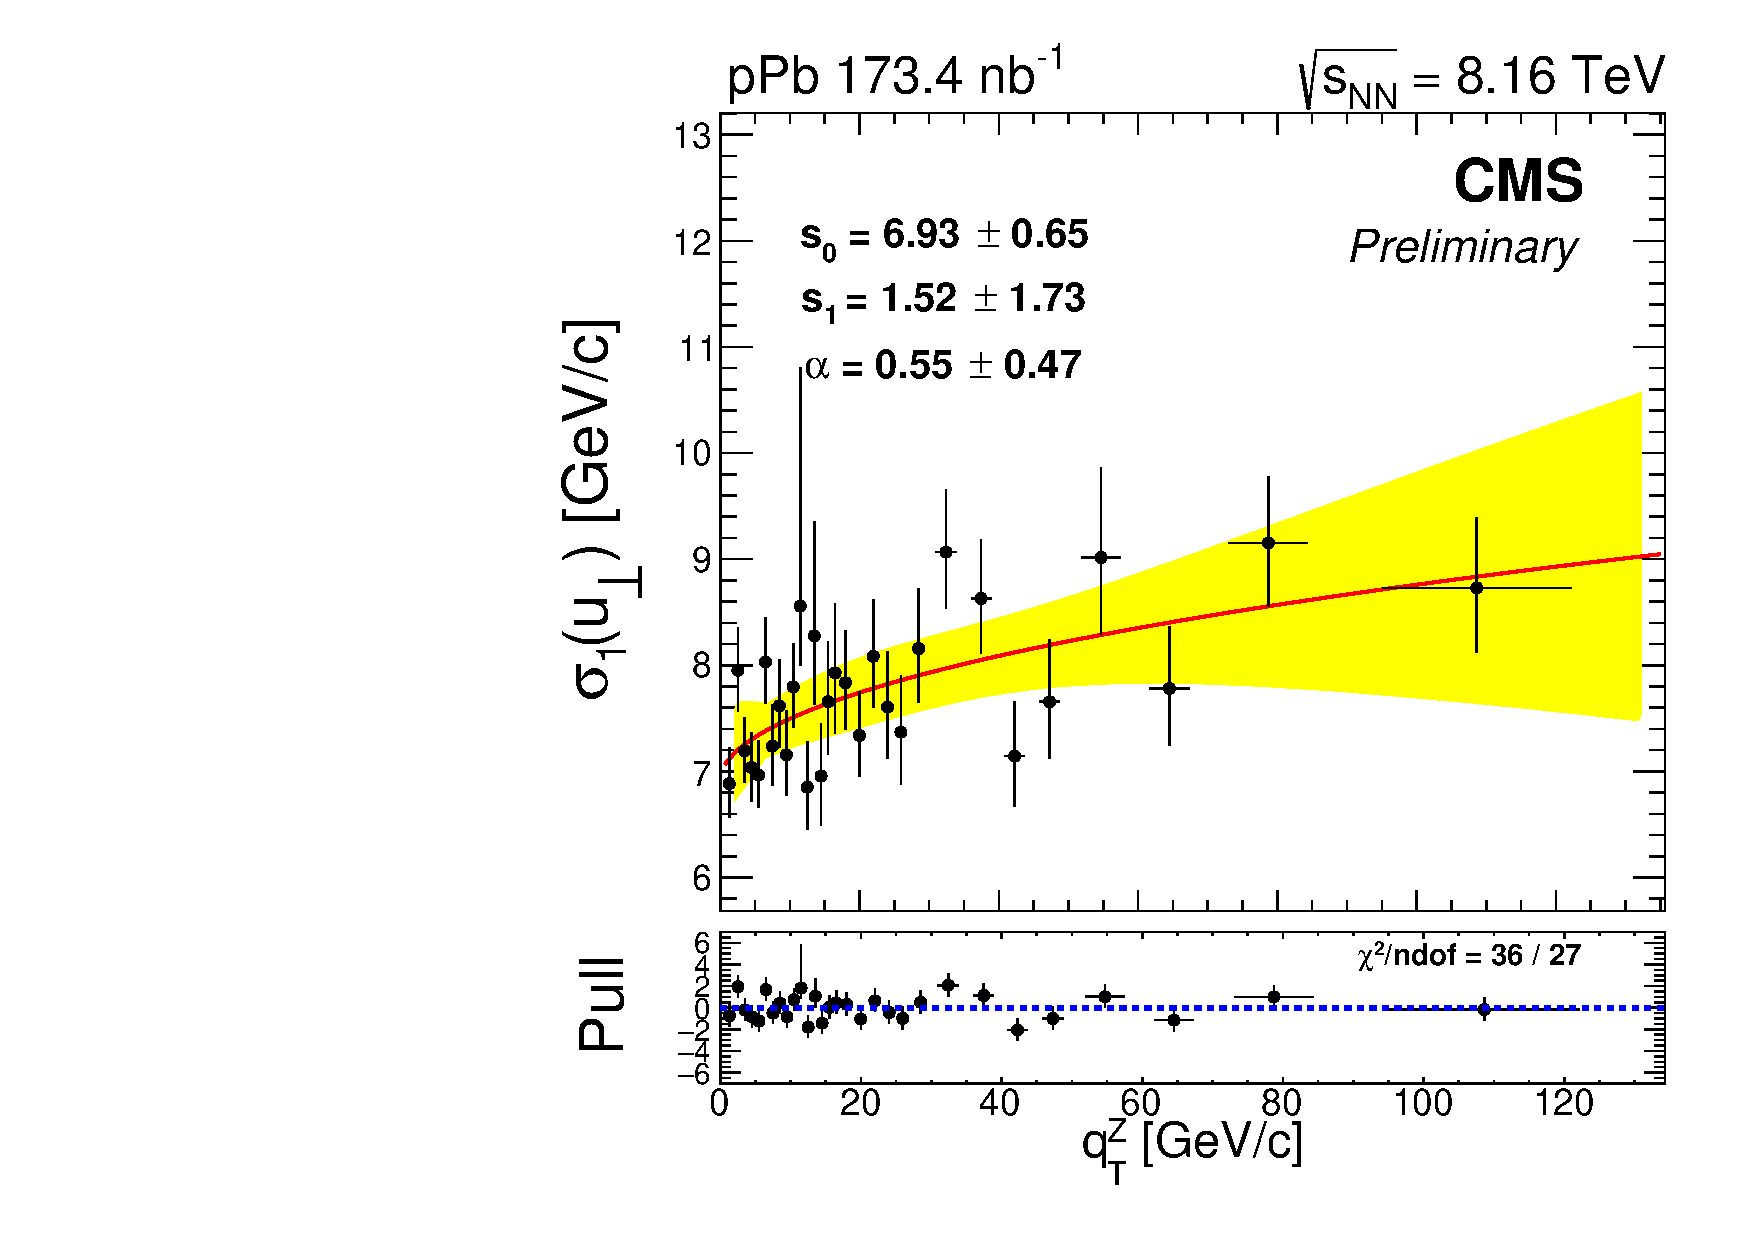
\includegraphics[width=0.4\textwidth]{Figures/WBoson/Analysis/Correction/Recoil/RecoilFitsqT/Data/fitPFu2sigma1.pdf}
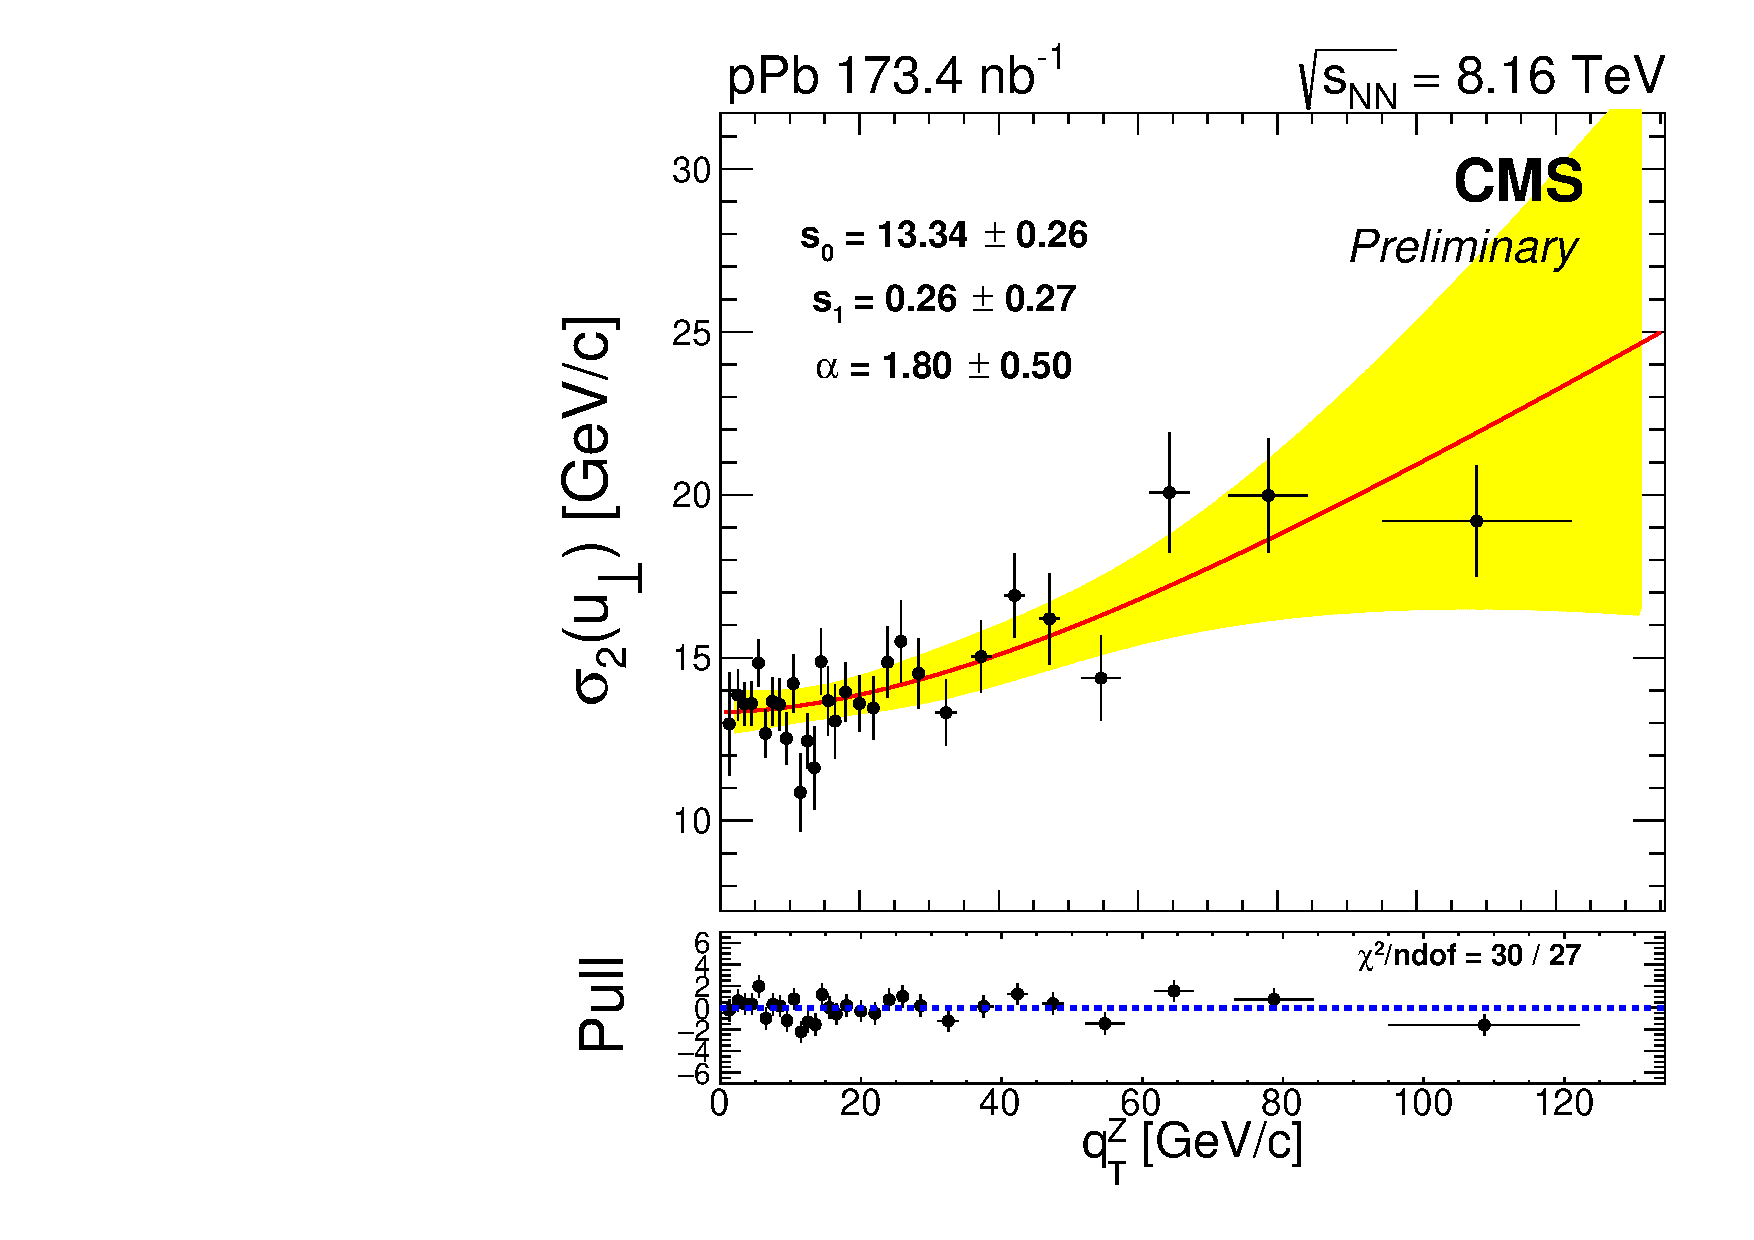
\includegraphics[width=0.4\textwidth]{Figures/WBoson/Analysis/Correction/Recoil/RecoilFitsqT/Data/fitPFu2sigma2.pdf} \\
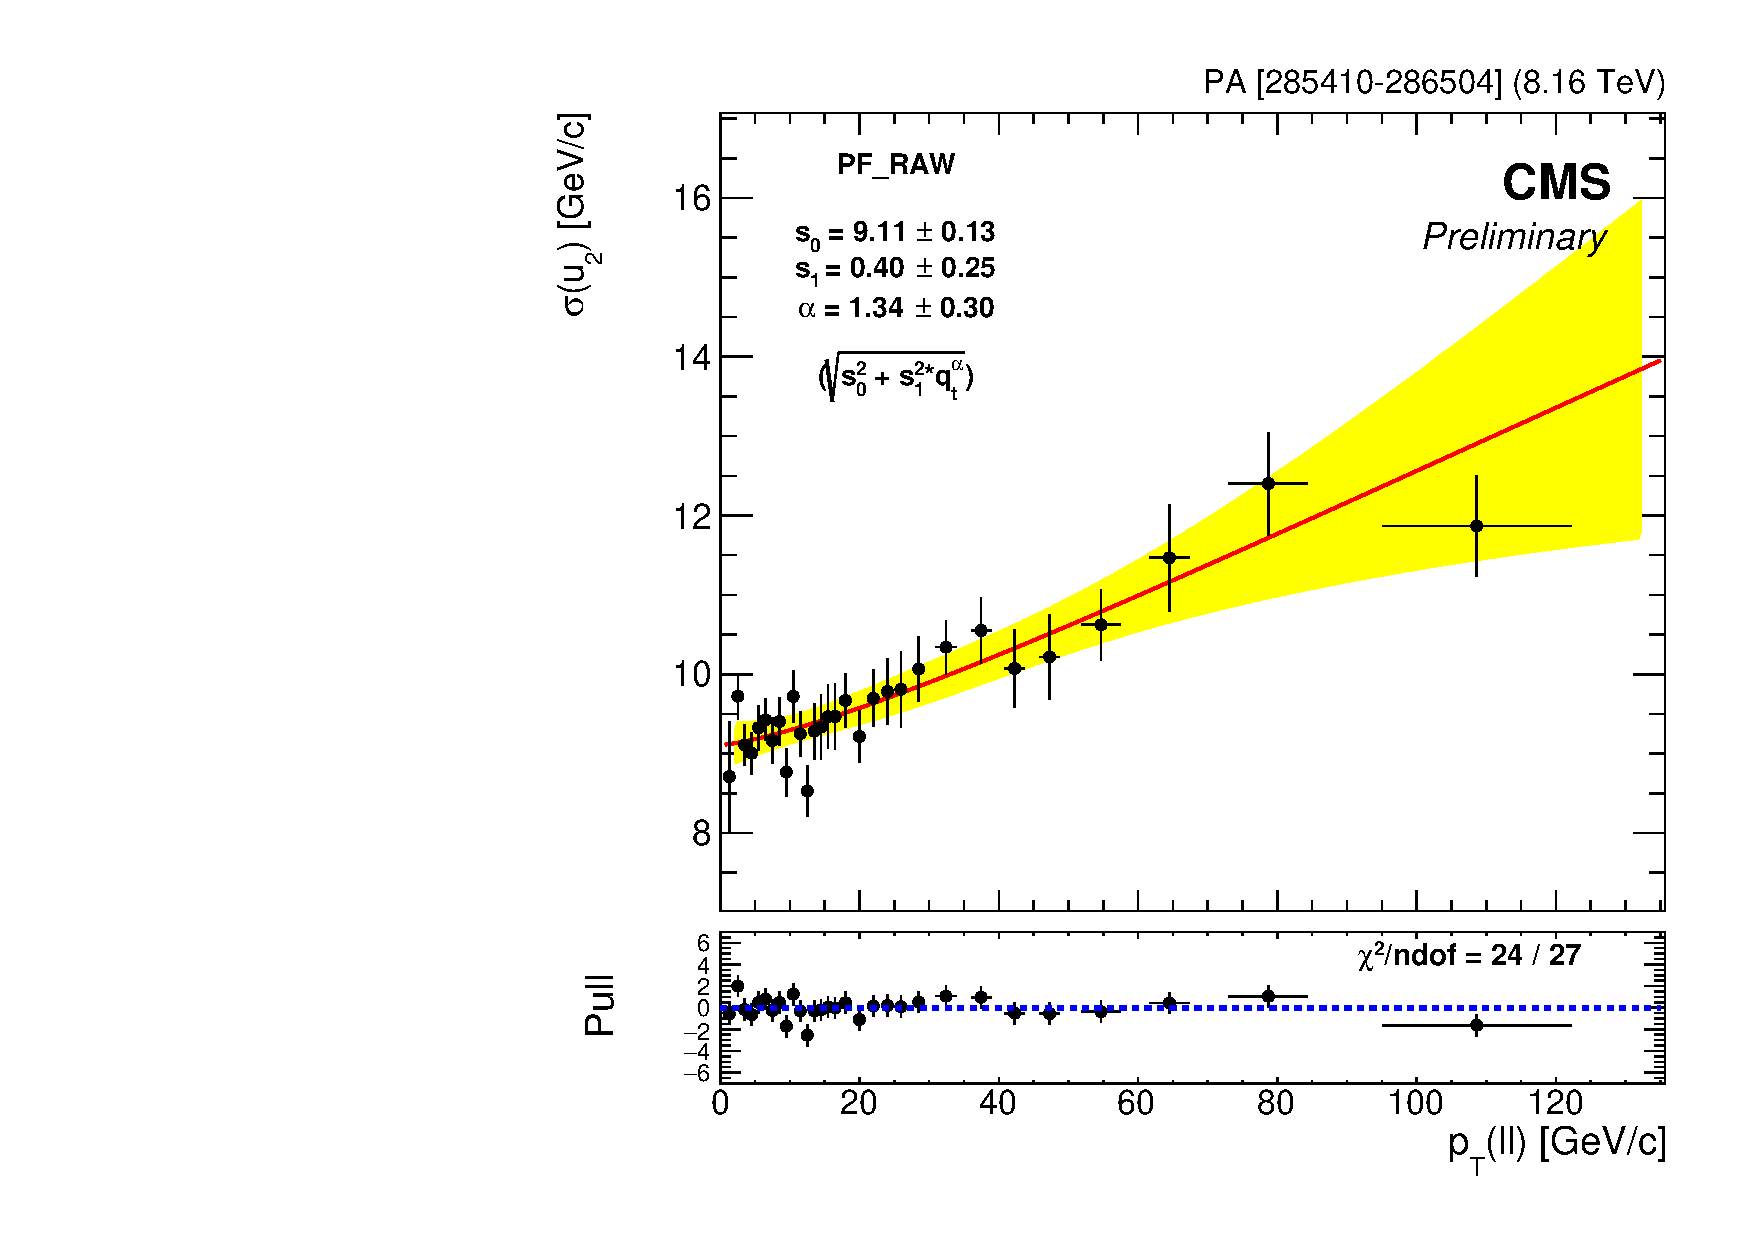
\includegraphics[width=0.4\textwidth]{Figures/WBoson/Analysis/Correction/Recoil/RecoilFitsqT/Data/fitPFu2sigma.pdf}
\caption{Fits for the $\sigma_{1}$,  $\sigma_{2}$ (top) and $\sigma$ (bottom) values of the perpendicular component of the recoil versus $q_{T}$ for the data Z boson dimuon sample.}
\label{fig:figU2RecoilResolutionFit_data}
\end{center}
\end{figure}

\begin{figure} [h!]
\begin{center}
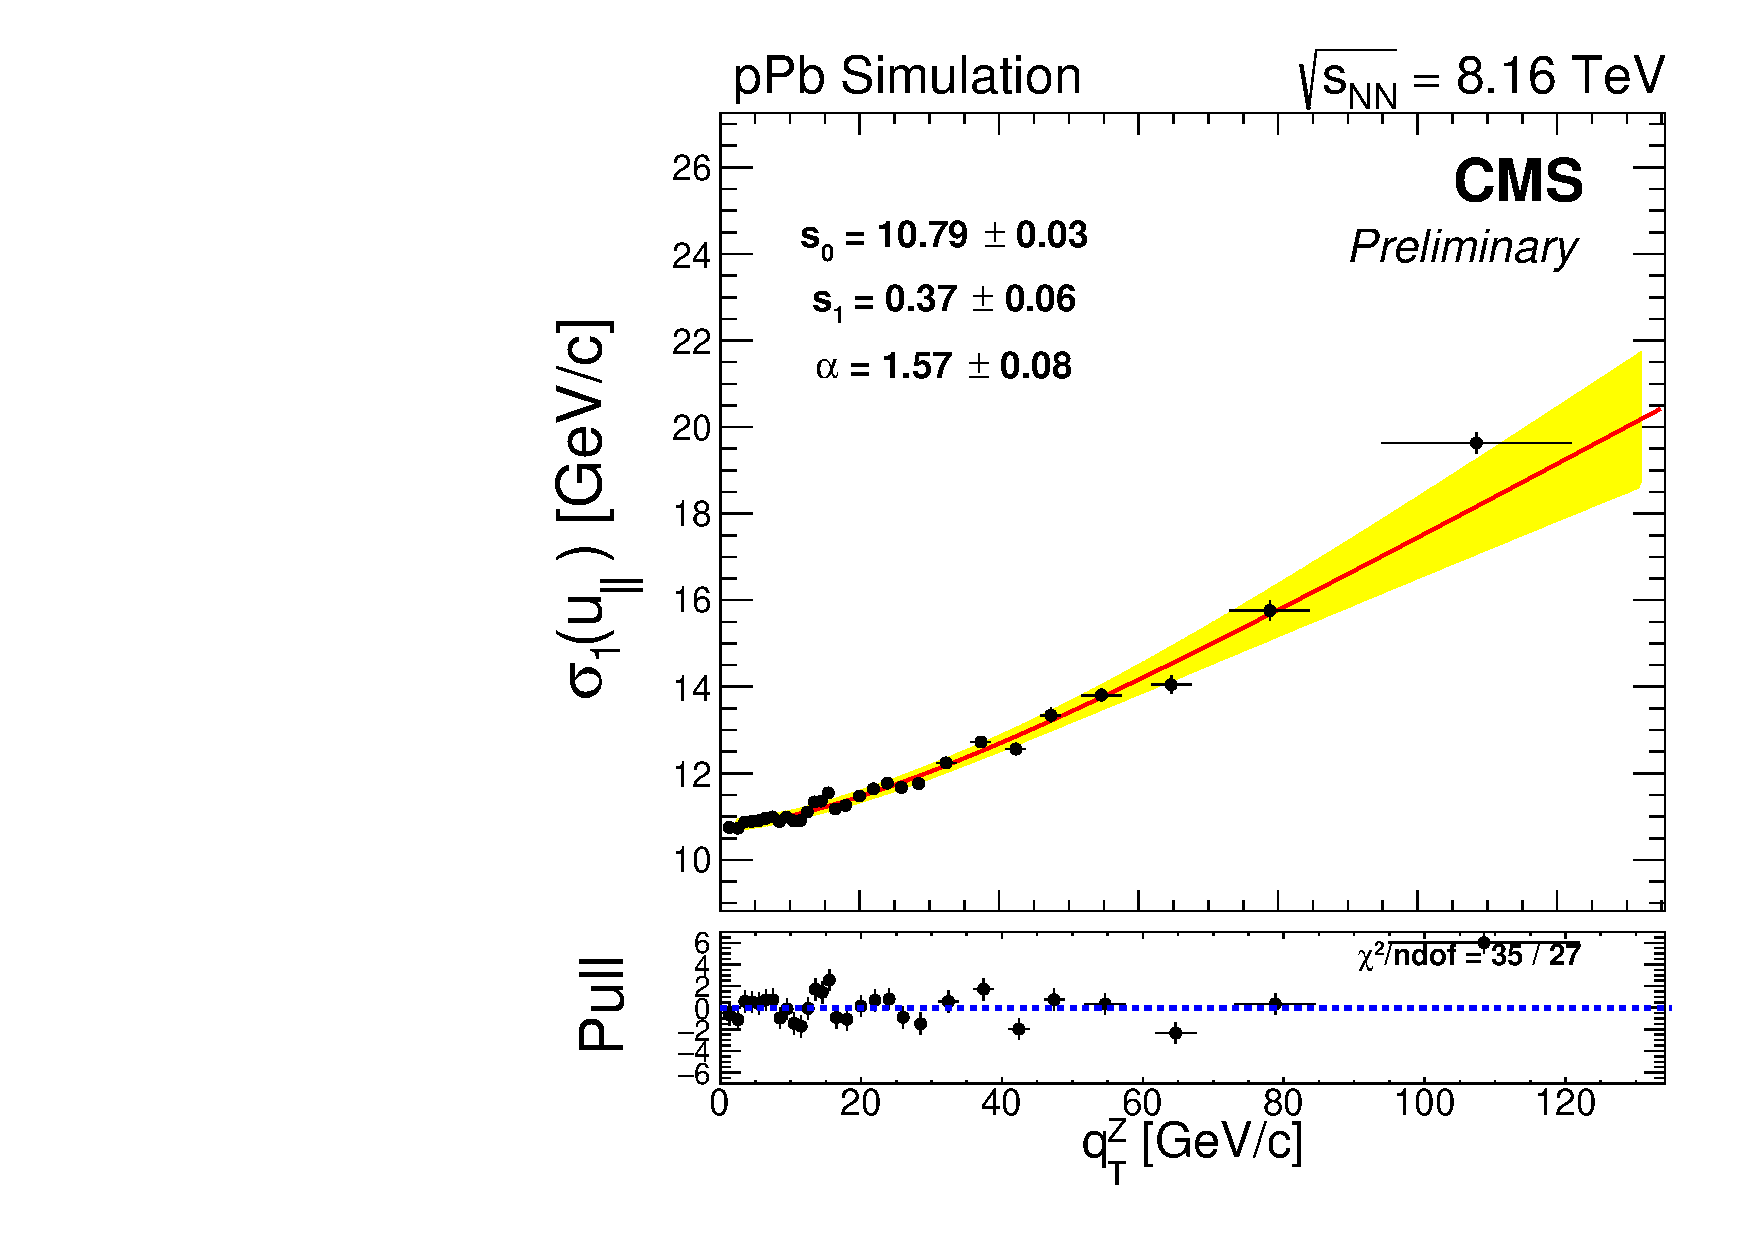
\includegraphics[width=0.4\textwidth]{Figures/WBoson/Analysis/Correction/Recoil/RecoilFitsqT/MC/fitPFu1sigma1.pdf}
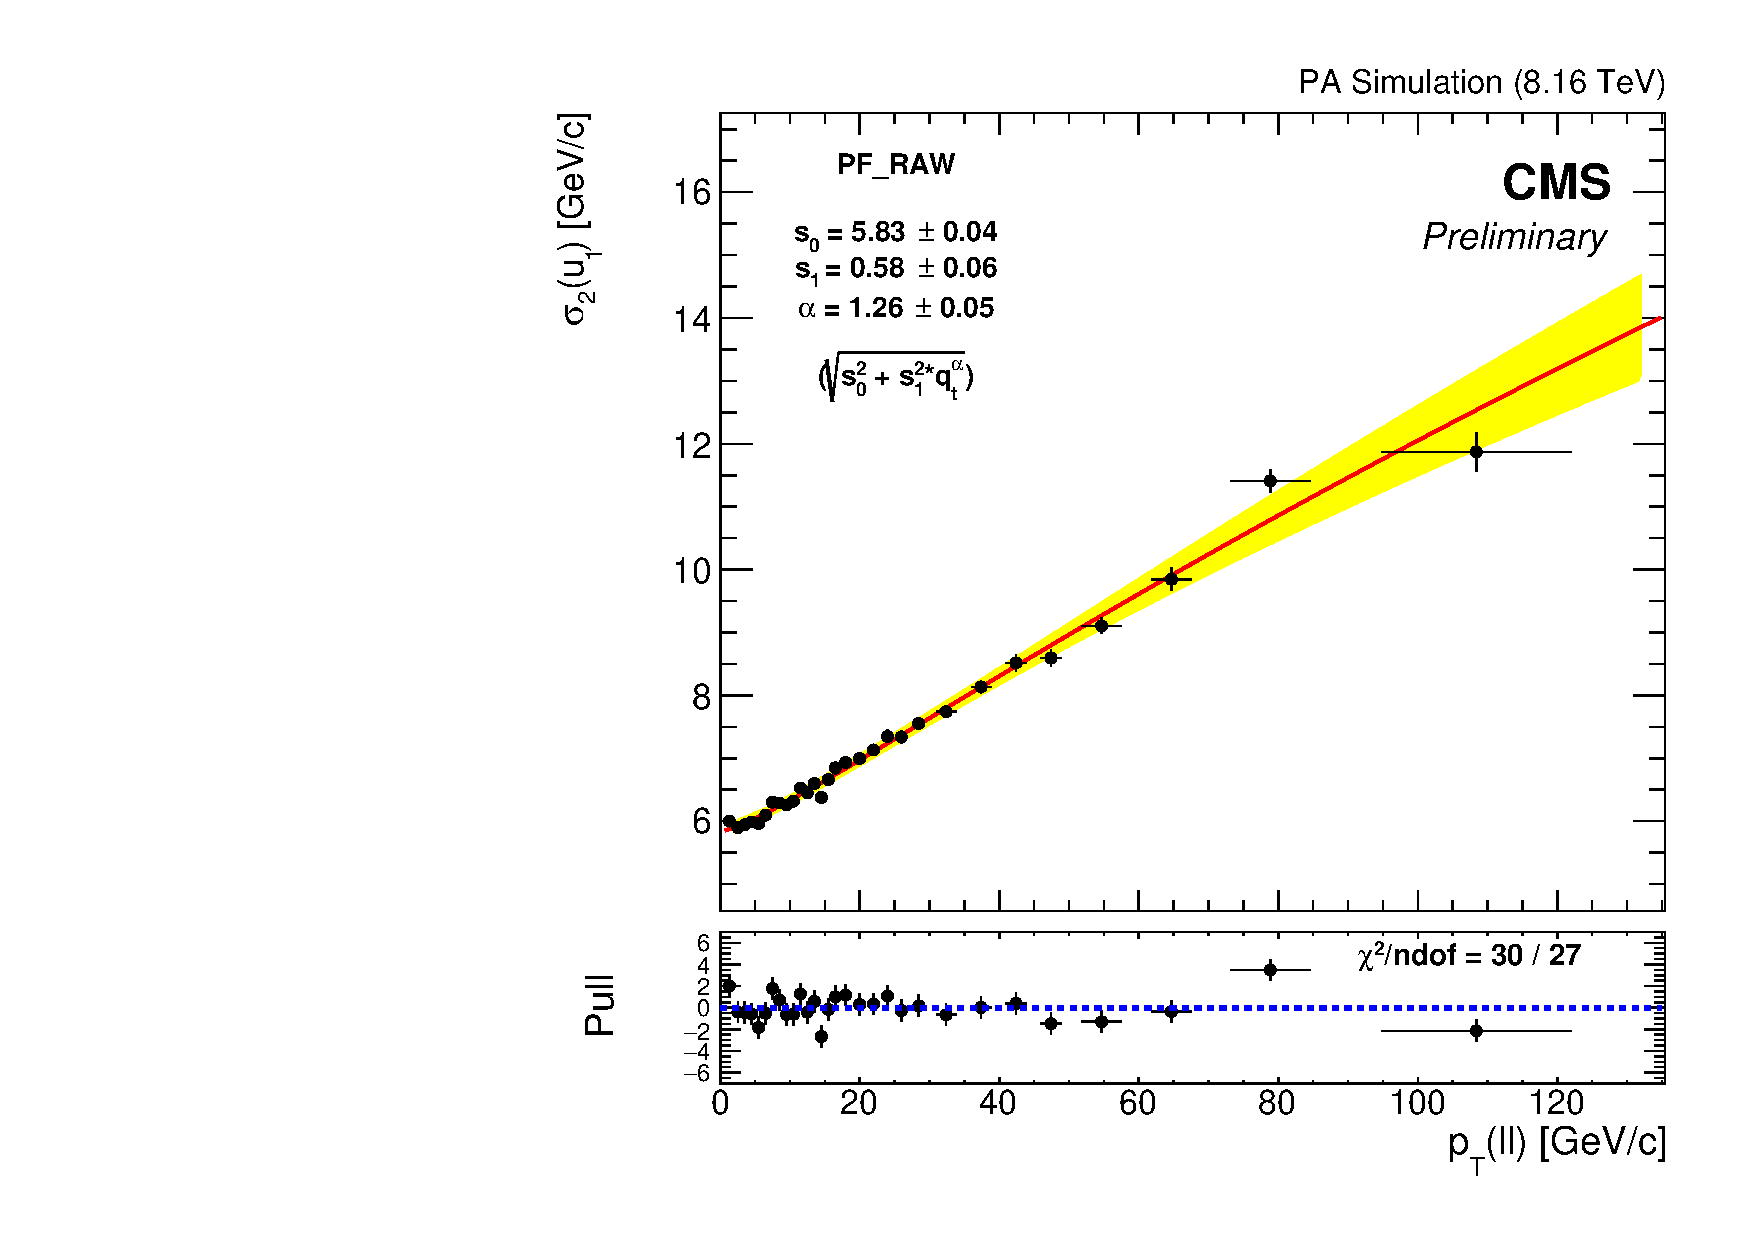
\includegraphics[width=0.4\textwidth]{Figures/WBoson/Analysis/Correction/Recoil/RecoilFitsqT/MC/fitPFu1sigma2.pdf} \\
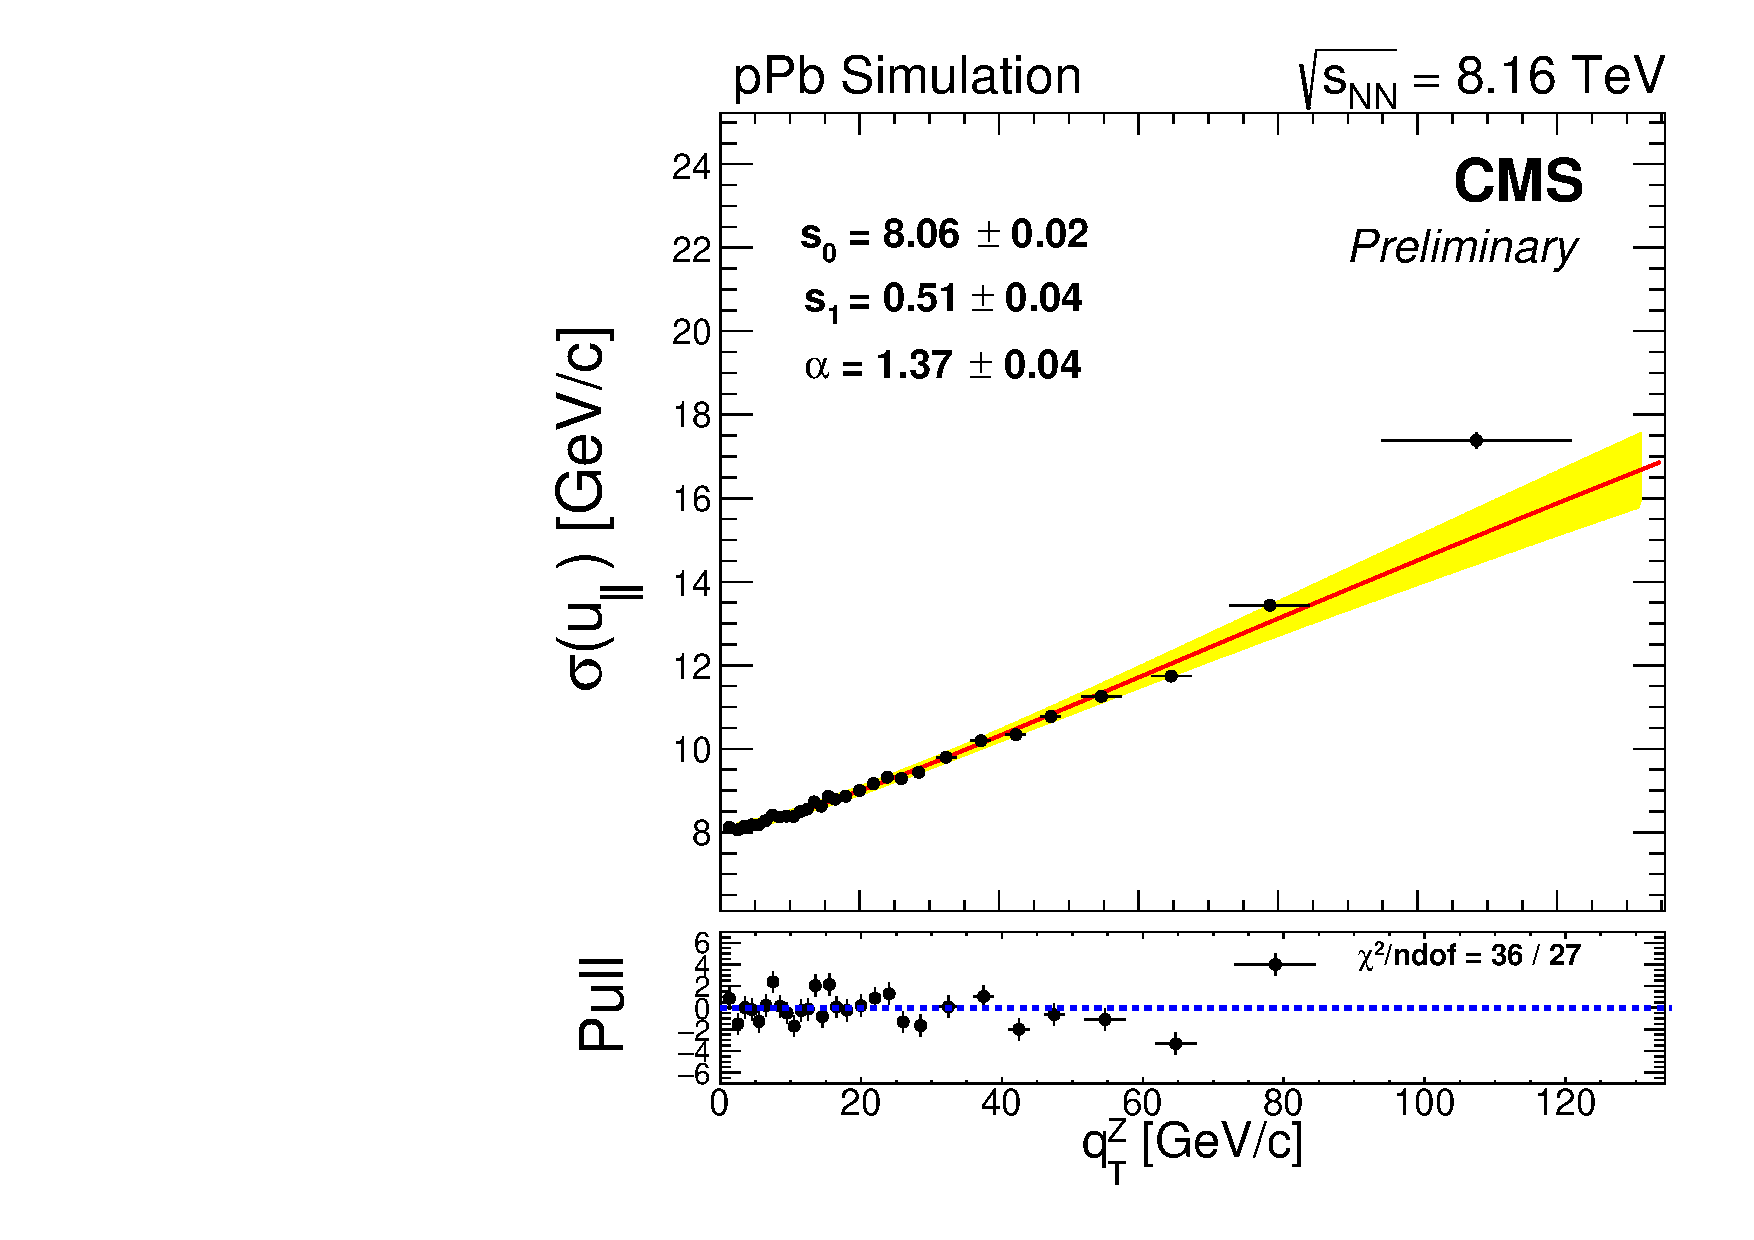
\includegraphics[width=0.4\textwidth]{Figures/WBoson/Analysis/Correction/Recoil/RecoilFitsqT/MC/fitPFu1sigma.pdf}
\caption{Fits for the $\sigma_{1}$,  $\sigma_{2}$ (top) and $\sigma$ (bottom) values of the parallel component of the recoil versus $q_{T}$ for the MC Z boson dimuon sample.}
\label{fig:figU1RecoilResolutionFit_MC}
\end{center}
\end{figure}

\begin{figure}[h!]
\begin{center}
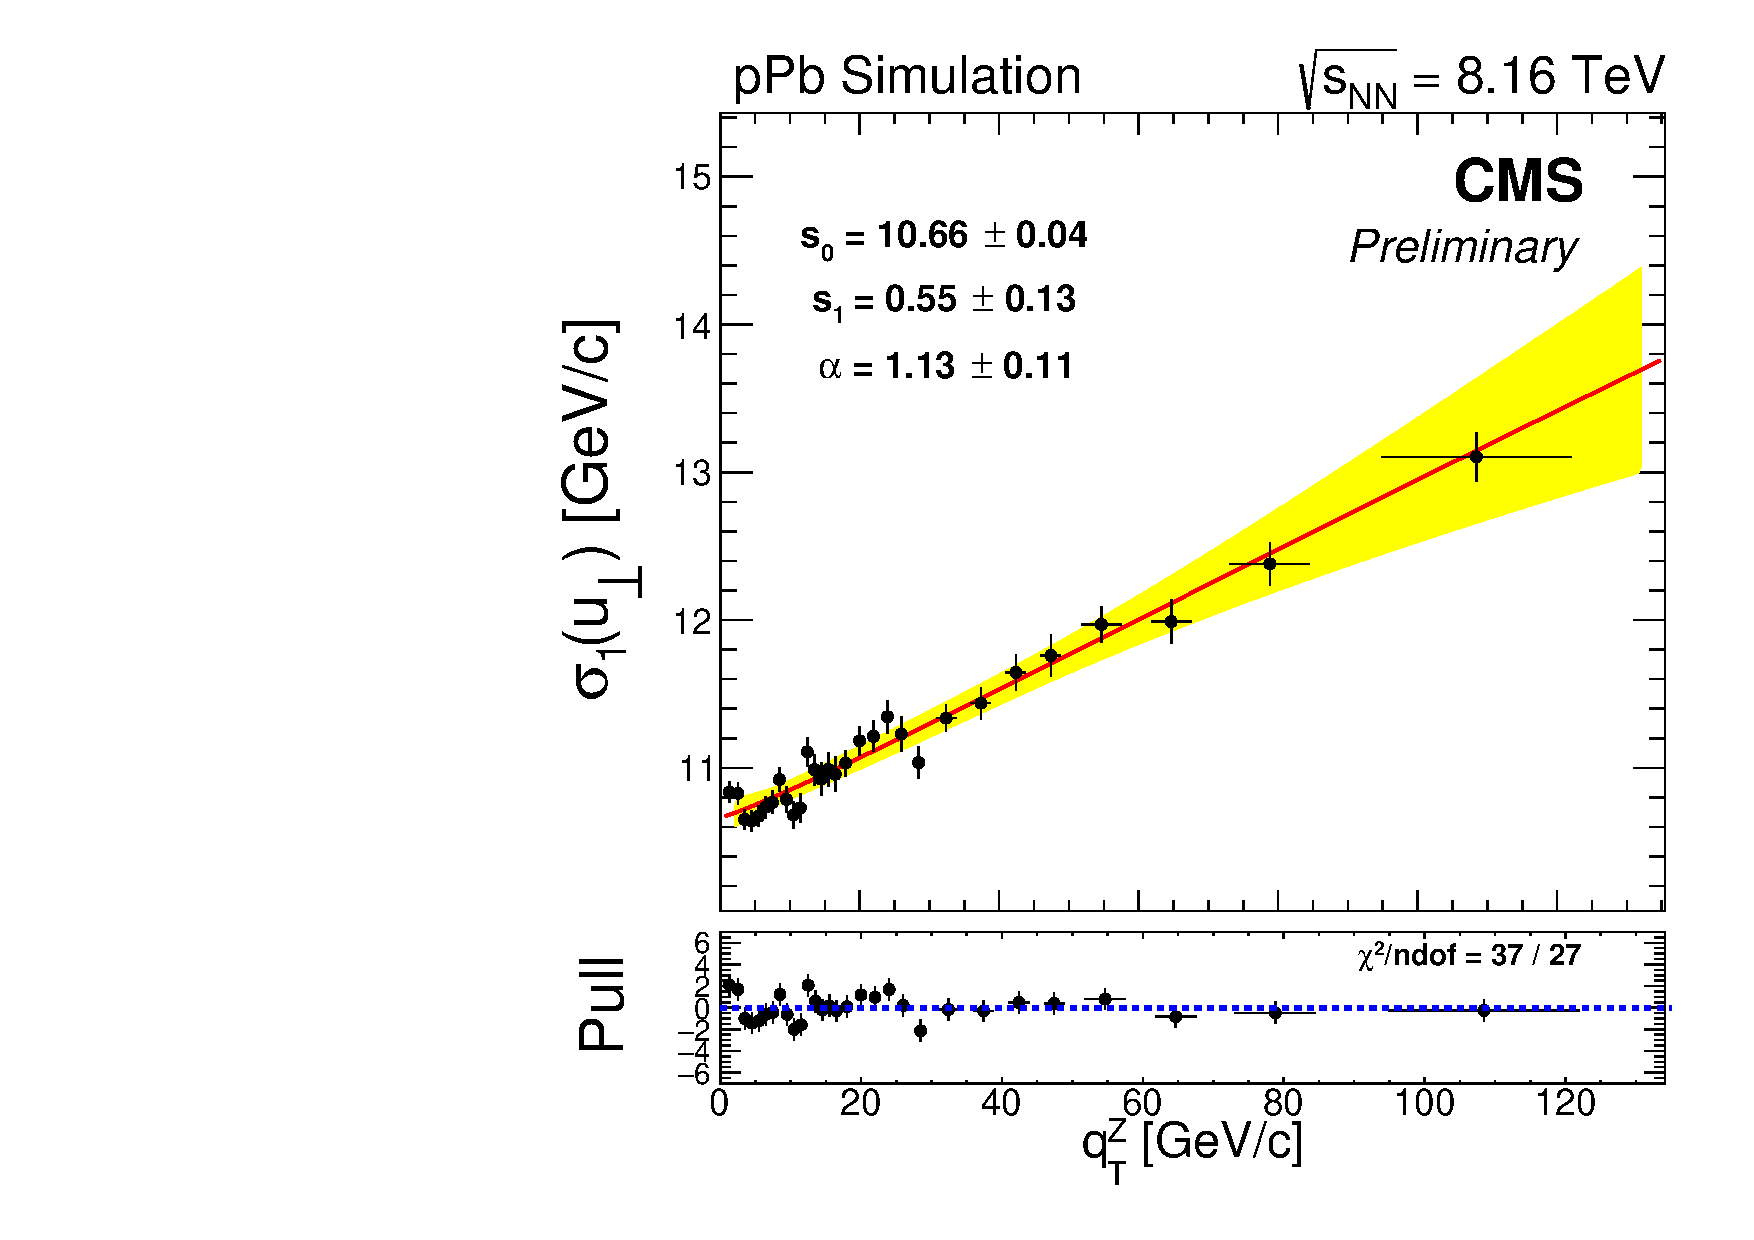
\includegraphics[width=0.4\textwidth]{Figures/WBoson/Analysis/Correction/Recoil/RecoilFitsqT/MC/fitPFu2sigma1.pdf}
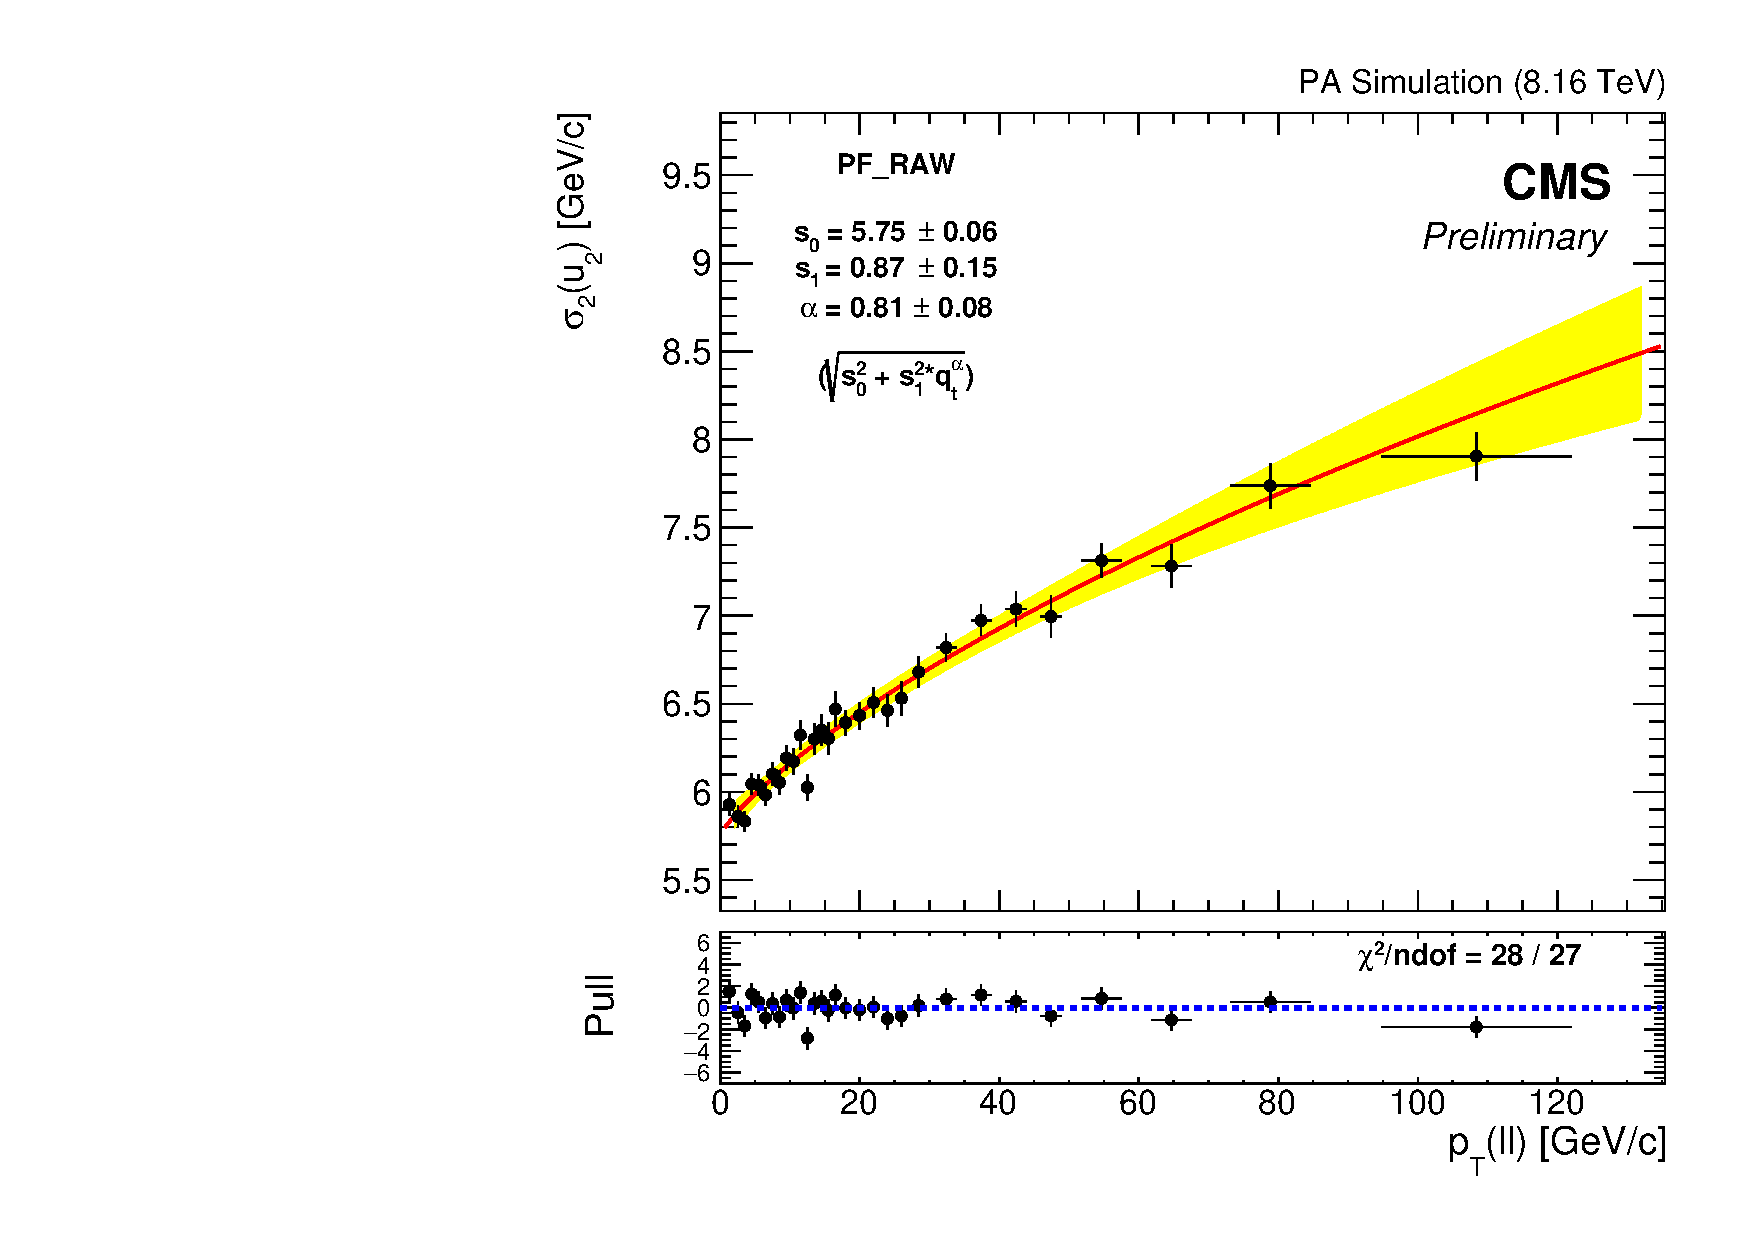
\includegraphics[width=0.4\textwidth]{Figures/WBoson/Analysis/Correction/Recoil/RecoilFitsqT/MC/fitPFu2sigma2.pdf} \\
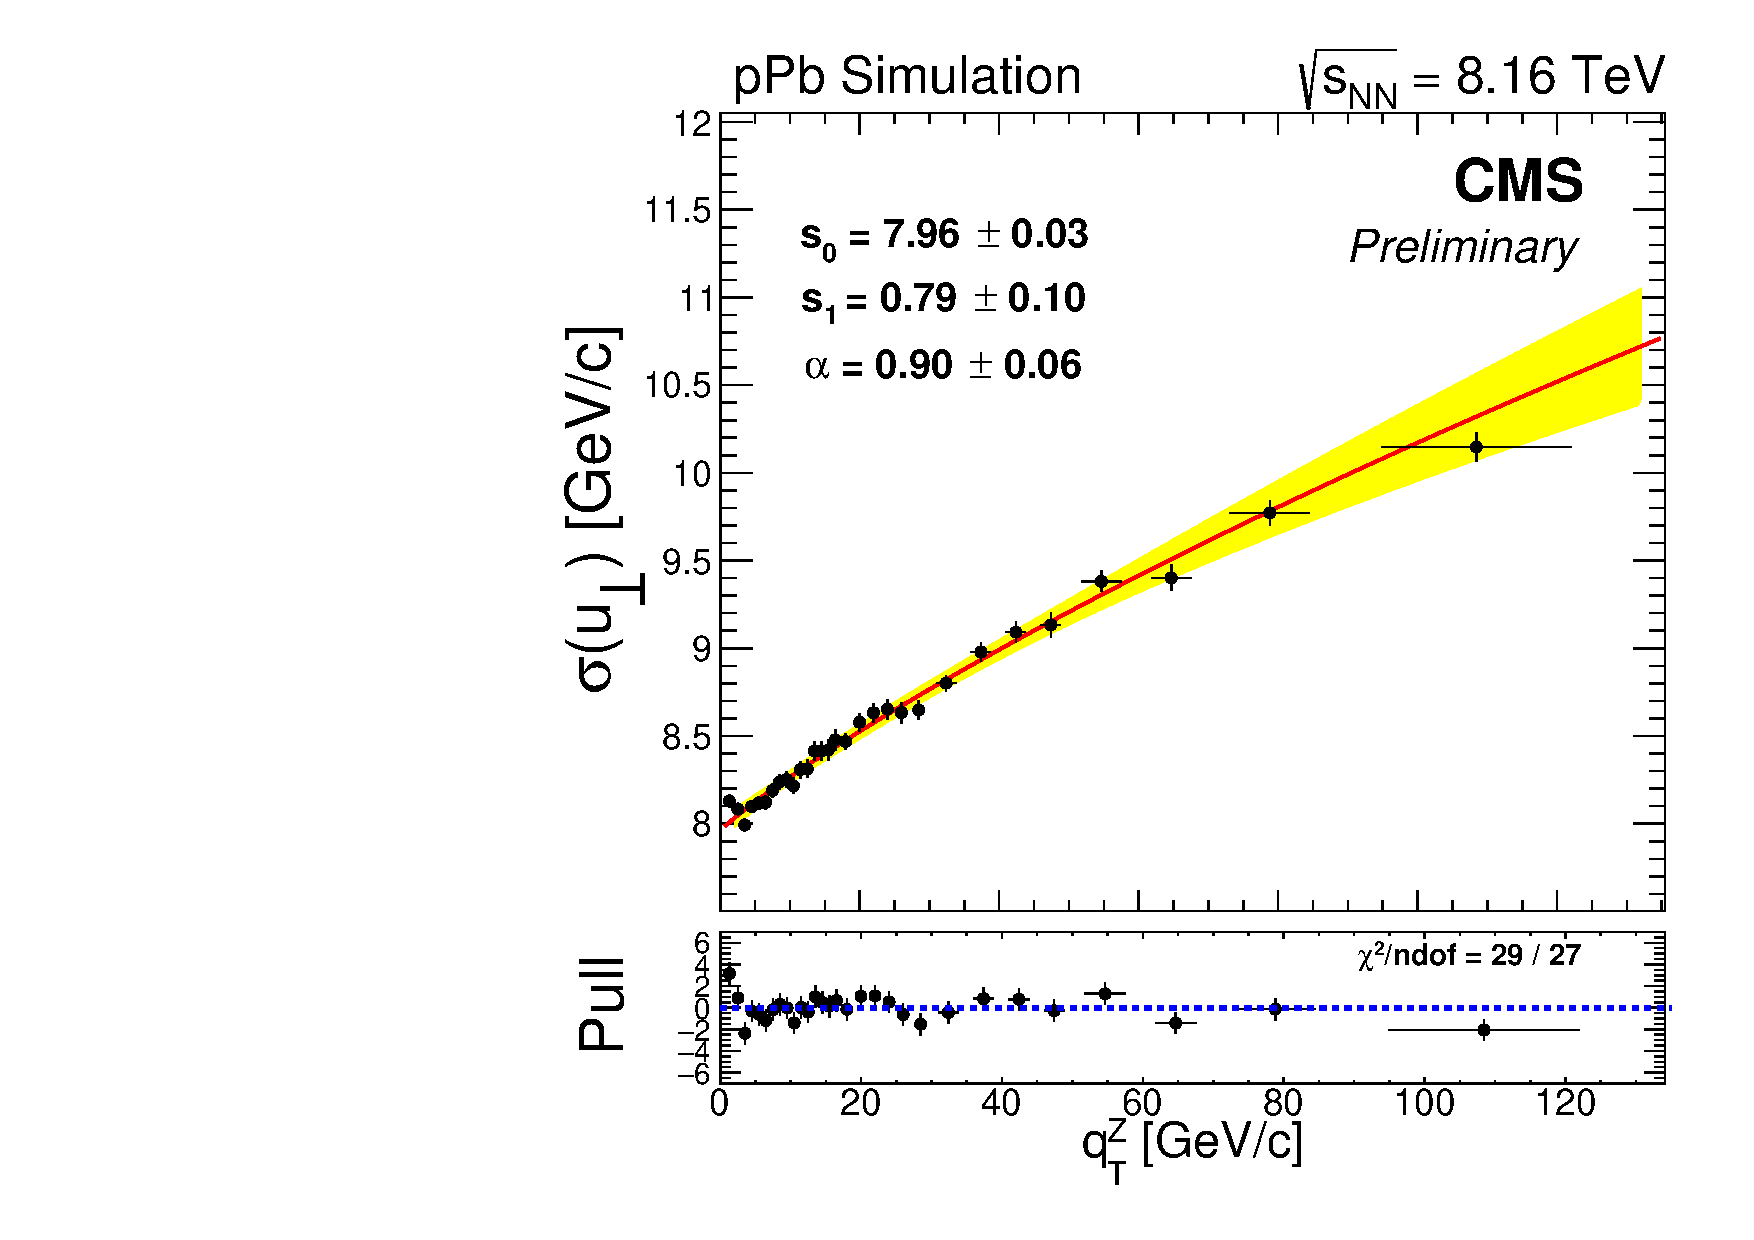
\includegraphics[width=0.4\textwidth]{Figures/WBoson/Analysis/Correction/Recoil/RecoilFitsqT/MC/fitPFu2sigma.pdf}
\caption{Fits for the $\sigma_{1}$,  $\sigma_{2}$ (top) and $\sigma$ (bottom) values of the perpendicular component of the recoil versus $q_{T}$ for the MC Z boson dimuon sample.}
\label{fig:figU2RecoilResolutionFit_MC}
\end{center}
\end{figure}

\clearpage

\subsubsection{Recoil correction}\label{sec:WBoson_Analysis_RecoilCorr}

The recoil corrections are applied to correct the recoil in MC to match the scale and resolution in data. This can be done in two ways:

  \begin{itemize}
  \item Smearing method : in this case, for each event the corrected value of the parallel and perpendicular components of the recoil in MC are obtained from a random sampling of a gaussian function defined as: 
    \begin{equation}\label{eq:eqreccornsmrupar} 
%      u_{\parallel} = Gauss(u_{\parallel} - \tilde{u}_{\parallel}^{MC}(q_{T}) + \tilde{u}_{\parallel}^{data}(q_{T}), \sqrt{{\sigma_{\parallel}^{data}(q_{T},n)}^{2} - {\sigma_{\parallel}^{MC}(q_{T},n)}^{2}})
        u^{corr}_{\parallel} = Gauss(u_{\parallel} - \mu_{\parallel}^{MC}(q_{T}) + \mu_{\parallel}^{data}(q_{T}), \sqrt{{\sigma_{\parallel}^{data}(q_{T})}^{2} - {\sigma_{\parallel}^{MC}(q_{T})}^{2}}) \quad,
    \end{equation}
    \begin{equation}\label{eq:eqreccornsmruperp} 
%      u_{\perp} = Gauss(u_{\perp}, \sqrt{{\sigma_{\perp}^{data}(q_{T},n)}^{2} - {\sigma_{\perp}^{MC}(q_{T},n)}^{2}})
        u^{corr}_{\perp} = Gauss(u_{\perp}, \sqrt{{\sigma_{\perp}^{data}(q_{T})}^{2} - {\sigma_{\perp}^{MC}(q_{T})}^{2}}) \quad,
    \end{equation}
    
    where $\mu$ and $\sigma$ are the weighted average values obtained in the previous section.
    
    \item Scaling method :  in this case we have two different options,
    
      \begin{itemize}
       \item General case: the Cumulative Distribution Function (CDF) of the weighted sum of the two Gaussian functions in \eq{eq:gaussFit} for data and MC are used,
       \begin{equation}\label{eq:eqRecCorrGeneralCase} 
         u^{corr}_{\parallel, \perp} = CDF^{-1}_{data}[CDF_{MC}[u_{\parallel, \perp}^{MC}]]
       \end{equation}
       
       \item Gaussian case: the weighted average values $\mu$ and $\sigma$ obtained in the previous section are used to scale the recoil in MC,
       \begin{equation}\label{eq:eqreccornsclupar} 
         u^{corr}_{\parallel} = (u_{\parallel} - \mu_{\parallel}^{MC}(q_{T}))\frac{\sigma_{\parallel}^{data}(q_{T})}{\sigma_{\parallel}^{MC}(q_{T})} + \mu_{\parallel}^{data}(q_{T}),
       \end{equation}
       \begin{equation}\label{eq:eqreccornscluperp} 
         u^{corr}_{\perp} = u_{\perp}\frac{\mu_{\perp}^{data}(q_{T})}{\sigma_{\perp}^{MC}(q_{T})}
       \end{equation}
      \end{itemize}

  \end{itemize}

Finally the MET in MC is recalculated after correcting the recoil as $\mathrm{MET}_{corr} = \abs{\vec{p}^{\mu}_{T} + \vec{u}_{corr}}$


\subsubsection{Closure tests}\label{sec:WBoson_Analysis_closureTests}

The corrections for MET that are extracted from the control sample (Z boson selected events) are reapplied to the control sample as a check. For this closure test, the scaling recoil correction method in the gaussian case is used. In Figure \ref{fig:recoilClosure} we show the data and MC (including HF reweighting) corrected distributions for PW RAW MET for the full pseudorapidity region (left) and a selected pseudorapidity bin (right). We can see that the agreement between MC after recoil correction and data is now pretty good.


\begin{figure}[!h]
\begin{center}
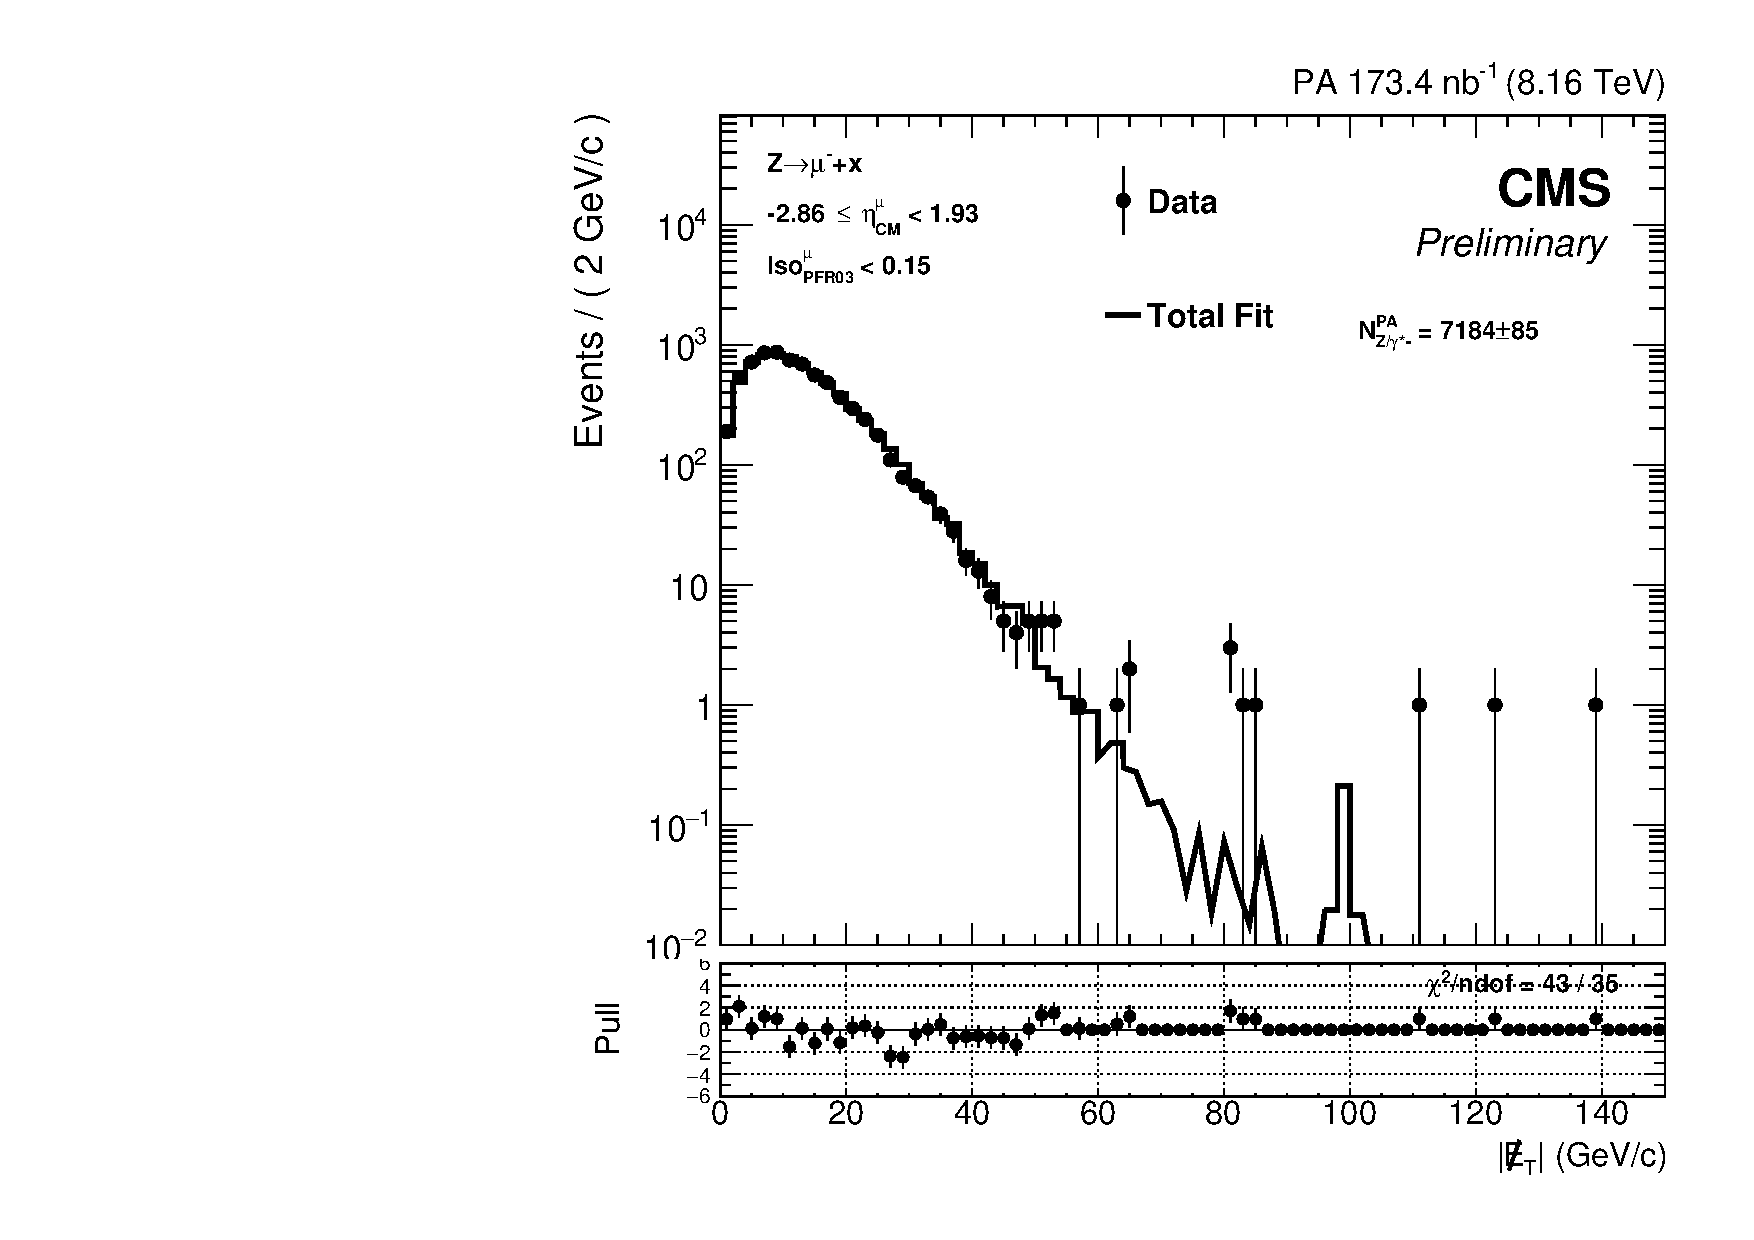
\includegraphics[width=0.4\textwidth]{Figures/WBoson/Analysis/Correction/Recoil/CheckFits/Z/Recoil_ScalingGauss/PLOT_MET_DATA_ZToMuMi_PA_Model_TEMP_DY_MuEtaCM_m286_193_MuIso_0_15.pdf}
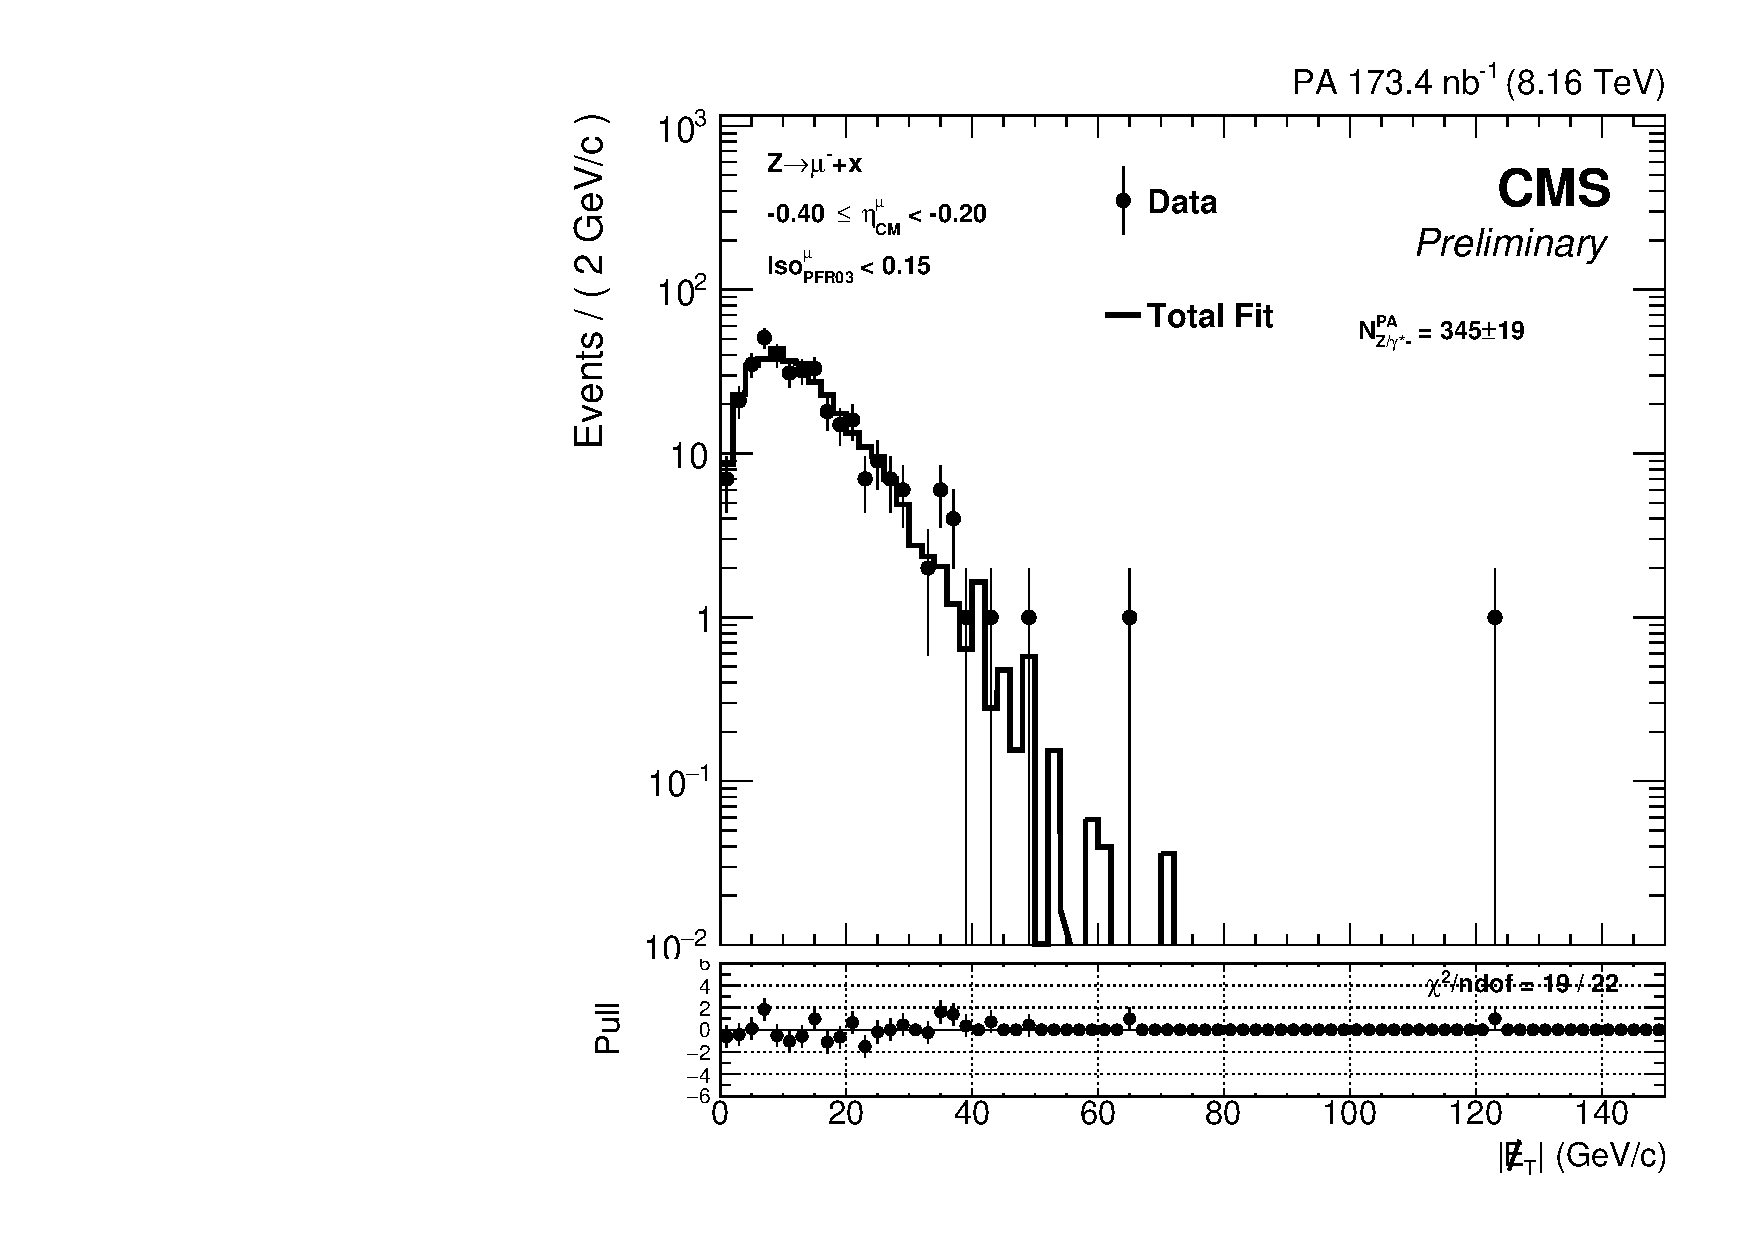
\includegraphics[width=0.4\textwidth]{Figures/WBoson/Analysis/Correction/Recoil/CheckFits/Z/Recoil_ScalingGauss/PLOT_MET_DATA_ZToMuMi_PA_Model_TEMP_DY_MuEtaCM_m40_m20_MuIso_0_15.pdf} 
\caption{A comparison of the MET distribution in data and MC for Z boson selected events.
The left plot corresponds to the full pseudorapidity range in the analysis while the right one corresponds to an specific pseudorapidity bin. The recoil correction using the gaussian scaling method has been applied to MC.}
\label{fig:recoilClosure}
\end{center}
\end{figure}

\clearpage

\subsubsection{Recoil correction in the signal region}\label{sec:WBoson_Analysis_RecoilSignal}

In this section the \W signal in data is extracted following the procedure in \sect{sec:WBoson_Analysis_SignalExtraction}. The recoil corrections are applied to the MC using the 3 methods detailed in \sect{recoilCorr} in order to determine which one works better. \fig{fig:recoilCorrWreg} shows the data fits in the \W region with the scaling method in the general case (top left), gaussian case (top right) and the smearing method (bottom), for the full pseudorapidity region used in the analysis. As we can observe the fit using the scaling method in the gaussian case is the one giving a better fit, so it will be the one used as nominal method in the analysis.
%Also, the difference on the number of the extracted \W between the 3 correction methods is at the permil level, so we consider unnecessary to associate a systematic uncertainty on the correction method, given the size of the other systematic uncertainties of the analysis (see \sect{sec:WBoson_Analysis_Systematics}).

\begin{figure}[!h]
\begin{center}
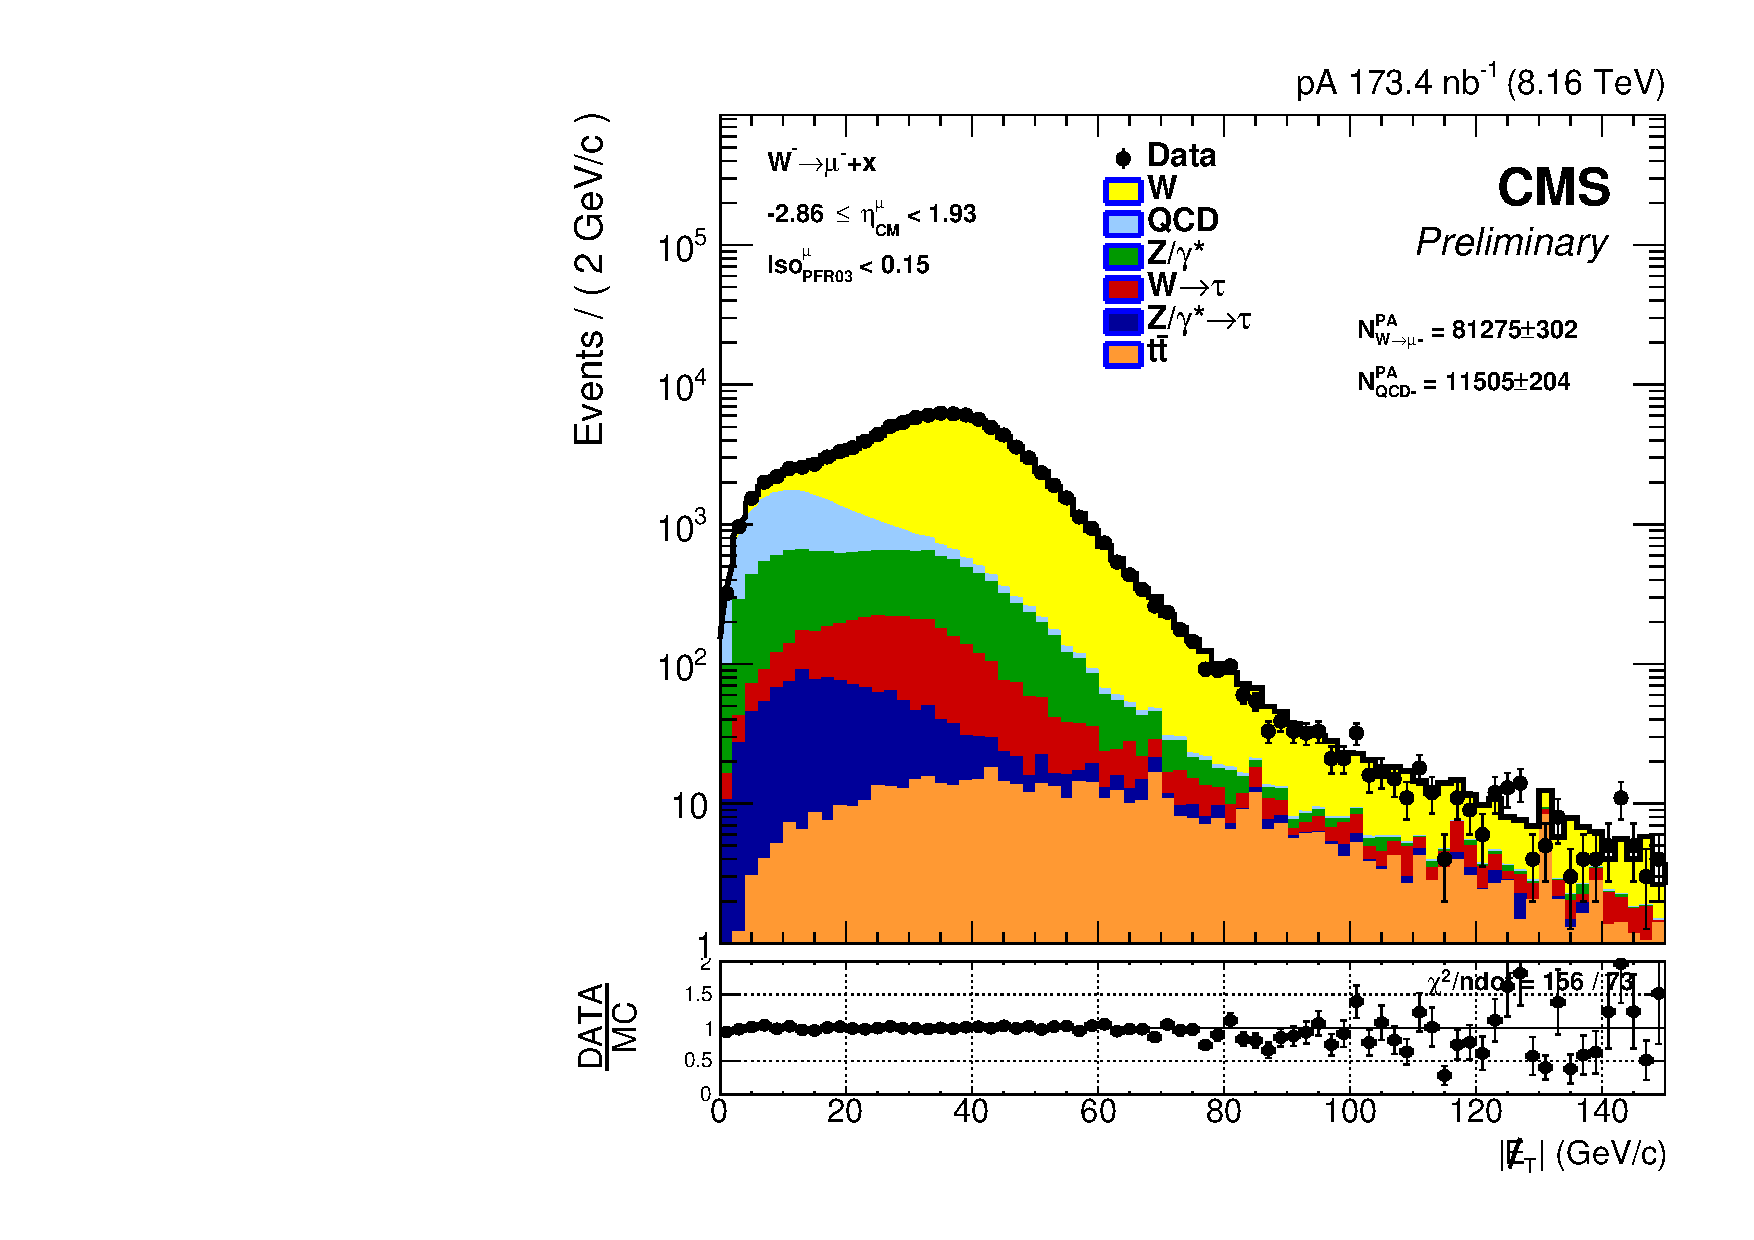
\includegraphics[width=0.4\textwidth]{Figures/WBoson/Analysis/Correction/Recoil/CheckFits/W/Recoil_ScalingGeneral/PLOT_MET_DATA_WToMuMi_PA_Model_TEMP_WDYDYToTauWToTauTTbar_ModifiedRayleigh_QCD_MuEtaCM_m286_193_MuIso_0_15.pdf}
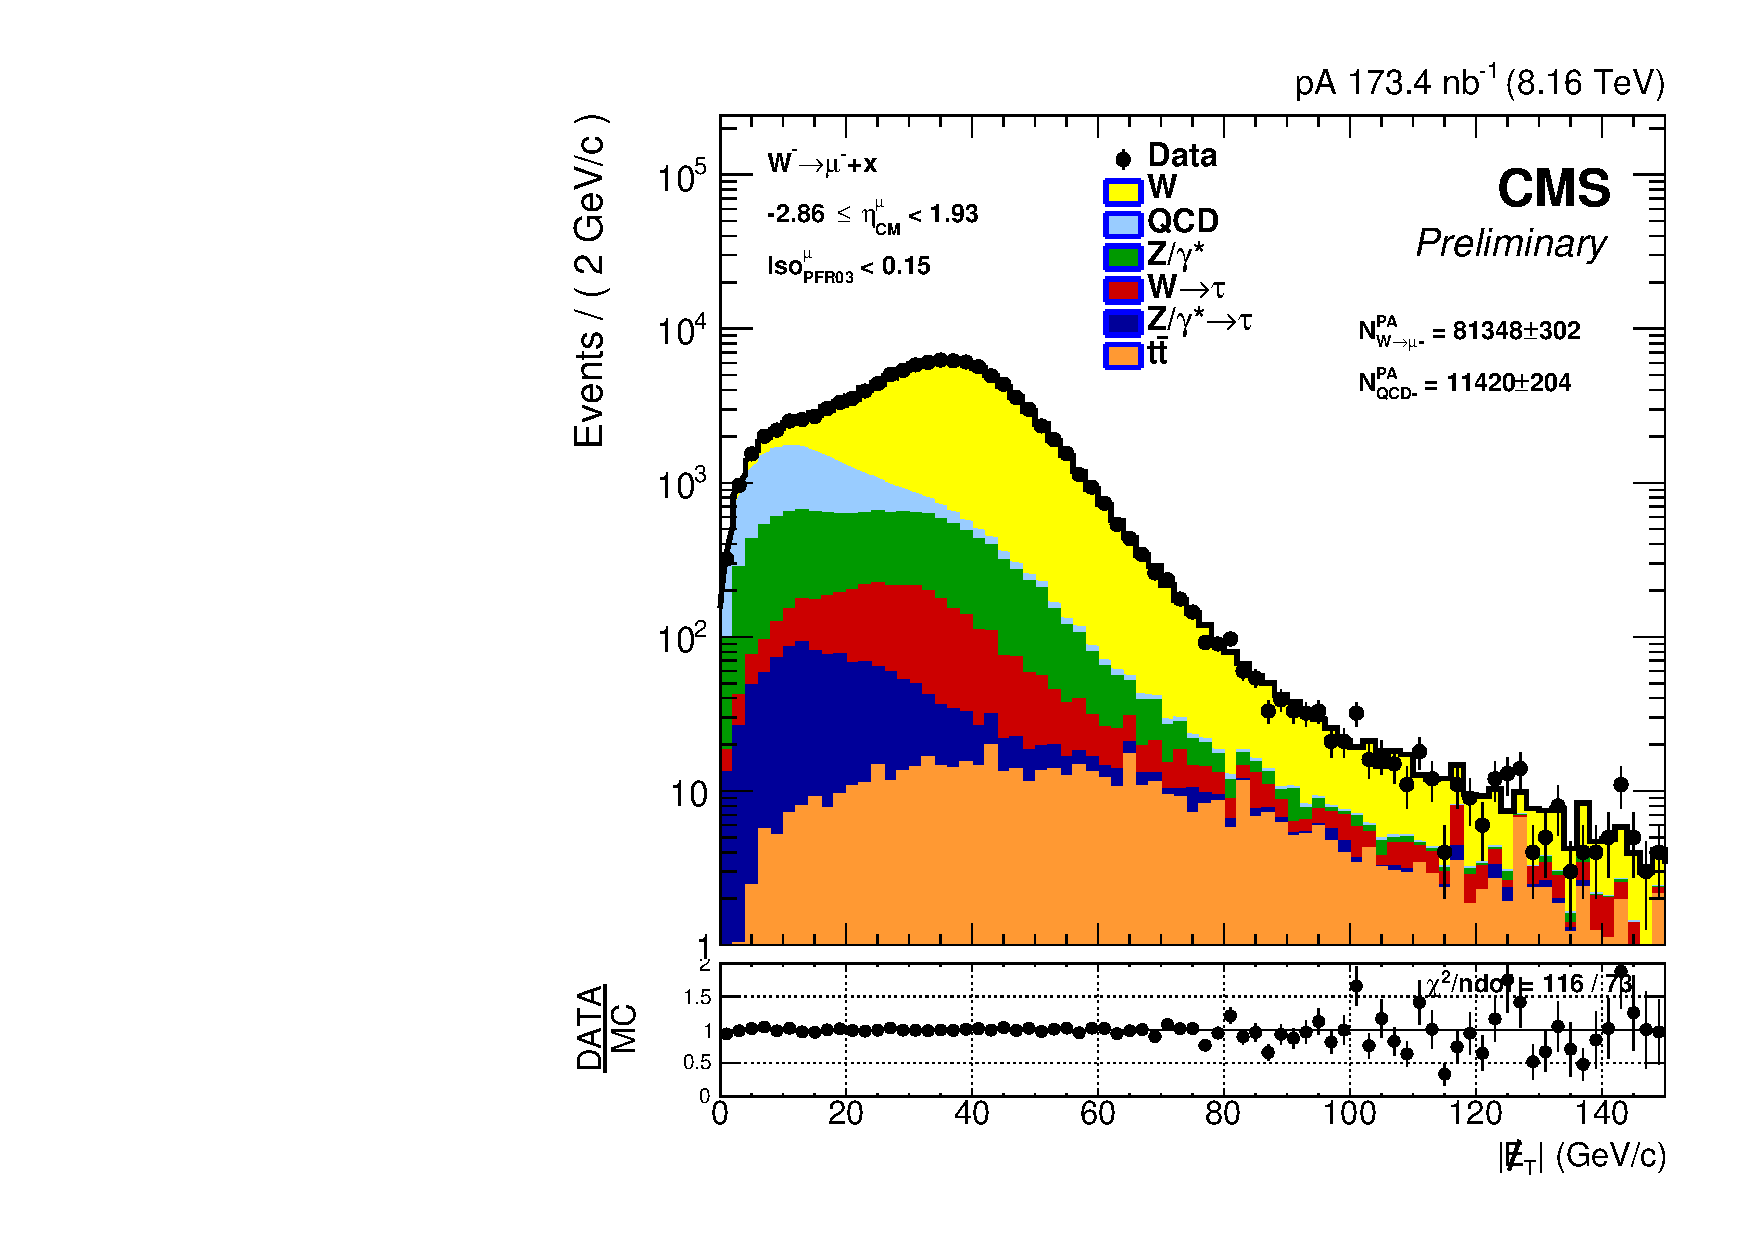
\includegraphics[width=0.4\textwidth]{Figures/WBoson/Analysis/Correction/Recoil/CheckFits/W/Recoil_ScalingGauss/PLOT_MET_DATA_WToMuMi_PA_Model_TEMP_WDYDYToTauWToTauTTbar_ModifiedRayleigh_QCD_MuEtaCM_m286_193_MuIso_0_15.pdf} \\
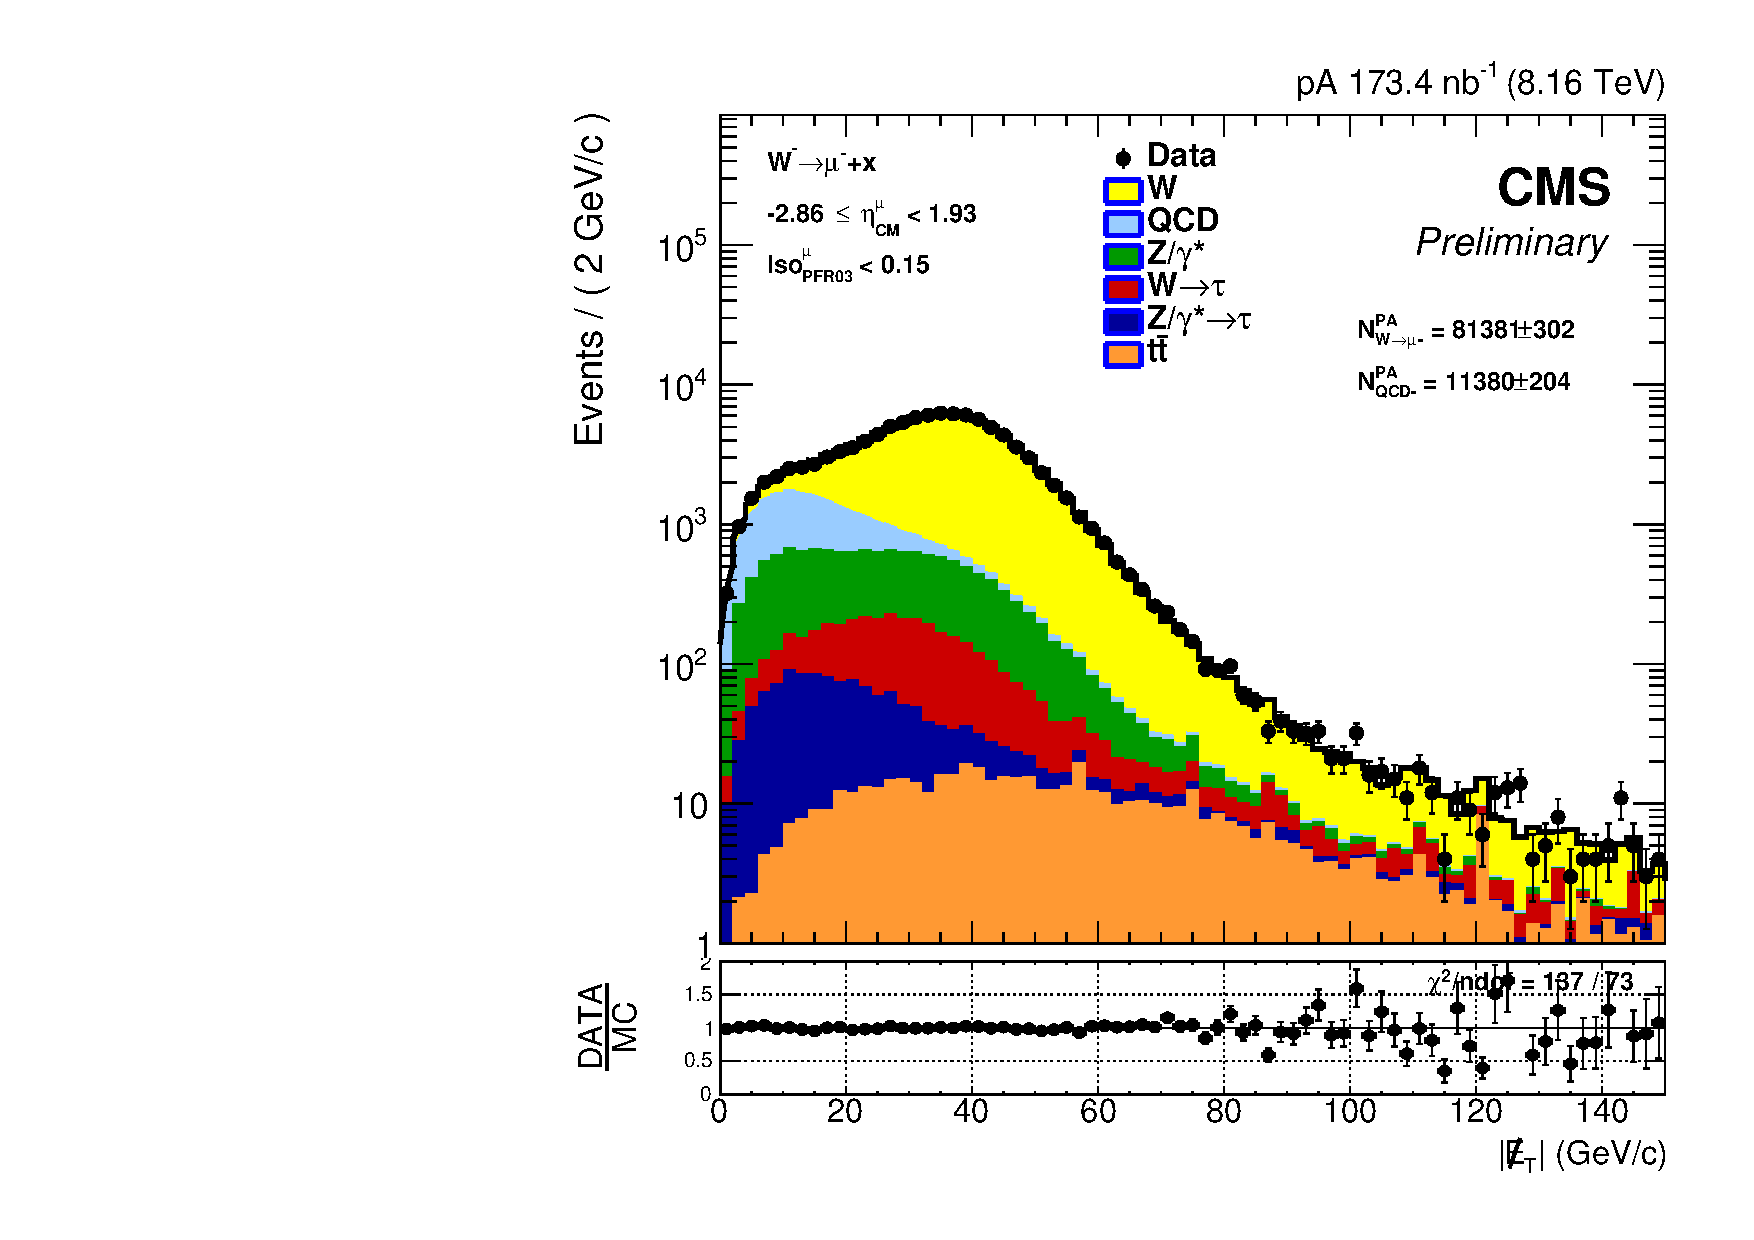
\includegraphics[width=0.4\textwidth]{Figures/WBoson/Analysis/Correction/Recoil/CheckFits/W/Recoil_Smearing/PLOT_MET_DATA_WToMuMi_PA_Model_TEMP_WDYDYToTauWToTauTTbar_ModifiedRayleigh_QCD_MuEtaCM_m286_193_MuIso_0_15.pdf}
\caption{A comparison of the MET distribution in data and MC for W boson selected events in the full pseudorapidity range in the analysis. Different methods to apply the recoil corrections in MC are used in each plot. The top left plot corresponds to the scaling method in the general case, the top right one corresponds to the scaling method in the gaussian case, and the bottom one to the smearing method.}
\label{fig:recoilCorrWreg}
\end{center}
\end{figure}

% END OF SUBSECTION
\clearpage

